\documentclass[a4paper,11pt]{book}


% Package definition
\usepackage[T1]{fontenc}
\usepackage[sfdefault]{atkinson} %% usage de la police Atkinson Hypereligible
\usepackage[scaled=0.85]{beramono} %% pour \texttt
\usepackage{graphicx, subcaption}
\usepackage{setspace}
\usepackage{fancybox}
\usepackage{tikz}
\usepackage{fancyhdr}
\usepackage{pifont}
\usepackage{lipsum} % génère du texte aléatoire
% \usepackage{draftwatermark}
% \SetWatermarkText{CONFIDENTIEL}
% \SetWatermarkColor{gray!20}
% \SetWatermarkFontSize{3cm}
\usepackage[top=2cm, bottom=2.5cm, left=2cm, right=2cm]{geometry} % marge des pages
\usepackage{ragged2e} % justifier texte
\usepackage[french]{babel} 
\usepackage{microtype} %% pour améliorer la typographie, facultatif.

\usepackage{xcolor}
\usepackage{hyperref} %% pour \url avec hyperlien
\usepackage{listings} %% To insert code (Java, Python, etc)
\usepackage[linesnumbered,ruled,vlined]{algorithm2e} %% Pseudo-code

% ----- AJOUT 
\usepackage[htt]{hyphenat}
\usepackage{microtype}
\usepackage{wrapfig}
\usepackage{tabularx}
 \usepackage{amsmath}
%\let\cleardoublepage\clearpage
% -----


%\pagestyle{fancy} % Activer le style fancy
\renewcommand{\headrulewidth}{0pt} % Retrait header
\renewcommand{\familydefault}{\sfdefault}

\newcommand{\titreMemoire}{Analyse empirique et optimisation algorithmique d'un outil de métamodélisation MetaDONE} 

\newcommand{\auteurMemoire}{Carine POCHET}

\newcommand{\diplome}{\textbf\textit{{Décommenter la ligne de redéfinition de la commande \texttt{diplome}}}}
%% MASTER 60
%\renewcommand{\diplome}{Mémoire présenté en vue de l'obtention du grade de Master 60 en Sciences Informatiques}
%% MASTER 120
\renewcommand{\diplome}{Mémoire présenté en vue de l'obtention du grade de Master 120 en Sciences Informatiques}

\newcommand{\anneeacademique}{2025-2026}

\newcommand{\promoteur}{Prof. Vincent ENGLEBERT}
%% laisser vide si pas de co-promoteur
\newcommand{\copromoteur}{} 


%% fichier de configuration et de personnalisation pour vos listings. 
%% Libre à vous de le modifier. 
%% Attention: si vous imprimer en N&B, vérifier que les couleurs restent lisibles et contrastées.


\definecolor{codebg}{rgb}{0.97,0.97,0.97}
\definecolor{javakeyword}{RGB}{0,0,180}
\definecolor{javacomment}{RGB}{0,128,0}
\definecolor{javastring}{RGB}{163,21,21}

\lstdefinelanguage{Java}{
  morekeywords={abstract,assert,boolean,break,byte,case,catch,char,class,const,
    continue,default,do,double,else,enum,extends,final,finally,float,for,goto,
    if,implements,import,instanceof,int,interface,long,native,new,null,package,
    private,protected,public,return,short,static,strictfp,super,switch,
    synchronized,this,throw,throws,transient,try,void,volatile,while},
  sensitive=true,
  morecomment=[l]//,
  morecomment=[s]{/*}{*/},
  morestring=[b]",
}



\lstset{
  language=Java,
  backgroundcolor=\color{codebg},
  basicstyle=\ttfamily\small,
  keywordstyle=\color{javakeyword}\bfseries,
  commentstyle=\color{javacomment}\itshape,
  stringstyle=\color{javastring},
  showstringspaces=false,
  numbers=left,
  numberstyle=\tiny\color{gray},
  numbersep=10pt,
  frame=single,
  tabsize=4,
  captionpos=b,
  breaklines=true,
  breakatwhitespace=true
} %configuration pour les listings

\setlength{\headheight}{13.59999pt}
\setlength{\emergencystretch}{2em} % autorise plus de souplesse pour éviter les débordements de marge


\begin{document}

%%%%%%%%%%%%%%%%%%%%%%%%%%%%%%%%%%%%%%%%%%%%%%%%%%%%%%%%%%%%%%%%%%%%%%%%%%
%% NE PAS EDITER CE FICHIER
%%%%%%%%%%%%%%%%%%%%%%%%%%%%%%%%%%%%%%%%%%%%%%%%%%%%%%%%%%%%%%%%%%%%%%%%%%



\fancyfoot[C]{\thepage} % Retrait footer
    \pagestyle{fancyplain}
    \begin{tikzpicture}[remember picture,overlay]
        \node[anchor=north west,yshift=-30pt,xshift=30pt]
            at (current page.north west)
            {
\includegraphics[height=5cm]{img/FAC_informatique.png}};
    \end{tikzpicture}
    
\centerline{UNIVERSITÉ DE NAMUR}
\centerline{Faculté d'informatique}
\centerline{Année académique \anneeacademique}

\vspace{4cm}

\begin{center}
	\fbox{ \begin{minipage}[c][5.4cm]{9.6cm}
            \large
            \begin{spacing}{1.2}
                \begin{center}
                    \centering \textbf{\titreMemoire}
                    \vspace{1cm}
                    
                    \auteurMemoire
                \end{center}
            \end{spacing}
        \end{minipage}}
\end{center}

    % ==> CADRE A COMPLETER
    \vspace{2.8cm}
    \centerline{
        \begin{minipage}[c][3cm]{9.6cm} 
            \begin{spacing}{2}
                \begin{center}
                    \leftline{........................ (Signature pour approbation du dépôt - REE art. 40)}
                    \leftline{Promoteur : \promoteur}
                    \ifx\copromoteur\empty\leftline{Co-promoteur : \copromoteur}\else\fi
                \end{center}
            \end{spacing}
        \end{minipage}
    }

    \vspace{2cm}
    \centering\mbox{
        \begin{minipage}[c][5cm]{9.6cm}
            \begin{spacing}{2}
                \begin{center}
                    \vspace{6.4cm}
                    \centerline{\large\diplome}
                    %\newline
                    \vspace{1.6cm}
                    \centerline{ Faculté d'Informatique --- Université de Namur}
                   % \newline 
                    \centerline{ RUE GRANDGAGNAGE, 21 $\bullet$ B-5000 NAMUR  $\bullet$ BELGIUM}
                \end{center}
            \end{spacing}
        \end{minipage}
    }

%%%%%%%%%%%%%%%%%%%%%%%%%%%%%%%%%%%%%%%%%%%%%%%%%%%%%%%%%%%%%%%%%%%%%%%%%%%%%%%%%%%%%%%%%
\thispagestyle{empty}

\justifying

\clearpage
\noindent\textbf{\huge Remerciements}

\bigskip

\begin{quote}
Mes premiers remerciements vont au professeur Vincent Englebert, qui m'a proposé ce sujet et m'a accompagnée tout au long de ce travail. Je le remercie pour sa disponibilité constante, son honnêteté et la précision de ses retours qu’il m’a accordés à chaque étape, dans les moments d'avancement comme de doute.

Je tiens également à remercier mes parents pour leur soutien inconditionnel pendant ces années d'études. Une mention particulière à ma mère, qui m'a suivie tout au long de ce mémoire, indépendamment de la technicité du sujet.

Mes remerciements vont enfin à mes camarades et amis, en particulier Romain, dont les discussions et l’entraide ont contribué à faire de ces années une expérience enrichissante autant sur le plan académique qu’humain.
\end{quote}


\clearpage
\noindent\textbf{\huge Résumé}
\bigskip

\begin{quote}
MetaDONE est un outil MetaCASE bâti sur l'architecture MetaL$_2$ et reposant sur une couche de persistance JPA. Ce mémoire étudie empiriquement les performances de MetaDONE afin d'identifier ses goulots d'étranglement et de proposer des optimisations algorithmiques compatibles avec ses principes architecturaux, en particulier le Design by Contract.

Quatre scénarios couvrant la construction de métamodèles, le chargement de scripts GraSyLa, la boucle de dispatch de visualisation et la scalabilité de la création de modèles concrets ont été conçus, instrumentés et mesurés. Pour chaque scénario, l'analyse a suivi un cycle complet : benchmark, identification de la cause racine, conception d'une optimisation, validation expérimentale du gain.

Deux optimisations algorithmiques ont été retenues : la mise en cache de la vérification d'appartenance dans \texttt{ConcreteModel\_impl}, ramenant la construction de métamodèles de $O(N^2)$ à $O(N)$, et la correction d'une asymétrie de conception dans \texttt{\_createRole}, ramenant la création d'arcs de $O(N^2)$ à un plancher proche de $O(N \log N)$, avec un gain médian de $4{,}39\times$ à $N = 5\,000$. Deux autres optimisations ont été rejetées sur la base des mesures : l'une sans effet sur le backend utilisé, l'autre violant le principe Design by Contract. Un profilage live de l'application Eclipse complète l'analyse en quantifiant le coût réel du pipeline de visualisation.

Ce travail montre qu'un gain substantiel de performance est compatible avec le respect des principes architecturaux de l'outil, à condition d'exploiter les invariants du système plutôt que de les contourner.
\end{quote}
\bigskip
\noindent\textbf{Mots-clés} : MetaDONE, MetaCASE, méta-modélisation, optimisation de performance, complexité algorithmique, Design by Contract, profilage, JPA, benchmark

\vspace{0.75cm}

\noindent\textbf{\huge Abstract}
\bigskip

\begin{quote}
MetaDONE is a MetaCASE tool built on the MetaL$_2$ architecture and relying on a JPA persistence layer. This dissertation empirically investigates the performance of MetaDONE in order to identify its bottlenecks and to propose algorithmic optimisations compatible with its architectural principles, in particular Design by Contract.

Four scenarios covering metamodel construction, GraSyLa script loading, the visualisation dispatch loop and the scalability of concrete model creation were designed, instrumented and measured. Each scenario followed a complete cycle: benchmark, root-cause identification, optimisation design, experimental validation of the gain.

Two algorithmic optimisations were retained: caching the definition-membership check in \texttt{ConcreteModel\_impl}, reducing metamodel construction from $O(N^2)$ to $O(N)$, and correcting a design asymmetry in \texttt{\_createRole}, reducing role creation from $O(N^2)$ to a floor close to $O(N \log N)$, with a median gain of $4{.}39\times$ at $N = 5\,000$. Two further candidates were rejected on the basis of measurements: one had no effect on the chosen backend, the other violated the Design by Contract principle. A live profiling session of the Eclipse application complements the analysis by quantifying the actual cost of the visualisation pipeline.

This work demonstrates that substantial performance gains are compatible with the architectural principles of the tool, provided that system invariants are exploited rather than circumvented.
\end{quote}
\bigskip
\noindent\textbf{Keywords} : MetaDONE, MetaCASE, metamodelling, performance optimisation, algorithmic complexity, Design by Contract, profiling, JPA, benchmark


\tableofcontents

\clearpage
\section*{Acronymes}

\begin{description}
    \item[ANTLR:]  ANother Tool for Language Recognition
    \item[API:]    Application Programming Interface
    \item[AST:]    Abstract Syntax Tree
    \item[ATL:]    ATLAS Transformation Language
    \item[BPMN:]   Business Process Model and Notation
    \item[CASE:]   Computer-Aided Software Engineering
    \item[CPU:]    Central Processing Unit
    \item[CV:]     Coefficient of Variation
    \item[DbC:]    Design by Contract
    \item[DSL:]    Domain Specific Language
    \item[DSM:]    Domain Specific Modeling
    \item[DSML:]   Domain Specific Modeling Language
    \item[EMF:]    Eclipse Modeling Framework
    \item[GC:]     Garbage Collector
    \item[GoF:]    Gang of Four
    \item[GOPPRR:] Graph, Object, Property, Port, Role, Relationship
    \item[GPL:]    General Purpose Modeling Language
    \item[GraSyLa:] Graphical Symbolic Language
    \item[GUI:]    Graphical User Interface
    \item[I/O:]    Input/Output
    \item[JDBC:]   Java Database Connectivity
    \item[JDK:]    Java Development Kit
    \item[JDO:]    Java Data Objects
    \item[JFR:]    Java Flight Recorder
    \item[JIT:]    Just-In-Time (compilation)
    \item[JMC:]    Java Mission Control
    \item[JPA:]    Java Persistence API
    \item[JVM:]    Java Virtual Machine
    \item[KM3:]    Kernel MetaMetaModel
    \item[LHS:]    Left-Hand Side
    \item[MDA:]    Model-Driven Architecture
    \item[MDE:]    Model-Driven Engineering
    \item[MML:]    Metamodeling Language
    \item[MOF:]    Meta Object Facility
    \item[OID:]    Object Identifier
    \item[OMG:]    Object Management Group
    \item[ORM:]    Object-Relational Mapping
    \item[OSGi:]   Open Services Gateway initiative
    \item[OWL:]    Web Ontology Language
    \item[PID:]    Process Identifier
    \item[RCP:]    Rich Client Platform
    \item[RDF:]    Resource Description Framework
    \item[REST:]   Representational State Transfer
    \item[RHS:]    Right-Hand Side
    \item[SQL:]    Structured Query Language
    \item[SSD:]    Solid State Drive
    \item[SVG:]    Scalable Vector Graphics
    \item[SVN:]    Subversion
    \item[SWT:]    Standard Widget Toolkit
    \item[TDP:]    Thermal Design Power
    \item[UI:]     User Interface
    \item[UML:]    Unified Modeling Language
    \item[XMI:]    XML Metadata Interchange
    \item[XML:]    eXtensible Markup Language
    \item[ZGC:]    Z Garbage Collector
\end{description}


\renewcommand{\headrulewidth}{1pt} % Retrait header

\pagestyle{fancy}

\chapter{Introduction}
\label{chap:introduction}

Concevoir et maintenir des systèmes logiciels de grande taille suppose de pouvoir naviguer dans une multiplicité de représentations --- code, diagrammes, documents --- sans perdre la cohérence entre elles. Les approches traditionnelles, centrées sur l'écriture manuelle du code, peinent à tenir ce contrat à mesure que la complexité s'accroît~: les artefacts dérivent, les contraintes métier se diluent dans l'implémentation et la documentation prend du retard.

C'est dans ce contexte que s'inscrit l'Ingénierie Dirigée par les Modèles (\textit{Model-Driven Engineering}, MDE). Cette méthodologie place le modèle — une représentation abstraite et simplifiée du système — au cœur du processus de développement. En se concentrant sur les concepts métier essentiels et en faisant abstraction des détails d'implémentation, le MDE permet, par le biais de transformations automatisées, de générer des artefacts tels que du code source ou de la documentation technique.

Pour soutenir cette approche, des outils de génie logiciel assisté par ordinateur, appelés outils CASE (\textit{Computer-Aided Software Engineering}), ont été développés. Ces outils souffrent cependant d'une rigidité méthodologique : ils sont limités à un ensemble fixe de notations de modélisation, codées en dur par le fournisseur. Pour pallier ce manque de flexibilité, les outils MetaCASE, tels que MetaDONE, ont émergé. Ils permettent de définir des langages de modélisation spécifiques à un domaine (\textit{Domain Specific Modeling Languages}, DSML) afin de générer dynamiquement des environnements de modélisation sur mesure.

Si ces outils offrent des gains substantiels en termes de réutilisation et de standardisation, ils font face à un obstacle technique majeur : la scalabilité. Lorsque la taille des modèles augmente, les performances des outils MDE peuvent se dégrader significativement, en particulier lors des phases de persistance et de chargement en mémoire~\cite{kolovos2013research}.

Ce mémoire se concentre sur l'analyse empirique et l'optimisation des performances de MetaDONE, un outil MetaCASE développé à l'Université de Namur~\cite{Eng2007}. MetaDONE repose sur le langage de métamodélisation MetaL, organisé en deux couches complémentaires : MetaL$_1$, le noyau formel qui définit les concepts atomiques de persistance, et MetaL$_2$, la couche d'abstraction qui permet de construire et de manipuler des métamodèles spécifiques à un domaine. À ces deux couches s'ajoute GraSyLa, un DSML déclaratif permettant de spécifier les notations concrètes (graphiques ou textuelles) associées à un métamodèle, dont l'évaluation conditionne directement la réactivité de l'interface utilisateur. La propriété fondamentale qui distingue MetaL de ses concurrents — et qui en fait à la fois la force et la source de défis techniques — est sa réflexivité totale : le langage se décrit lui-même avec ses propres construits, formant un graphe de données dense et cyclique plutôt qu'une arborescence. Cette propriété est indispensable au \textit{bootstrapping} de l'outil, qui peut ainsi s'étendre sans modification du code source, mais elle engendre des surcoûts spécifiques lors de la persistance et du chargement des modèles.

MetaDONE est développé en Java et s'appuie sur l'architecture modulaire OSGi (\textit{Open Services Gateway initiative}), qui permet d'étendre l'outil par des plugins indépendants — support de nouvelles notations (BPMN, réseaux de Petri, diagrammes entité-association), nouveaux mécanismes de persistance — sans modifier le noyau de l'application. Cette extensibilité constitue une contrainte autant qu'un avantage : toute optimisation du noyau doit rester compatible avec l'ensemble des plugins existants, ce qui renforce la nécessité d'une méthodologie de profilage rigoureuse et d'optimisations locales et non invasives.

La question centrale de ce mémoire est la suivante : dans quelle mesure les surcoûts liés à la réflexivité et à la persistance de MetaDONE sont-ils mesurables et réductibles, sans remettre en cause les garanties architecturales de l'outil ?

Pour y répondre, nous adoptons une démarche empirique structurée autour de scénarios représentatifs des usages réels de MetaDONE, en appliquant un cycle itératif mesure--analyse--optimisation. Les outils de profilage Java retenus --- Java Flight Recorder pour les mesures globales à faible surcoût, et async-profiler pour l'analyse fine des méthodes chaudes par flamegraphs --- permettent de localiser avec précision les goulots d'étranglement sans biais d'observation significatif.

Les principales contributions de ce travail sont les suivantes. Premièrement, l'identification empirique de quatre goulots d'étranglement caractéristiques de MetaDONE, situés respectivement dans la construction de métamodèles, le chargement de scripts GraSyLa, la boucle de visualisation et la création de modèles concrets à grande échelle. Deuxièmement, l'implémentation et la validation expérimentale de deux optimisations algorithmiques compatibles avec le Design by Contract de l'outil~: la mise en cache de la vérification d'appartenance dans \texttt{ConcreteModel\_impl} (ramenant la construction de métamodèles de $O(N^2)$ à $O(N)$) et la correction d'une asymétrie de conception dans \texttt{\_createRole} (ramenant la création de rôles de $O(N^2)$ à un plancher proche de $O(N \log N)$, soit un gain médian de $4{,}39\times$ mesuré à $N = 5\,000$ sur 10 répétitions par campagne). Troisièmement, le rejet motivé de deux candidates d'optimisation~: l'une dont les mesures montrent qu'elle n'a aucun effet sur le backend utilisé, l'autre dont l'implémentation violerait le principe Design by Contract de l'outil. Enfin, un profilage live de l'application Eclipse qui quantifie le coût réel du pipeline de visualisation et oriente les perspectives d'amélioration.

Ce mémoire s'organise comme suit. Le chapitre~\ref{chap:etat_art} établit l'état de l'art du MDE, des outils MetaCASE et des problématiques de scalabilité et de persistance de modèles. Le chapitre~\ref{chap:architecture} présente l'architecture interne de MetaDONE dans laquelle s'inscrivent les optimisations. Le chapitre~\ref{chap:methodologie} décrit la méthodologie expérimentale adoptée. Le chapitre~\ref{chap:developpement} constitue le cœur du travail : il présente, pour chaque scénario, le diagnostic des goulots d'étranglement, les optimisations implémentées et leur évaluation quantitative. Le chapitre~\ref{chap:discussion} discute les résultats en les replaçant dans le contexte architectural de MetaDONE et identifie les perspectives d'amélioration. Le chapitre~\ref{chap:conclusion} conclut le mémoire.
\chapter{État de l'art}
\label{chap:etat_art}

% ---------------------------------------------------------------
% ---------------------------------------------------------------
\section{Model-Driven Engineering}
\label{sec:mde}
% ---------------------------------------------------------------
% ---------------------------------------------------------------

L'émergence de l'Ingénierie Dirigée par les Modèles (MDE) répond à la nécessité de simplifier le développement de systèmes logiciels complexes et d'automatiser leurs cycles de production. En plaçant les modèles au centre du processus d'ingénierie, cette approche facilite le partage d'une vision et de connaissances communes entre les parties prenantes techniques et non techniques~\cite{da2015model}. L'évolution vers la MDE permet également de s'abstraire des complexités liées aux environnements informatiques sous-jacents en privilégiant des langages et des plateformes de plus haut niveau~\cite{schmidt2006model}. Cette élévation du niveau d'abstraction repose sur une séparation rigoureuse des préoccupations : les architectes peuvent ainsi se concentrer sur les décisions métier essentielles, indépendamment des spécificités et des fluctuations des technologies cibles~\cite{brown2004model}.

Pour représenter fidèlement des systèmes d'envergure, une approche multi-modèles est généralement indispensable~\cite{brown2004model,da2015model}. Chaque modèle offre une vue partielle et simplifiée, se focalisant sur des perspectives spécifiques (structurelle, comportementale ou physique) afin de maîtriser la complexité croissante des solutions d'entreprise.

La MDE englobe diverses méthodologies telles que l'Architecture Dirigée par le Modèle (MDA), les Software Factories ou l'ingénierie des Domain Specific Languages (DSL). Bien que ces approches diffèrent dans leurs objectifs et leurs outils, elles s'appuient sur des techniques avancées telles que la méta-modélisation, la transformation de modèles et la génération de code pour automatiser la création ou l'exécution de systèmes~\cite{da2015model}.

% ---------------------------------------------------------------
\subsection{CASE et MetaCASE}
\label{sec:case-metacase}
% ---------------------------------------------------------------

Les premiers outils utilisés pour automatiser les tâches de conception et de documentation sont les outils CASE (Computer-Aided Software Engineering). Ces outils supportent généralement un nombre fixe de méthodologies (comme UML ou les diagrammes de flux de données) qui sont codées en dur par le fournisseur. Dans un outil CASE standard, l'architecture est à deux niveaux : les conceptions système sont stockées dans un référentiel dont le schéma est figé~\cite{isazadeh1997case}. Cette rigidité est l'un des principaux freins à l'adoption de méthodologies innovantes ou spécifiques à un domaine, car seul le vendeur peut modifier le fonctionnement de l'outil.

Les technologies MetaCASE approchent l'automatisation de manière dynamique. Elles permettent de générer dynamiquement des environnements de modélisation adaptés à n'importe quelle méthode ou domaine. Les MetaCASE reposent sur une architecture à trois niveaux (voir figure \ref{isa-fig}) où le métamodèle de la méthode n'est pas programmé dans le code source de l'outil, mais stocké comme une donnée modifiable dans le référentiel~\cite{isazadeh1997case}.
\begin{itemize}
    \item Niveau Meta : les développeurs construisent les composants génériques et définissent le méta-modèle.
    \item Niveau Environnement : le méta-modèle est utilisé pour bâtir un outil CASE spécifique à l'organisation.
    \item Niveau Utilisateur : les développeurs utilisent cet outil sur mesure pour créer les produits logiciels.
\end{itemize}
\begin{figure}[h]
\centering
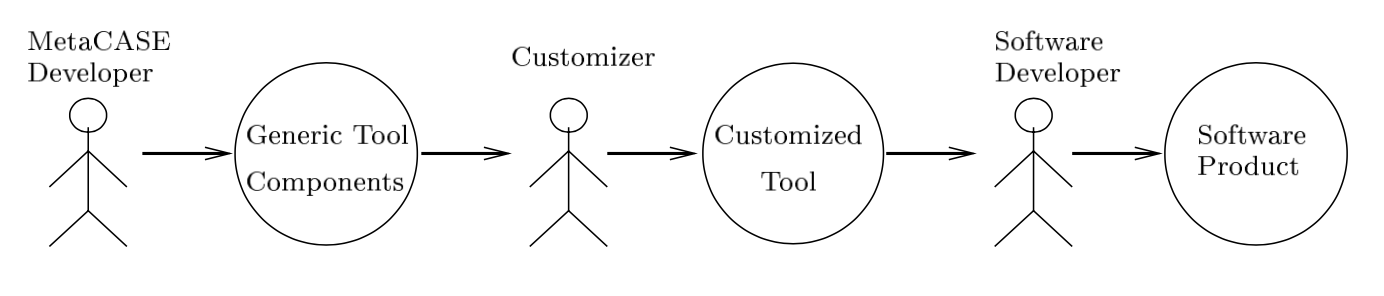
\includegraphics[width=0.8\textwidth]{img/etat_art/metacase3level.png}
\caption{Vue d'ensemble des 3 niveaux d'architecture MetaCASE~\cite{isazadeh1997case}}
\label{isa-fig}
\end{figure}
MetaDONE s'inscrit pleinement dans cette architecture à trois niveaux, en proposant un framework méta générique, un mécanisme de définition d'environnements CASE par méta-modélisation et un niveau utilisateur pour la création de modèles concrets.

% ---------------------------------------------------------------
% ---------------------------------------------------------------
\section{Langages de modélisation}
\label{sec:langages}
% ---------------------------------------------------------------
% ---------------------------------------------------------------

La MDE repose sur l'utilisation de langages de modélisation pour exprimer les différentes facettes d'un système. Ces langages se distinguent par leur niveau de généralité~: certains visent une applicabilité universelle tandis que d'autres ciblent un domaine précis. Comprendre cette distinction est essentiel pour saisir pourquoi des outils comme MetaDONE ont été conçus, et quelles contraintes techniques leur usage impose.

% ---------------------------------------------------------------
\subsection{Langages généraux de modélisation}
\label{sec:langages-generaux}
% ---------------------------------------------------------------

Les premiers langages à s'imposer dans le contexte MDE sont des langages à usage général (\textit{General Purpose Modeling Languages}, GPL), dont le représentant le plus emblématique est UML (\textit{Unified Modeling Language}). Adopté comme standard par l'OMG\footnote{Object Management Group, \url{https://www.omg.org}}, UML a été conçu pour unifier les nombreuses pratiques de modélisation alors en vigueur dans l'industrie~\cite{france2007mde}. 
\begin{wrapfigure}{r}{5.5cm}
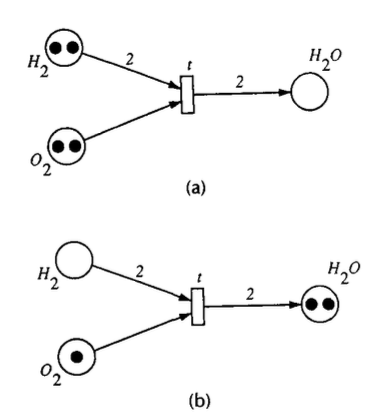
\includegraphics[width=5.5cm]{img/etat_art/petri.png}
\caption{Exemple d'illustration de la réaction chimique $2H_2 + 0_2 \rightarrow 2H_20$ avec les réseaux de Petri~\cite{murata1989petri}}
\label{murata-fig}
\end{wrapfigure} 
Sa force réside dans sa polyvalence~: il couvre les aspects structurels (diagrammes de classes, de composants), comportementaux (machines à états, diagrammes de séquence) et de déploiement d'un système logiciel.

Cependant, cette généralité devient rapidement un frein. En cherchant à tout couvrir, UML est devenu extrêmement large et complexe. De plus, il ne permet pas de définir entièrement les relations entre ses propres diagrammes, et la spécification de comportements détaillés y reste difficile~\cite{koshima2016distributed}. Le mécanisme d'extension officiel d'UML, les \textit{profils}, est largement reconnu comme insuffisant~: il ne permet que d'adapter superficiellement la syntaxe du langage, sans modifier le métamodèle ni la sémantique sous-jacente~\cite{Eng2007}.


À côté d'UML, les \textbf{réseaux de Petri} constituent un autre langage de modélisation à usage général, orienté cette fois vers la spécification formelle de systèmes concurrents et distribués~\cite{reisig1985petri,murata1989petri}. Un réseau de Petri est défini par un ensemble de \textit{places} (états potentiels du système), de \textit{transitions} (événements pouvant survenir) et d'\textit{arcs orientés} les reliant. Des \textit{jetons} circulent dans le réseau pour représenter l'état courant du système (voir exemple figure \ref{murata-fig}). Leur sémantique formelle bien établie les rend particulièrement adaptés à l'analyse de propriétés telles que la vivacité, la sûreté ou l'absence d'interblocage. Ils servent d'ailleurs d'exemple canonique dans la documentation de MetaDONE pour illustrer la définition d'un métamodèle avec MetaL$_2$~\cite{techreportgrasylaversion2}.

Si ces deux langages partagent l'ambition d'être universellement applicables, ils souffrent d'une limite commune~: en voulant s'adapter à tous les domaines, ils n'en servent aucun de manière optimale. Un expert métier confronté à un diagramme de classes UML ou à un réseau de Petri doit d'abord maîtriser le formalisme avant de pouvoir exprimer ses connaissances. C'est précisément cette friction qui a motivé l'émergence des langages spécifiques au domaine.

% ---------------------------------------------------------------
\subsection{Domain Specific Languages et DSML}
\label{sec:dsl-dsml}
% ---------------------------------------------------------------

Face aux limites des GPL, une approche complémentaire s'est imposée~: la conception de \textit{Domain Specific Languages} (DSL), c'est-à-dire des langages de modélisation conçus pour un domaine applicatif précis plutôt que pour une utilisation générale~\cite{schmidt2006model}. Lorsqu'un tel langage est doté d'un métamodèle explicite constituant sa syntaxe abstraite, d'une notation concrète (textuelle ou graphique) et d'une sémantique formalisée, on parle de \textit{Domain Specific Modeling Language} (DSML)~\cite{koshima2016distributed}.

La distinction fondamentale entre un modèle et son langage repose sur la séparation entre \textbf{syntaxe abstraite} et \textbf{syntaxe concrète}. La syntaxe abstraite décrit les concepts du langage et leurs relations~; elle est spécifiée par un métamodèle. La syntaxe concrète est la surface visible par l'utilisateur~: la notation graphique, textuelle ou mixte avec laquelle il interagit~\cite{koshima2016distributed}. Dans MetaDONE, GraSyLa (\textit{Graphical Symbolic Language}) joue précisément ce rôle de pont entre syntaxe abstraite et syntaxe concrète~: c'est un DSML dédié à la définition des notations concrètes à partir des métamodèles MetaL$_2$~\cite{techreportgrasylaversion2}.

L'intérêt principal d'un DSML est de permettre aux experts du domaine de travailler directement avec leurs propres concepts, sans devoir maîtriser une technologie de modélisation générique~\cite{koshima2016distributed}. En conséquence, la qualité des produits logiciels s'améliore, les coûts de conception et de développement diminuent, et la longévité des systèmes augmente~\cite{koshima2016distributed}. Des études empiriques suggèrent que l'adoption de DSML peut améliorer la productivité d'un facteur cinq à dix par rapport aux approches par langage général~\cite{kelly2008dsm}.


\begin{wrapfigure}{l}{3.8cm}
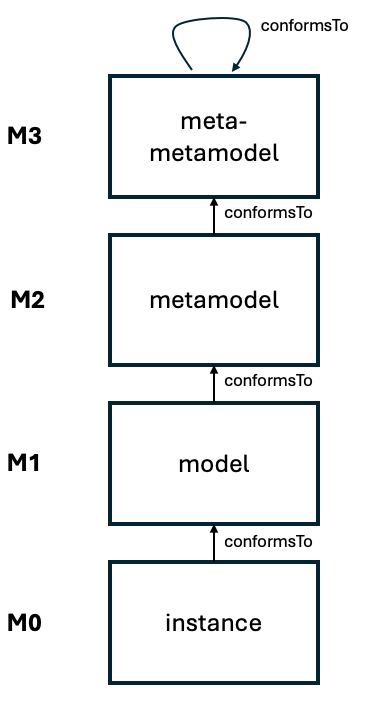
\includegraphics[width=3.5cm]{img/etat_art/omg4level.png}
\caption{Représentation des 4 niveaux d'abstraction de l'OMG}
\label{fig:omf4level}
\end{wrapfigure} 
Du point de vue de l'architecture MDE, un DSML est lui-même un modèle~: il est conforme à un \textit{métamodèle} (qui en définit la structure), lequel est conforme à un \textit{métamétamodèle} (qui définit le langage de métamodélisation lui-même). Cette hiérarchie à trois niveaux --- model, meta-model, meta-meta-model --- est représentée dans l'architecture à quatre couches de l'OMG (M0 à M3), dont MOF (\textit{Meta Object Facility}) constitue le niveau supérieur~\cite{da2015model} (voir figure~\ref{fig:omf4level}). MetaDONE adopte une approche analogue, supportant les niveaux M1, M2 et M3 de la hiérarchie OMG au sein d'un même environnement réflexif~\cite{Eng2007}.


Il convient de noter que les outils MetaCASE et les environnements DSM (\textit{Domain-Specific Modeling}) modernes reposent sur des \textit{Metamodeling Languages} (MML) — comme MOF, Kermeta, KM3 ou GOPPRR — pour définir leurs DSL. Ces langages présentent cependant plusieurs limitations communes~: l'incapacité ou la difficulté à établir des liens entre des construits sémantiquement liés répartis dans des (méta)modèles distincts~; la restriction des niveaux de modélisation éditables, généralement limités à M2 (méta-modèle) et M1 (modèle); l'impossibilité pour les relations de traverser les frontières entre niveaux d'abstraction, connue sous le nom de \textit{strict metamodelling}; et le codage en dur de diverses informations — le MML lui-même, des éléments de syntaxe concrète, l'interface graphique ou les mécanismes de versionnement~\cite{Eng2007}.

% ---------------------------------------------------------------
\section{Tour d'horizon des outils MetaCASE}
\label{sec:metacase-outils}
% ---------------------------------------------------------------

La prolifération des DSML dans l'industrie a conduit au développement d'outils MetaCASE capables de les générer dynamiquement à partir de métamodèles. Bien que ces outils partagent l'architecture à trois niveaux décrite à la section~\ref{sec:case-metacase}, leurs choix de conception les différencient significativement~\cite{Eng2007}. Nous retenons ci-dessous trois outils représentatifs des principales familles d'approches~: MetaEdit+ pour sa maturité industrielle, WebGME pour sa dimension collaborative web, et ConceptBase pour son langage à axiomes flexibles~; chacun éclaire, par contraste, les choix de conception de MetaDONE.

\textbf{MetaEdit+}~\cite{kelly1996metaedit+} est l'un des outils MetaCASE les plus matures industriellement. Il repose sur le langage de métamodélisation GOPPRR (\textit{Graph, Object, Property, Port, Role, Relationship}) et permet le partage de propriétés entre métamodèles. Il offre un support solide pour la modélisation collaborative via un mécanisme de verrouillage fin (\textit{Smart Locks}), mais sa flexibilité reste contrainte~: il n'autorise pas les relations entre niveaux d'abstraction distincts (\textit{strict metamodelling}) et limite le nombre de niveaux M à deux ou trois.

\textbf{WebGME} (\textit{Web-based Generic Modeling Environment})~\cite{webgme} est l'évolution web de GME~\cite{ledeczi2001generic}, un environnement MetaCASE historiquement utilisé dans les domaines de l'embarqué et du génie système. Là où GME reposait sur une application de bureau monoposte, WebGME est une plateforme collaborative hébergée dans le navigateur, offrant l'édition simultanée par plusieurs utilisateurs, un système de versionnement par branches similaire à celui du code source, et une API JavaScript/REST permettant l'intégration avec des outils externes. La définition de DSMLs repose sur un métamodèle de style UML que l'outil interprète pour se configurer automatiquement, et un mécanisme d'héritage prototypique propage les modifications d'un prototype à ses instances. WebGME conserve toutefois la limitation à trois niveaux M et le \textit{strict metamodelling} hérités de GME.

\textbf{ConceptBase}~\cite{jeusfeld2005meta} adopte une approche différente en s'appuyant sur Telos, un langage de métamodélisation très flexible autorisant un nombre de niveaux illimité et un \textit{non-strict metamodelling} (les relations peuvent traverser les niveaux d'abstraction). Sa principale force est un langage déclaratif puissant pour exprimer des contraintes, des règles et des requêtes. Cependant, ses capacités graphiques sont limitées comparées à GraSyLa, et ses axiomes plus rigides que ceux de MetaL~\cite{Eng2007}.

\textbf{MetaDONE}~\cite{Eng2007} se distingue par sa philosophie entièrement \textit{model-driven}~: chaque aspect de l'outil est lui-même un modèle conforme à un métamodèle. Cette propriété, combinée à la \textit{réflexivité universelle} de MetaL, autorise un bootstrapping progressif des fonctionnalités~: l'interface graphique, les notations concrètes, et le contrôle de version peuvent tous être définis ou étendus sans modifier le code source de l'outil. MetaDONE dépasse la limitation des trois niveaux M et permet aux relations de traverser les niveaux d'abstraction (\textit{non-strict metamodelling}). Son dépôt est technologiquement indépendant~: il peut fonctionner avec JDO, RDF ou XMI comme backend de persistance~\cite{Eng2007}. En contrepartie, cette flexibilité engendre une multiplication des couches d'indirection dont le coût en performances doit être évalué et maîtrisé~\cite{Eng2007} --- ce qui constitue l'objet de ce mémoire.

Le tableau~\ref{tab:metacase} synthétise les principales différences de ces MetaCASE.

\begin{table}[h]
\centering
\caption{Comparaison des principaux outils MetaCASE}
\label{tab:metacase}
\small
\begin{tabular}{lllll}
\hline
\textbf{Outil} & \textbf{MML} & \textbf{Niveaux M} &
\textbf{Non-strict} & \textbf{Réflexivité} \\
\hline
MetaEdit+   & GOPPRR    & 2--3      & Non & Non \\
WebGME      & UML-like  & 3         & Non & Non \\
ConceptBase & Telos     & Illimités & Oui & Partielle \\
MetaDONE    & MetaL     & Illimités & Oui & Totale \\
\hline
\end{tabular}
\end{table}

La réflexivité totale de MetaL, qui fait la force de MetaDONE, a une conséquence structurelle directe~: elle augmente la densité du graphe de données stockées dans le dépôt ainsi que la complexité computationnelle des algorithmes de parcours et de gestion. Cette propriété, bénéfique pour l'expressivité du langage, introduit des contraintes spécifiques dès lors qu'il s'agit de sérialiser ou de charger ces données en mémoire. La section suivante examine en détail la nature de ces graphes et leurs implications pour la persistance.

% ---------------------------------------------------------------
% ---------------------------------------------------------------
\section{Les modèles comme graphes}
\label{sec:graphes}
% ---------------------------------------------------------------
% ---------------------------------------------------------------

Les sections précédentes ont présenté la MDE et ses langages de modélisation de manière conceptuelle. Pour comprendre les enjeux de performance propres à MetaDONE, il est nécessaire de descendre au niveau de la représentation concrète des données~: tout modèle MDE est fondamentalement une structure de graphe, et les propriétés particulières du graphe de MetaL engendrent des contraintes techniques spécifiques sur la persistance et le chargement en mémoire.

% ---------------------------------------------------------------
\subsection{Structure en graphe d'un modèle MDE}
\label{sec:graphes-mde}
% ---------------------------------------------------------------

Dans le contexte de la MDE, un modèle peut être formellement représenté comme « un graphe composé de concepts et de relations entre ces concepts »~\cite{bezivin2005model}. Les nœuds correspondent aux objets (instances de méta-objets) et les arêtes aux relations entre ces objets (instances de méta-rôles). Cette représentation est universelle~: un diagramme de classes UML, un réseau de Petri, ou un métamodèle MetaL$_2$ s'expriment tous dans ce même formalisme.

Dans MetaL$_1$, la couche formelle de base de MetaDONE détaillée au chapitre~\ref{chap:architecture}, le dépôt est un ensemble $D$ de \textit{DataObjects}~\cite{englebert_metal1}. Chaque DataObject peut acquérir un ensemble de \emph{facettes} qui déterminent son rôle dans le graphe~: un DataObject portant la facette \emph{Object} appartient à l'ensemble $O$ des objets, un DataObject portant la facette \emph{Property} appartient à l'ensemble $P$ des propriétés. Ces deux ensembles ne sont pas disjoints~--- un même DataObject peut porter simultanément les deux facettes, devenant ainsi à la fois un objet et une propriété~\cite{Eng2007}. Une propriété possède un domaine (\textit{domain}) et un codomaine (\textit{range}) qui sont tous deux des objets~: les propriétés sont donc des arêtes orientées dans le graphe du dépôt. Les relations de spécialisation (\texttt{isa}) et d'instanciation (\texttt{instanceOf}) constituent des arêtes supplémentaires dans ce graphe.

Cette représentation unifiée est un atout majeur de MetaL~: elle permet de traiter de manière homogène les objets, les types, les métaobjets et les métamodèles au sein d'un unique graphe persisté dans le dépôt.

% ---------------------------------------------------------------
\subsection{Graphes cycliques et réflexivité}
\label{sec:graphes-cycliques}
% ---------------------------------------------------------------

La plupart des modèles courants --- un diagramme de classes UML ou un réseau de Petri --- forment des graphes dont les cycles sont limités ou inexistants au niveau des relations de typage et de spécialisation. Les outils conventionnels, EMF en tête, reposent sur cette hypothèse~: la relation \texttt{isa} y est supposée acyclique, et la hiérarchie métamodèle/modèle est strictement séparée~\cite{steinberg2008emf}.

MetaL adopte délibérément une position contraire. Sa différence fondamentale avec les autres langages de métamodélisation réside dans son support complet de la \textit{réification}, qui se manifeste notamment par quatre propriétés clés de MetaL$_1$~\cite{Eng2007}~:

\begin{enumerate}
    \item \textbf{Non-disjonction de $O$ et $P$}~: un item peut être à la fois un objet et une propriété. Un \texttt{MetaRole} est ainsi simultanément un type d'objet (il peut être instancié) et un type de propriété (il relie deux objets). Cette dualité crée des arêtes qui sont elles-mêmes des nœuds dans le graphe.
    
    \item \textbf{Absence d'axiome d'acyclicité}~: contrairement aux pratiques courantes, MetaL n'impose pas que la relation \texttt{isa} soit acyclique. Cela permet la spécialisation multiple sans restriction, mais introduit la possibilité de cycles dans le graphe de spécialisation.

    \item \textbf{Instanciation multiple}~: un objet peut être instance de plusieurs types simultanément. Dans l'exemple documenté par Englebert et Heymans, \textit{Mainframe Fenris} est à la fois un nœud de déploiement et une classe de conception~\cite{Eng2007}. Cette caractéristique crée des arêtes \texttt{instanceOf} en étoile autour d'un même nœud.

    \item \textbf{Réflexivité de la relation \texttt{instanceOf}}~: c'est la propriété la plus structurante. Tout DataObject séminal de MetaL$_1$ est instance de lui-même~\cite{englebert_metal1}. À l'échelle de MetaL$_2$, cela signifie que chacune des métaclasses fondamentales (\texttt{MetaObject}, \texttt{MetaModel}, \texttt{MetaRole}, \texttt{MetaProperty}) est instance \emph{d'elle-même}~\cite{englebert_metal2}~: \texttt{MetaObject} est instance de \texttt{MetaObject}, \texttt{MetaRole} est instance de \texttt{MetaRole}, et ainsi de suite. C'est cette propriété~--- absente du MOF où le niveau M3 est seulement « conforme à lui-même »~--- qui permet la méta-circularité totale du système~: le métamétamodèle se décrit ainsi entièrement avec ses propres construits.
\end{enumerate}

La figure~\ref{instanceOf} illustre cette réflexivité au niveau de MetaL$_1$~: les flèches \texttt{instance-of} bouclent sur les items séminaux eux-mêmes, formant des cycles explicites dans le graphe du dépôt.

\begin{figure}[h]
\centering
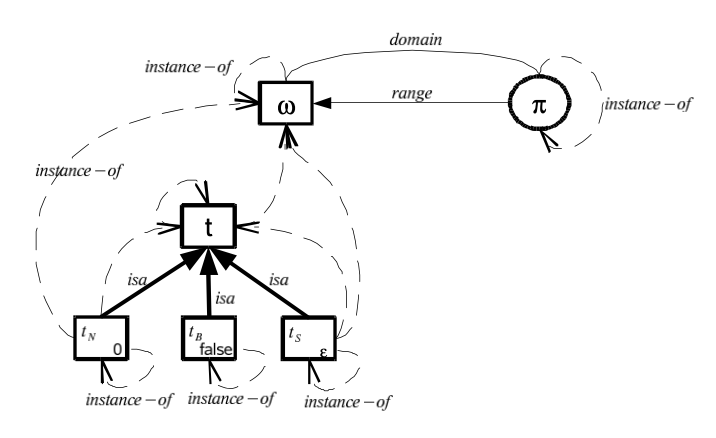
\includegraphics[width=0.7\textwidth]{img/etat_art/instanceOf.png}
\caption{Relations instanceOf réflexives explicites permettant la réification du type de propriété nom en une métapropriété de première classe P~\cite{Eng2007}}
\label{instanceOf}
\end{figure}

Cette méta-circularité est la propriété qui rend possible le \textit{bootstrapping} de MetaDONE. Grâce à elle, toute fonctionnalité de l'outil peut être définie comme un modèle conforme au même métamétamodèle, puis étendue sans modifier le code source~\cite{Eng2007}. GraSyLa lui-même est un DSML implémenté de cette façon~: ses spécifications sont des modèles concrets ordinaires du dépôt~\cite{techreportgrasylaversion2}.


En revanche, cette même propriété est source de défis techniques dès lors qu'il s'agit de \textbf{persister} le graphe du dépôt ou de le \textbf{charger en mémoire}.

% ---------------------------------------------------------------
\subsection{Conséquences pour la persistance}
\label{sec:graphes-persistance}
% ---------------------------------------------------------------

Les deux principales approches de persistance utilisées dans l'écosystème MDE ont été conçues en supposant des modèles essentiellement arborescents ou, au moins, acycliques~: elles rencontrent donc des difficultés structurelles face aux graphes cycliques de MetaL.

Le format XMI (\textit{XML Metadata Interchange}), standard OMG pour la persistance des modèles EMF, repose sur la structure hiérarchique de XML~\cite{specification2007omg}. XML est intrinsèquement arborescent~: chaque élément a exactement un parent, ce qui est incompatible avec un graphe contenant des cycles ou du partage (un nœud ayant plusieurs parents). Pour contourner cette limitation, XMI introduit un mécanisme de références croisées par identifiants (\textit{href})~: les objets partagés ou référencés de manière circulaire sont sérialisés une seule fois à leur point d'ancrage dans l'arbre, et référencés ailleurs par leur identifiant. Ce mécanisme fonctionne pour les modèles conventionnels mais présente des limites importantes dans le cas de MetaL~: la réflexivité totale implique que la quasi-totalité des items du métamétamodèle peuvent être à la fois la cible et la source de références circulaires, ce qui complexifie la détermination d'un ordre de sérialisation valide et impose une résolution de toutes les références lors du chargement avant de pouvoir utiliser le moindre objet. De surcroît, XMI nécessite le chargement intégral du fichier en mémoire avant de pouvoir en extraire une information partielle~\cite{steinberg2008emf}, ce qui le rend peu adapté aux grands modèles.

L'architecture du dépôt de MetaDONE est conçue pour être indépendante de la technologie de persistance sous-jacente~\cite{Eng2007}. L'implémentation courante repose sur OpenJPA qui mappe les objets Java vers un schéma relationnel~\cite{jpa2013}.

Ce mapping soulève un problème fondamental~: si les bases de données relationnelles représentent les données sous forme de tables et de clés étrangères sans difficulté particulière face aux références circulaires au niveau du stockage, les mécanismes de chargement objet-relationnel (ORM) y sont sensibles. Lorsqu'un ORM charge un objet, il doit décider comment charger ses références~: soit immédiatement (\textit{eager loading}), ce qui peut déclencher une cascade infinie en présence de cycles, soit à la demande (\textit{lazy loading}), ce qui reporte le problème à l'accès effectif à la référence. La résolution d'un graphe cyclique lors du chargement requiert donc un mécanisme explicite de détection des objets déjà en cours de chargement~: en garantissant qu'un identifiant donné correspond toujours à la même instance en mémoire, ce mécanisme --- connu sous le nom d'\textit{identity map} ou \textit{first-level cache} --- interrompt la récursion et retourne l'instance partiellement construite. La spécification JPA formalise ce comportement sous le terme \textit{persistence context}~\cite{jpa2013}.

Dans MetaDONE, cette contrainte est accentuée par le fait que les items séminaux de MetaL$_1$ --- qui forment les cycles les plus profonds du graphe --- sont nécessairement présents dans tout projet et constituent donc un point de passage obligé lors de chaque chargement du dépôt.

Les cycles structurels du graphe MetaL ne sont pas gérables par de simples heuristiques~: ils sont au cœur de la conception du langage. Toute stratégie d'optimisation des accès au dépôt de MetaDONE doit en tenir compte explicitement, que ce soit pour le chargement initial en mémoire, la mise en cache des objets fréquemment référencés, ou la stratégie de chargement différé des relations. Ces problématiques de persistance s'inscrivent dans un enjeu plus large de scalabilité du MDE, que la section suivante examine.

% ---------------------------------------------------------------
% ---------------------------------------------------------------
\section{Scalabilité en MDE}
\label{sec:scalabilite-mde}
% ---------------------------------------------------------------
% ---------------------------------------------------------------

Les sections précédentes ont établi que les modèles MDE sont fondamentalement des graphes, et que ceux de MetaDONE présentent la particularité d'être cycliques et denses par construction. Cette réalité structurelle s'inscrit dans un défi plus large que traverse l'ensemble de la communauté MDE depuis une décennie~: celui de la scalabilité. Le passage de modèles locaux de taille modeste à des écosystèmes de modèles interconnectés regroupant des millions d'éléments remet en cause les hypothèses fondatrices des outils MDE traditionnels~\cite{kolovos2013research}. Cette section passe en revue les principales dimensions de ce défi, en se concentrant sur celles qui sont directement pertinentes pour MetaDONE.

% ---------------------------------------------------------------
\subsection{Transformations et requêtes}
\label{sec:transfo-requetes}
% ---------------------------------------------------------------

Les transformations de modèles constituent le cœur opérationnel de la MDE~: elles permettent de générer automatiquement un modèle cible à partir d'un modèle source selon une définition de transformation~\cite{bezivin2005model}. Lorsque la taille des modèles augmente, les performances de ces transformations deviennent un enjeu critique.

Deux techniques complémentaires ont émergé comme réponses principales. La première est l'\textbf{incrémentalité}~: plutôt que de ré-exécuter une transformation sur l'ensemble du modèle à chaque modification, seules les parties affectées par le changement sont recalculées. Des outils comme EMF-IncQuery illustrent cette approche dans l'écosystème EMF~\cite{bergmann2010incremental}. La seconde est le \textbf{calcul différé} (\textit{lazy evaluation})~: les valeurs ne sont calculées qu'au moment où elles sont effectivement nécessaires, évitant ainsi le calcul prématuré de résultats qui ne seront jamais consultés.

Une piste de recherche plus récente consiste à adopter un paradigme \textit{réactif}, dans lequel un réseau de transformations définit des flux de données persistants. Chaque modification d'un modèle source propage automatiquement ses effets aux modèles dépendants, en n'activant que les calculs strictement nécessaires~\cite{cabot2012object}. Ce paradigme est particulièrement adapté aux environnements MetaCASE où les métamodèles et les modèles évoluent de concert.

% ---------------------------------------------------------------
\subsection{Modélisation collaborative}
\label{sec:model-collaborative}
% ---------------------------------------------------------------

La modélisation collaborative constitue une autre dimension de la scalabilité~: lorsque plusieurs utilisateurs travaillent simultanément sur un même modèle, la gestion de la cohérence et des conflits devient un problème d'envergure.

La plupart des outils MDE actuels n'atteignent pas la maturité des systèmes de gestion de versions de code source tels que Git ou SVN. EMFStore offre un support pour l'édition collaborative de modèles et de métamodèles EMF/Ecore, mais ne dispose pas de mécanisme de réconciliation basé sur les rôles et laisse à l'utilisateur ayant effectué le dernier commit la responsabilité de résoudre les conflits~\cite{koshima2016distributed}. MetaEdit+ recourt à un mécanisme de verrouillage fin (\textit{Smart Locks}) pour la gestion de la concurrence, mais les approches par verrou ne passent pas à l'échelle en équipes nombreuses~\cite{koshima2016distributed}. Des frameworks plus récents, comme DiCoMEF~\cite{koshima2016distributed}, proposent des architectures distribuées avec détection et réconciliation formalisées des conflits, mais restent au stade de la recherche.

La modélisation collaborative, bien que pertinente dans le domaine MDE, sort du périmètre de ce mémoire et ne sera pas davantage développée ici.

% ---------------------------------------------------------------
\subsection{Persistance de grands modèles}
\label{sec:persistance-modeles}
% ---------------------------------------------------------------

La persistance est la dimension de la scalabilité la plus directement liée aux objectifs de ce mémoire. Elle désigne la capacité d'un outil MDE à stocker et à charger efficacement des modèles de grande taille, en particulier lorsque ceux-ci présentent une structure complexe comme les graphes cycliques de MetaL.

% ---------------------------------------------------------------
\subsubsection{Limites de XMI}
\label{sec:limites-xmi}
% ---------------------------------------------------------------

Le format XMI (\textit{XML Metadata Interchange}) est le standard industriel de sérialisation des modèles EMF. Sa principale limite tient à sa nature même~: il impose un chargement et une désérialisation intégraux du fichier avant qu'une quelconque requête puisse être exécutée~\cite{steinberg2008emf}. Si la capacité mémoire des machines modernes atténue le problème pour des modèles de taille raisonnable, cette approche reste fondamentalement inefficace~: même une requête ponctuelle (par exemple, retrouver toutes les sous-classes d'un méta-objet donné) nécessite de parcourir l'intégralité du fichier, sans possibilité d'indexation ni d'accès incrémental. Le temps de chargement initial reste par ailleurs significatif pour les grands modèles, indépendamment de la mémoire disponible.

Comme détaillé à la section~\ref{sec:graphes-persistance}, XMI souffre en outre d'une incompatibilité structurelle avec les graphes cycliques~: étant fondé sur XML, il ne peut représenter qu'une arborescence, et doit donc recourir à des références croisées par identifiants pour simuler le partage ou les cycles. Pour les modèles réflexifs de MetaL, où la quasi-totalité des items séminaux sont à la fois instances et types de l'ensemble du graphe, ce mécanisme génère un grand nombre de références à résoudre lors du chargement, dont l'ordre de résolution doit être soigneusement géré.

Des travaux ont proposé de remplacer XMI par des formats binaires comme Google Protocol Buffers, pouvant réduire la taille des fichiers d'un facteur dix et améliorer la vitesse de chargement jusqu'à cent fois pour des modèles de grande taille~\cite{protobuf}. Ces approches restent cependant contraintes par la même hypothèse de chargement intégral en mémoire.

% ---------------------------------------------------------------
\subsubsection{Persistance par base de données avec OpenJPA}
\label{sec:persistance-openjpa}
% ---------------------------------------------------------------

Pour s'affranchir des limites des formats de fichiers, MetaDONE adopte une architecture de dépôt indépendante de la technologie de persistance sous-jacente, permettant de le connecter à différents backends~\cite{Eng2007}. L'implémentation principale repose sur OpenJPA, une implémentation de la Java Persistence API qui assure le mapping entre les objets Java du dépôt et un schéma relationnel.

Cette approche présente plusieurs avantages pour la scalabilité. D'abord, elle permet l'accès partiel aux données~: contrairement à XMI, une requête SQL ne nécessite pas de charger l'ensemble du modèle en mémoire, mais seulement les enregistrements pertinents. Ensuite, les bases de données relationnelles offrent des mécanismes d'indexation et d'optimisation des requêtes éprouvés sur de grandes volumétries.

Cependant, le mapping objet-relationnel (ORM) introduit un surcoût propre, particulièrement sensible dans le cas de MetaDONE. Plusieurs facteurs se conjuguent~:

\begin{itemize}
    \item \textbf{Multiplication des couches d'indirection.} La flexibilité totale de MetaL, qui permet à tout DataObject d'être simultanément objet, propriété et type, se traduit au niveau du schéma relationnel par une structure générique (table unique de \textit{DataObjects} avec jointures) plutôt que par des tables spécialisées par type de méta-objet. Englebert et Heymans notent explicitement que le coût de cette flexibilité est la multiplication des couches d'indirection~\cite{Eng2007}, dont l'impact sur les performances devait être évalué pour les usages avancés.

    \item \textbf{Chargement des cycles.} Comme exposé à la section~\ref{sec:graphes-persistance}, le chargement d'objets appartenant à des cycles de la relation \texttt{instanceOf} requiert un mécanisme d'\textit{identity map}~: chaque objet partiellement construit doit être enregistré dans un cache local avant que ses références soient résolues, afin d'interrompre la récursion et de retourner l'instance déjà en cours de construction~\cite{jpa2013}. Sans ce mécanisme, le chargement diverge infiniment.

    \item \textbf{Stratégie de chargement des relations.} En JPA, les relations entre entités peuvent être chargées immédiatement (\textit{eager}) ou à la demande (\textit{lazy})~\cite{jpa2013}. Pour un graphe cyclique, le chargement immédiat provoque une cascade potentiellement infinie~; le chargement différé reporte les accès à la base de données au moment de la première traversée de chaque relation. Il en résulte le problème dit du \textit{N+1 queries}~: une itération sur $N$ objets peut alors déclencher $N$ requêtes supplémentaires si les relations ne sont pas pré-chargées par lot. Ce surcoût ne se manifeste toutefois qu'en présence d'accès effectifs à la base, et reste donc latent pour les charges essentiellement CPU-bound.

    \item \textbf{Absence d'indexation sémantique.} Les requêtes globales sur le modèle (par exemple, retrouver toutes les instances d'un méta-objet donné, ou l'ensemble des sous-types d'un type) nécessitent des jointures sur plusieurs tables et peuvent s'avérer coûteuses. Un serveur d'indexation dédié surveillant le dépôt et maintenant des index sémantiques permettrait de répondre à ces requêtes en temps constant~\cite{kolovos2013research}.
\end{itemize}

La persistance par base de données est la solution la plus adaptée à la nature réflexive et cyclique des modèles MetaL. Elle reste néanmoins sujette à des surcoûts caractéristiques --- couches d'indirection, gestion des cycles au chargement, problème du N+1 et absence d'indexation sémantique --- qui constituent précisément les points d'attention de ce mémoire.

% ---------------------------------------------------------------
% ---------------------------------------------------------------
\section{Synthèse et question de recherche}
\label{sec:synthese-question}
% ---------------------------------------------------------------
% ---------------------------------------------------------------

La MDE place les modèles au cœur du processus de développement logiciel, et les outils MetaCASE constituent la réponse la plus flexible à ce paradigme : en stockant le méta-modèle comme donnée modifiable plutôt qu'en dur dans le code, ils permettent d'adapter l'environnement de modélisation à n'importe quel domaine. Dans ce panorama, MetaDONE se distingue de ses concurrents — MetaEdit+, WebGME et ConceptBase — par la combinaison unique de trois propriétés fondamentales : un nombre illimité de niveaux d'abstraction, un metamodelling non-strict permettant aux relations de traverser les niveaux, et une réflexivité totale. ConceptBase partage les deux premières mais n'offre qu'une réflexivité partielle ; MetaEdit+ et WebGME, ancrés dans la tradition strictement OMG, ne possèdent aucune des trois. Ces propriétés lui confèrent une expressivité difficile à égaler, mais au prix d'une complexité structurelle accrue.

Cette complexité se manifeste concrètement dans la représentation des données : les modèles MetaL forment des graphes denses contenant des cycles structurels issus de la réflexivité. Ces cycles sont au cœur de la conception du langage et rendent inadaptées les hypothèses d'acyclicité sur lesquelles reposent la plupart des outils de persistance MDE. XMI, fondé sur une structure XML arborescente, en est l'illustration directe. OpenJPA, solution retenue par MetaDONE, contourne ce problème mais introduit ses propres surcoûts : multiplication des couches d'indirection, gestion des cycles au chargement, problème du N+1 et absence d'indexation sémantique.

L'ensemble de ces observations converge vers deux questions de recherche complémentaires~:
\begin{description}
    \item[QR1.] Quels sont les goulots d'étranglement réels de MetaDONE lorsque la taille des modèles manipulés croît~?
    \item[QR2.] Dans quelle mesure ces goulots peuvent-ils être réduits sans renoncer aux principes architecturaux du framework — en particulier la réflexivité de MetaL et le Design by Contract~?
\end{description}
Le chapitre suivant présente l'architecture interne de MetaDONE qui constitue le cadre dans lequel les optimisations ont été identifiées et mises en œuvre.
\chapter{Architecture de MetaDONE}
\label{chap:architecture}

L'architecture de l'outil MetaDONE repose sur une structure en trois couches : la couche présentation (\texttt{metadone\_bundle\_client}), la couche logique métier (\texttt{metadone\_bundle\_metabusiness}) et la couche repository (\texttt{metadone\_bundle\_repository}). Afin de garantir une grande modularité et extensibilité, MetaDONE s'appuie sur Eclipse Equinox, une implémentation du standard OSGi. Ce framework permet de découper l'application en composants dynamiques et indépendants appelés bundles. L'un des atouts majeurs de cette architecture est la possibilité d'installer, de démarrer, de mettre à jour ou d'arrêter ces modules au moment de l'exécution, sans nécessiter d'interruption de service.

Dans les sous-sections suivantes, nous développerons les langages de modélisation de MetaDONE, MetaL$_1$ et MetaL$_2$, le pattern \emph{Design by Contract} utilisé dans toute l'application, ainsi chacun des bundles présentés à la figure~\ref{fig:bundles-overview}.

\paragraph{Note sur l'usage d'outils d'assistance.}
Les figures représentant les bundles MetaDONE (figures~\ref{fig:bundles-overview}, \ref{bundle-client}, \ref{bundle-MB}, \ref{bundle-repo} et~\ref{bundle-common}) ainsi que le diagramme du langage MetaL$_2$ (figure~\ref{fig:metaL2}) ont été générées à partir de spécifications PlantUML produites avec l'assistance d'un modèle de langage. Chaque diagramme a été relu et corrigé manuellement pour assurer la fidélité au code source.

\begin{figure}[h]
\centering
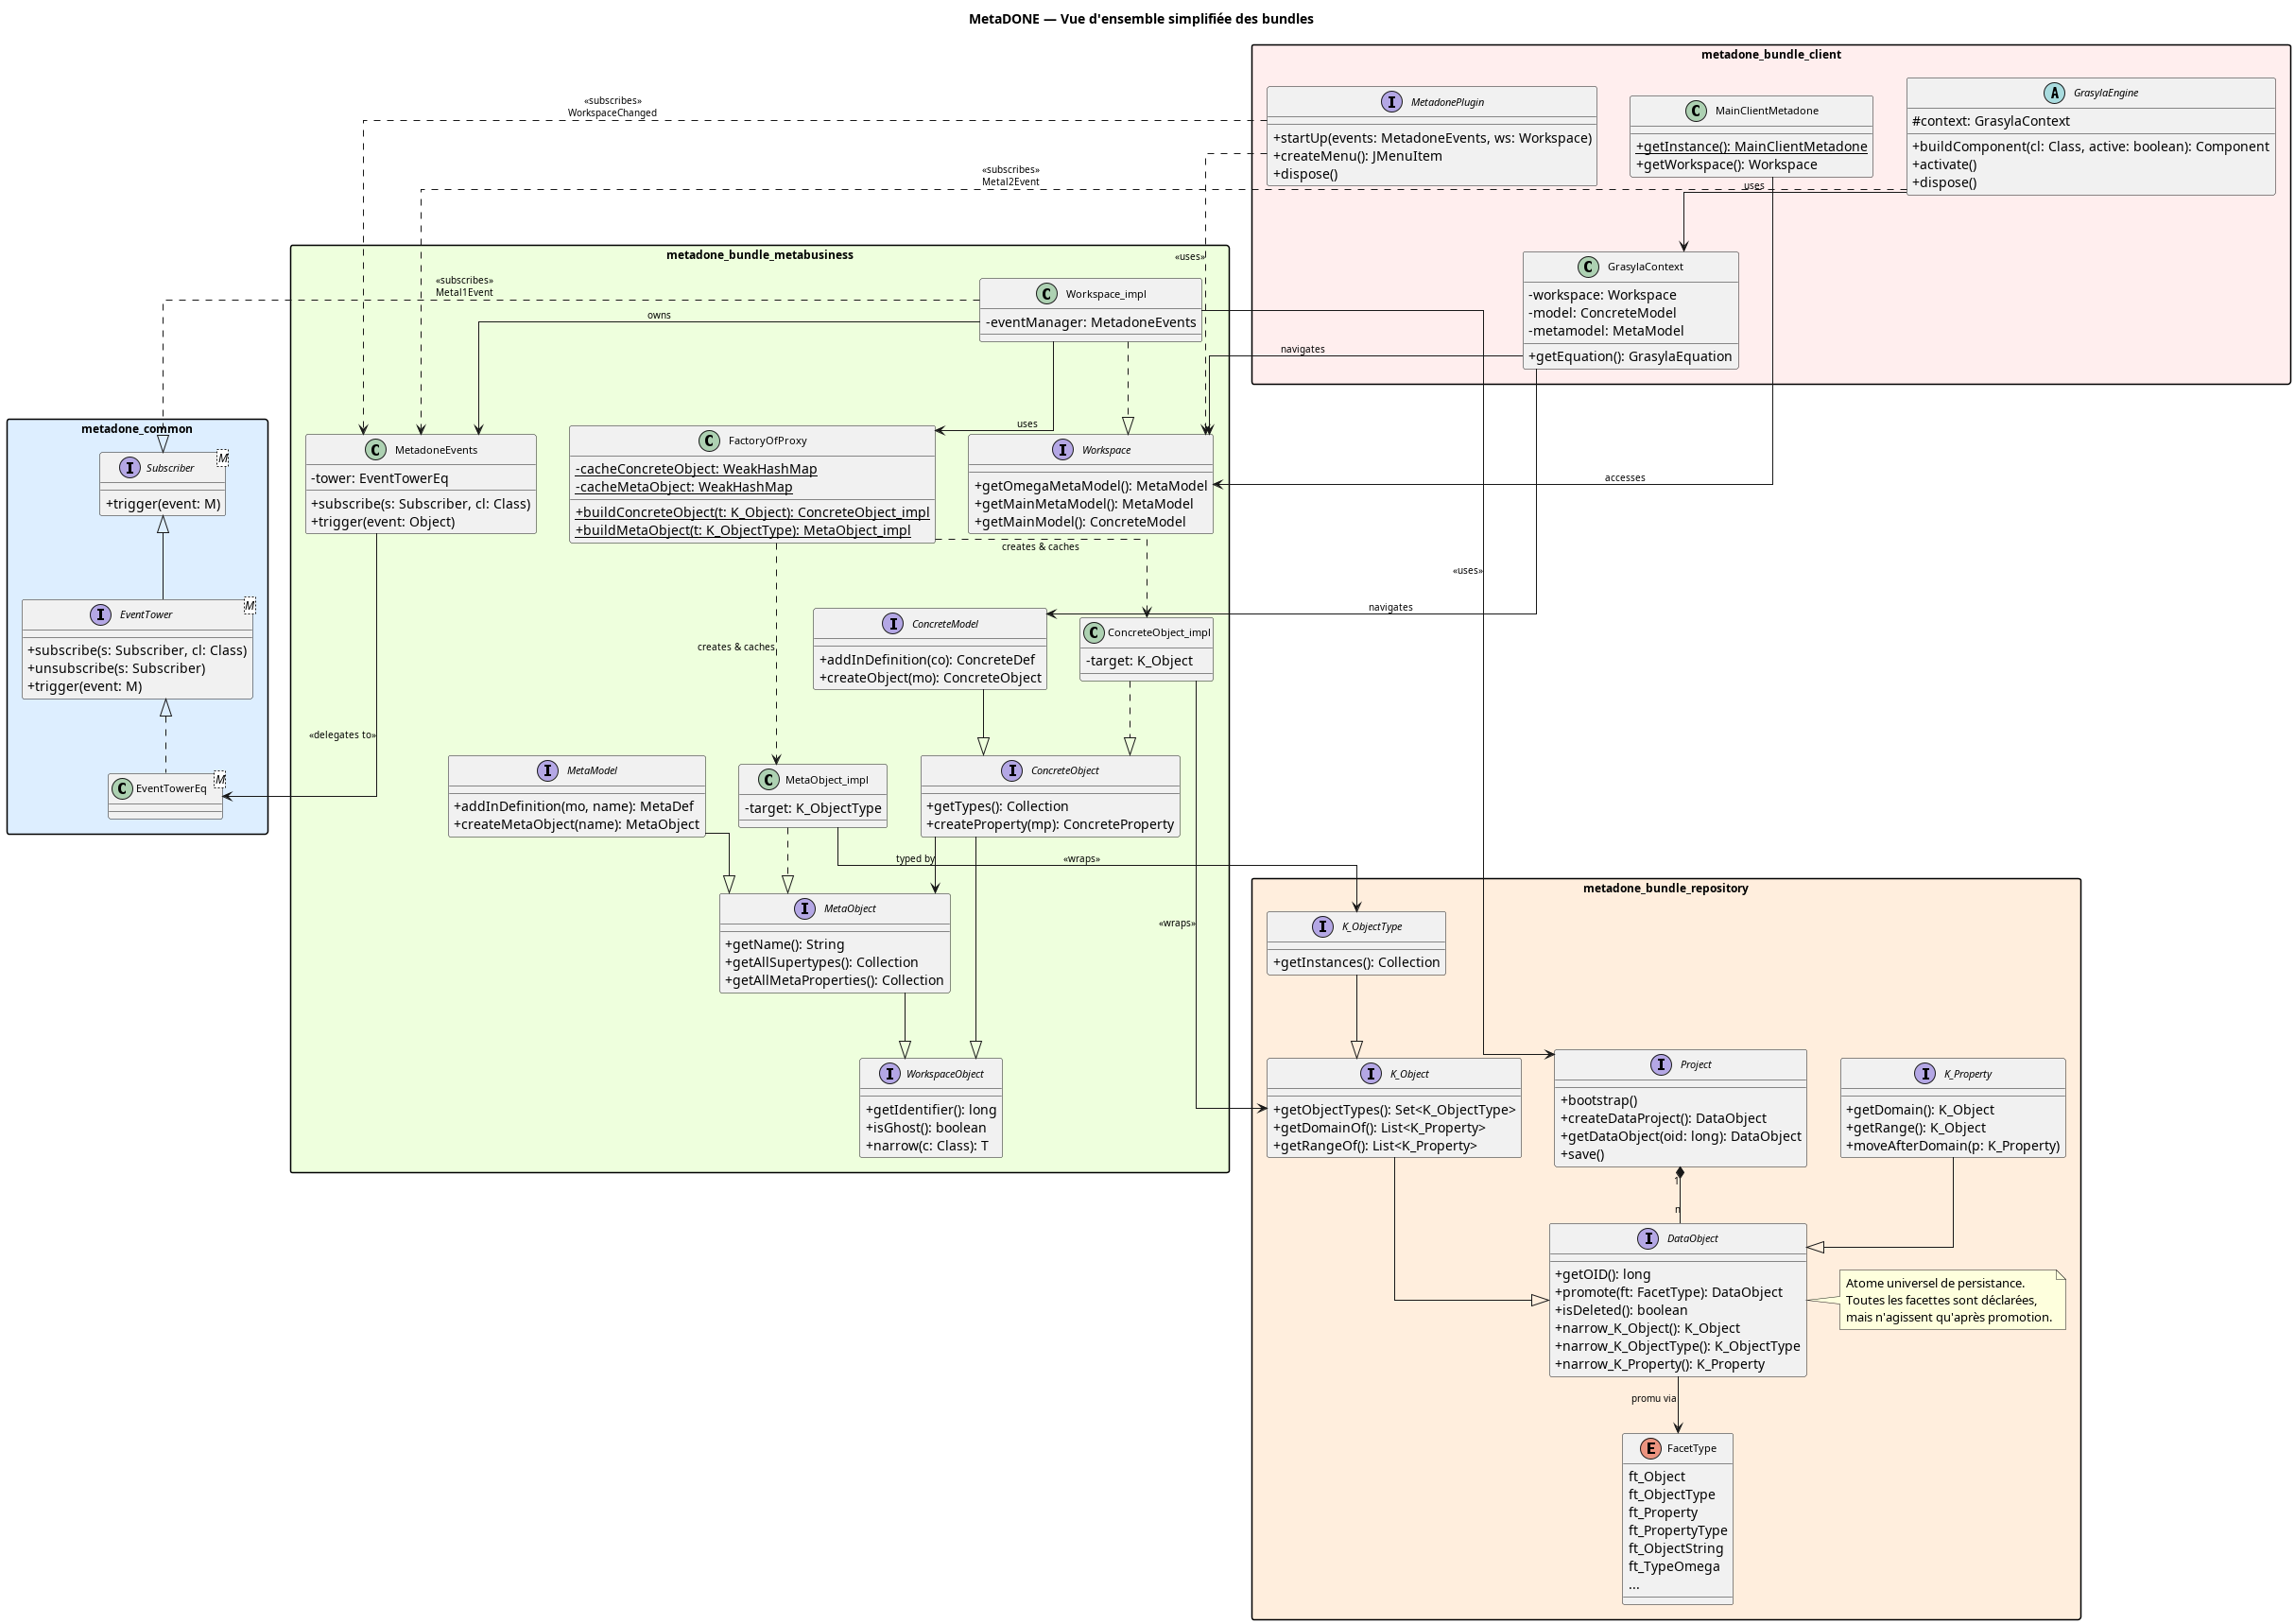
\includegraphics[width=0.8\textwidth]{img/architecture/bundles-overview.png}
\caption{Bundles MetaDONE}
\label{fig:bundles-overview}
\end{figure}

% ---------------------------------------------------------------
% ---------------------------------------------------------------
\section[MetaL$_1$ et MetaL$_2$]{MetaL$_1$ et MetaL$_2$ : les deux niveaux de MetaDONE}
\label{sec:metal1-2}
% ---------------------------------------------------------------
% ---------------------------------------------------------------

MetaDONE repose sur une architecture à deux spécifications complémentaires, inspirée du standard MOF (voir section~\ref{sec:dsl-dsml}). MetaL$_1$ constitue le noyau formel du framework : il définit un ensemble minimal de construits de bas niveau sur lequel tout le reste est bâti. MetaL$_2$ est le langage de modélisation construit entièrement sur ce substrat ; il se décline en deux couches d'instanciation : la couche méta-modèle (niveaux M2 et M3) et la couche concrète (niveau M1). Ces deux spécifications structurent l'ensemble du framework et constituent le vocabulaire central que l'on retrouve à travers tous les bundles.

% ---------------------------------------------------------------
\subsection{MetaL$_1$ : le noyau formel}
\label{sec:metal1}
% ---------------------------------------------------------------


MetaL$_1$ est la spécification formelle du dépôt de MetaDONE. Elle se réduit à un unique construit, le \texttt{DataObject}, et à un ensemble fini de \emph{facettes} (\texttt{K\_Object}, \texttt{K\_ObjectType}, \texttt{K\_Property}, \texttt{K\_PropertyType}, ainsi que les facettes de type primitif) qu'un \texttt{DataObject} peut acquérir cumulativement~\cite{englebert_metal1}. À ce niveau, aucune notion de \og méta-objet \fg{} ni d'\og objet concret \fg{} n'existe encore : ces sémantiques sont l'apanage de MetaL$_2$, qui se construit sur le substrat de MetaL$_1$. Dans MetaDONE, MetaL$_1$ est implémenté par le bundle \texttt{metadone\_bundle\_repository} ; MetaL$_2$ n'en est qu'un client.


\subsection{MetaL$_2$ : la couche méta-modèle (M2/M3)}
\label{sec:metal2}

MetaL$_2$ est la couche de description. Elle permet de définir la structure d'un domaine : quels types d'objets existent, quels attributs ils portent et quelles relations les lient. Les concepts fondamentaux de cette couche sont décrits ci-dessous et sont représentés à la figure~\ref{fig:metaL2}.

Un \texttt{MetaObject} représente un type du domaine modélisé, analogue à une classe dans un langage orienté objet. Il supporte l'héritage multiple via les relations de sous-typage (\texttt{getAllSupertypes()}, \texttt{getAllSubtypes()}) et expose l'ensemble de ses attributs hérités (\texttt{getAllMetaProperties()}).

Un \texttt{MetaModel} est un espace de noms regroupant des \texttt{MetaObject}. Il joue le rôle de \emph{package} ou de \emph{namespace} et fournit les opérations de création des éléments qu'il contient. L'appartenance d'un \texttt{MetaObject} à un \texttt{MetaModel} est matérialisée par une instance de \texttt{MetaDef}, qui enrichit cette relation de trois métadonnées~: un booléen \texttt{canNotBeShared} interdisant le partage de l'objet entre plusieurs modèles ; un booléen \texttt{isDependentOn} précisant si l'objet doit être supprimé en cascade lors de la suppression du modèle ; et un booléen \texttt{isHidden} permettant de masquer les concepts techniques dans l'interface utilisateur. %La spécification formelle~\cite{englebert_metal2} mentionne une quatrième propriété (\texttt{nickname}, pour renommer localement un méta-objet) qui n'a pas été implémentée dans la version actuelle de MetaDONE.

Une \texttt{MetaProperty<T>} est un attribut typé d'un \texttt{MetaObject}. Elle porte la cardinalité, le type de valeur attendu et, le cas échéant, une liste de valeurs énumérées autorisées.

Un \texttt{MetaRole} est une relation binaire dirigée entre deux \texttt{MetaObject} : un domaine et un codomaine (\emph{range}). Il précise la cardinalité de la relation (1-1, 1-N, N-1, N-N) et si les collections aux deux extrémités sont ordonnées. Chaque extrémité porte un nom de navigation (\texttt{getDomainName()}, \texttt{getRangeName()}).

Il convient de souligner que \texttt{MetaProperty}, \texttt{MetaRole} et \texttt{MetaModel} héritent tous de \texttt{MetaObject}: ils sont eux-mêmes des méta-objets, et peuvent à ce titre participer aux mêmes mécanismes de typage et de réflexivité.

\begin{figure}[h]
\centering
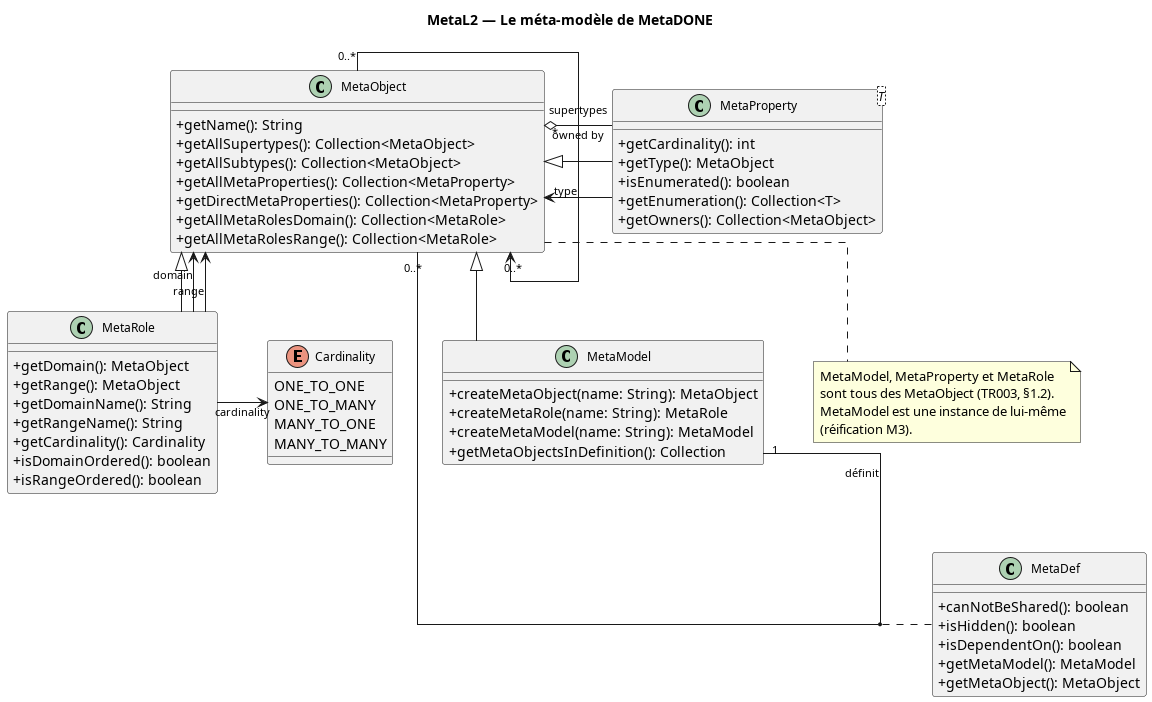
\includegraphics[width=0.9\textwidth]{img/architecture/metal2.png}
\caption{Langage de modélisation MetaL$_2$}
\label{fig:metaL2}
\end{figure}

% ---------------------------------------------------------------
\subsection{MetaL$_2$ : la couche concrète (M1)}
\label{sec:couche-concrete}
% ---------------------------------------------------------------

La couche concrète est la couche d'instanciation de MetaL$_2$. Elle contient les objets effectivement manipulés lors de l'exécution d'un outil construit avec MetaDONE. Chaque concept y est le miroir concret de son homologue de la couche méta-modèle : là où la couche méta-modèle emploie les construits de type de MetaL$_1$ (\texttt{K\_ObjectType}, \texttt{K\_PropertyType}), la couche concrète repose sur les construits d'instance (\texttt{K\_Object}, \texttt{K\_Property}).

Un \texttt{ConcreteObject} est une instance d'un ou plusieurs \texttt{MetaObject}. Il peut posséder plusieurs types simultanément, potentiellement issus de méta-modèles différents (\texttt{getTypes()}, \texttt{getType(MetaModel)}). Un \texttt{ConcreteModel} est un conteneur de \texttt{ConcreteObject}, instance d'un \texttt{MetaModel}. De même qu'un \texttt{MetaDef} lie un \texttt{MetaObject} à son méta-modèle, un \texttt{ConcreteDef} lie un objet concret à son modèle.

Une \texttt{ConcreteProperty<T>} est la valeur effective d'une \texttt{MetaProperty} pour un \texttt{ConcreteObject} donné. Un \texttt{ConcreteRole} est le lien concret entre deux \texttt{ConcreteObject}, instance d'un \texttt{MetaRole}.

% ---------------------------------------------------------------
\subsection{Le \texttt{Workspace} comme point d'entrée}
\label{sec:workspace}
% ---------------------------------------------------------------

Le \texttt{Workspace} est l'interface racine qui donne accès aux deux couches. Il expose systématiquement deux instances de chaque niveau :

\begin{itemize}
    \item \texttt{getOmegaMetaModel()} et \texttt{getOmegaModel()} : le méta-modèle et le modèle prédéfinis par MetaDONE, en lecture seule, qui contiennent les types primitifs (String, Integer, Float, Boolean, Char) ainsi que les méta-types du framework.
    
    \item \texttt{getMainMetaModel()} et \texttt{getMainModel()} : le méta-modèle et le modèle définis par l'utilisateur ou le plugin, dans lesquels sont créés les types du domaine et leurs instances.
\end{itemize}

% ---------------------------------------------------------------
\subsection{Un premier regard sur la réflexivité}
\label{sec:reflexivite-intro}
% ---------------------------------------------------------------

Un trait caractéristique de cette architecture est que \texttt{MetaProperty}, \texttt{MetaRole} et \texttt{MetaModel} héritent tous de \texttt{MetaObject}, et que symétriquement \texttt{ConcreteProperty}, \texttt{ConcreteRole} et \texttt{ConcreteModel} héritent tous de \texttt{ConcreteObject}. Un méta-modèle est donc lui-même un méta-objet, et un modèle concret est lui-même un objet concret : ils peuvent avoir des types, des propriétés et participer à des rôles au même titre que n'importe quel élément de MetaL$_2$.  Cette propriété, dit \emph{réflexive}, permet à MetaDONE de se décrire lui-même avec ses propres outils : le méta-modèle Omega décrit les concepts de MetaL$_2$ (\texttt{MetaObject}, \texttt{MetaRole}, etc.) comme des \texttt{MetaObject} ordinaires. Les implications de cette réflexivité sur l'architecture et les performances seront développées en section~\ref{sec:reflexivite}.

% ---------------------------------------------------------------
\section{Principes de développement}
% ---------------------------------------------------------------

Avant de décrire les bundles, il convient de présenter les principes architecturaux qui structurent de façon uniforme toute l'implémentation de MetaDONE.

% ---------------------------------------------------------------
\subsection{Design by Contract}
\label{sec:dbc}
% ---------------------------------------------------------------

MetaDONE applique systématiquement le patron \emph{Design by Contract} dans l'ensemble de ses couches d'implémentation. Ce
patron repose sur une séparation stricte entre les responsabilités des
méthodes publiques et celles des méthodes privées.

Chaque opération est donc décomposée en deux niveaux :
\begin{enumerate}
    \item \textbf{La méthode publique} constitue la frontière du contrat.
    Elle valide de façon défensive l'ensemble des préconditions de son
    appelant : nullité des arguments, cohérence des états, unicité des
    éléments. En cas de violation, elle lève une \texttt{BadPreCondition} (ou sa spécialisation \texttt{NullArgument}).
    Une fois toutes les préconditions satisfaites, elle délègue le travail effectif à la méthode privée correspondante, conventionnellement préfixée par le caractère \texttt{\_}.

    \item \textbf{La méthode privée} opère sous hypothèse que les
    préconditions ont déjà été vérifiées par son appelant et utilise des \texttt{assert} Java pour documenter et vérifier ses invariants en mode débogage. Ces assertions peuvent être désactivées en production
    sans aucun coût fonctionnel.
\end{enumerate}

\paragraph{Exemple 1 — \texttt{ConcreteObject\_impl.getType()}.}
La méthode publique \texttt{getType} ne fait que vérifier que son
argument n'est pas nul avant de déléguer à \texttt{\_getType} :

\begin{lstlisting}[language=Java]
// Methode publique : verification defensive
public MetaObject getType(MetaModel metamodel) throws BadPreCondition {
    NullArgument.check(metamodel);   // leve BadPreCondition si null
    return _getType(metamodel);      // delegation au prive
}

// Methode privee : assertions internes
private MetaObject _getType(MetaModel metamodel) {
    // metamodel != null garanti par l'appelant public
    final Set<MetaObject> allTypesOfThis = new HashSet<MetaObject>();
    for (final K_ObjectType type : target.getObjectTypes()) { ... }
    assert allTypesOfThis.size() > 0;  // invariant verifie en debug
    ...
}
\end{lstlisting}

\paragraph{Exemple 2 — \texttt{MetaObject\_impl.createMetaProperty()}.}
La méthode publique effectue plusieurs validations sémantiques avant de
déléguer. Le commentaire \texttt{// OK. preconditions are verified.} est
une convention explicite utilisée dans tout le code pour marquer la
transition :

\begin{lstlisting}[language=Java]
// Methode publique : validations metier
public MetaPropertyExt<T> createMetaProperty(
        Class<T> type, String name,
        int cardinality, MetaModel metamodel) throws BadPreCondition {

    precondition_createMetaObject(metamodel, name, null);

    if (!workspace.getProject().isPrimitiveType(ptype))
        throw new BadPreCondition(
            "The type of a metaproperty must denote a primitive type");

    if (!(cardinality >= 0 || cardinality == MetaProperty.INFINITY))
        throw new BadPreCondition(
            "The cardinality of the metaproperty is not correct");

    // OK. preconditions are verified.
    return _createMetaProperty(name, cardinality, ptype, metamodel);
}

// Methode privee : logique d'implementation, assertions internes
private MetaPropertyExt<?> _createMetaProperty(
        String name, int cardinality,
        K_ObjectType type, MetaModel metamodel) throws BadPreCondition {
    assert name != null && type != null && metamodel != null;
    ...
}
\end{lstlisting}

La classe \texttt{NullArgument} (dans \texttt{metadone\_common/metadone.exception}) est l'outil principal de la validation défensive. Sa méthode statique \texttt{check(Object...)} accepte un nombre variable d'arguments et lève une \texttt{NullArgument extends BadPreCondition} dès que l'un d'eux est
nul, évitant la répétition de blocs \texttt{if (x == null)} dans chaque
méthode publique.

Ce patron présente plusieurs avantages dans une architecture réflexive comme MetaDONE. Premièrement, il concentre la validation à la frontière de l'API publique : tout invariant du modèle ne peut être mis en défaut que par un appelant externe, et la violation est détectée au plus tôt, à l'entrée même du système. Deuxièmement, il permet de désactiver les \texttt{assert} en production pour réduire le coût des vérifications internes, tout en les conservant actifs lors des tests. Enfin, la convention de nommage \texttt{\_methode} pour les méthodes privées rend immédiatement visible, à la lecture du code, quelle couche
porte la responsabilité de la validation.


\section{Bundle \texttt{metadone\_bundle\_client}}

Le bundle \texttt{metadone\_bundle\_client} constitue la couche de présentation de MetaDONE. Il regroupe l'ensemble des composants responsables de l'interaction avec l'utilisateur : interface graphique Swing, moteur de rendu, système de plugins, parsers et importeurs. C'est le point d'entrée de l'application ; ses principaux composants sont représentés à la figure~\ref{bundle-client}.

\begin{figure}[h]
\centering
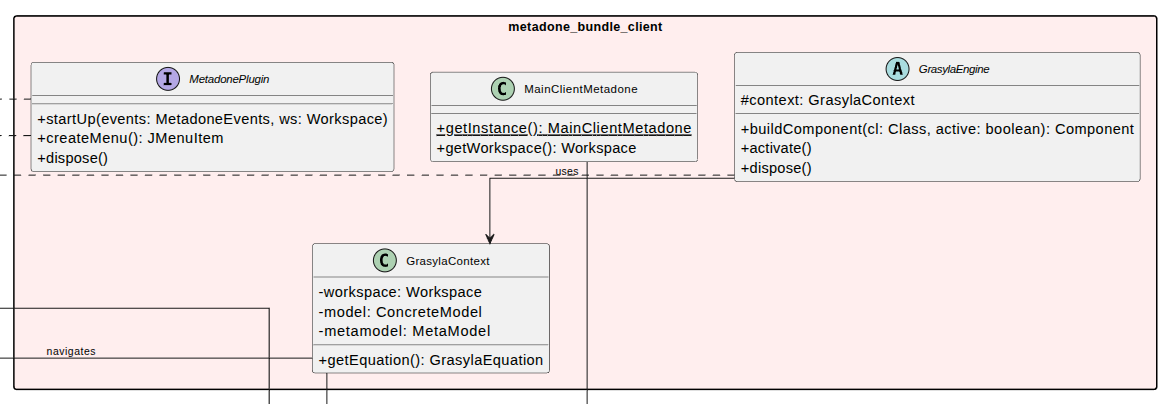
\includegraphics[width=0.9\textwidth]{img/architecture/bundle-client.png}
\caption{Bundle client}
\label{bundle-client}
\end{figure}

%\subsection{Intégration OSGi et point d'entrée}

%Conformément au modèle de composants OSGi, le bundle présente une classe \texttt{MetadoneActivator} qui instancie deux trackers : \texttt{ClientBusinessTracker} surveille l'apparition du service \texttt{Workspace} dans le registre OSGi, et \texttt{PluginTracker} détecte dynamiquement les plugins enregistrés par d'autres bundles.

\subsection{Système de plugins}

MetaDONE adopte une architecture orientée plugins pour garantir son extensibilité. Tout plugin implémente l'interface \texttt{MetadonePlugin}, qui impose quatre responsabilités : fournir un nom, contribuer un élément de menu Swing, réagir aux changements de workspace via \texttt{startUp} et libérer ses ressources via \texttt{dispose}.

La classe abstraite \texttt{AbstractMetadonePlugin} fournit une implémentation de base : elle souscrit automatiquement aux événements \texttt{WorkspaceChanged} afin de maintenir sa référence vers le workspace courant à jour. Chaque plugin est déployé dans son propre bundle OSGi et expose un \texttt{AbstractPluginActivator} qui l'enregistre dans le
registre de services au démarrage. Le \texttt{PluginTracker} du bundle client détecte ces enregistrements et intègre les menus correspondants dans l'interface principale sans nécessiter de recompilation ni de redémarrage de l'application.

\subsection{Abstraction de rendu}

Pour découpler la logique d'affichage des technologies d'interface graphique sous-jacentes, le bundle introduit une abstraction de rendu structurée en trois interfaces centrales.
\begin{itemize}
    \item L'interface \texttt{Context} encapsule l'environnement d'évaluation d'une vue : workspace courant, modèle concret, méta-modèle et table de variables.
    \item L'interface \texttt{Engine} représente un composant capable de produire un élément d'interface à partir d'un contexte donné. Sa méthode \texttt{buildComponent(Class<C>, boolean)} est générique : selon que l'on passe \texttt{JComponent.class} ou \texttt{Widget.class} (NetBeans Visual Library), le même engine produit un widget Swing ou un nœud de graphe interactif. 
    \item Enfin, l'interface \texttt{Component<C>} encapsule le résultat produit et maintient un lien vers l'engine l'ayant construit.
\end{itemize}
Les engines s'organisent en arbre parent-enfant : un engine composite gère le cycle de vie de ses enfants (activation, disposition) de façon transparente.

\subsection{Le langage GraSyLa}
\label{sec:grasyla}

Présenté brièvement en section~\ref{sec:dsl-dsml}, GraSyLa (\emph{Graphical Symbolic Language}) est un DSML intégré au bundle client, dont le rôle est de décrire de façon déclarative comment visualiser les objets d'un modèle. Plutôt que de coder en dur la représentation graphique de chaque type d'objet, un plugin ou un utilisateur avancé rédige des \emph{équations GraSyLa} qui associent des motifs sur le modèle à des structures visuelles.

Une équation GraSyLa a la forme générale \texttt{motif => expression}, où le membre gauche désigne un \texttt{MetaObject} du métamodèle (filtrant par typage les objets concrets concernés) et le membre droit décrit la structure graphique à produire : boîtes imbriquées, libellés, arbres, arêtes de graphe, images SVG, etc. Ce mécanisme permet à un même objet d'être affiché différemment selon le
contexte dans lequel il est visualisé.

La structure formelle d'un script GraSyLa est décrite par son méta-modèle, présenté à la figure~\ref{grasyla}~\cite{techreportgrasylaversion2}. Ce méta-modèle est lui-même exprimé à l'aide des concepts de MetaL$_2$, illustrant ainsi la réflexivité de MetaDONE : le framework décrit son propre langage de visualisation avec ses propres
outils de méta-modélisation.

\begin{figure}[tp]
\centering
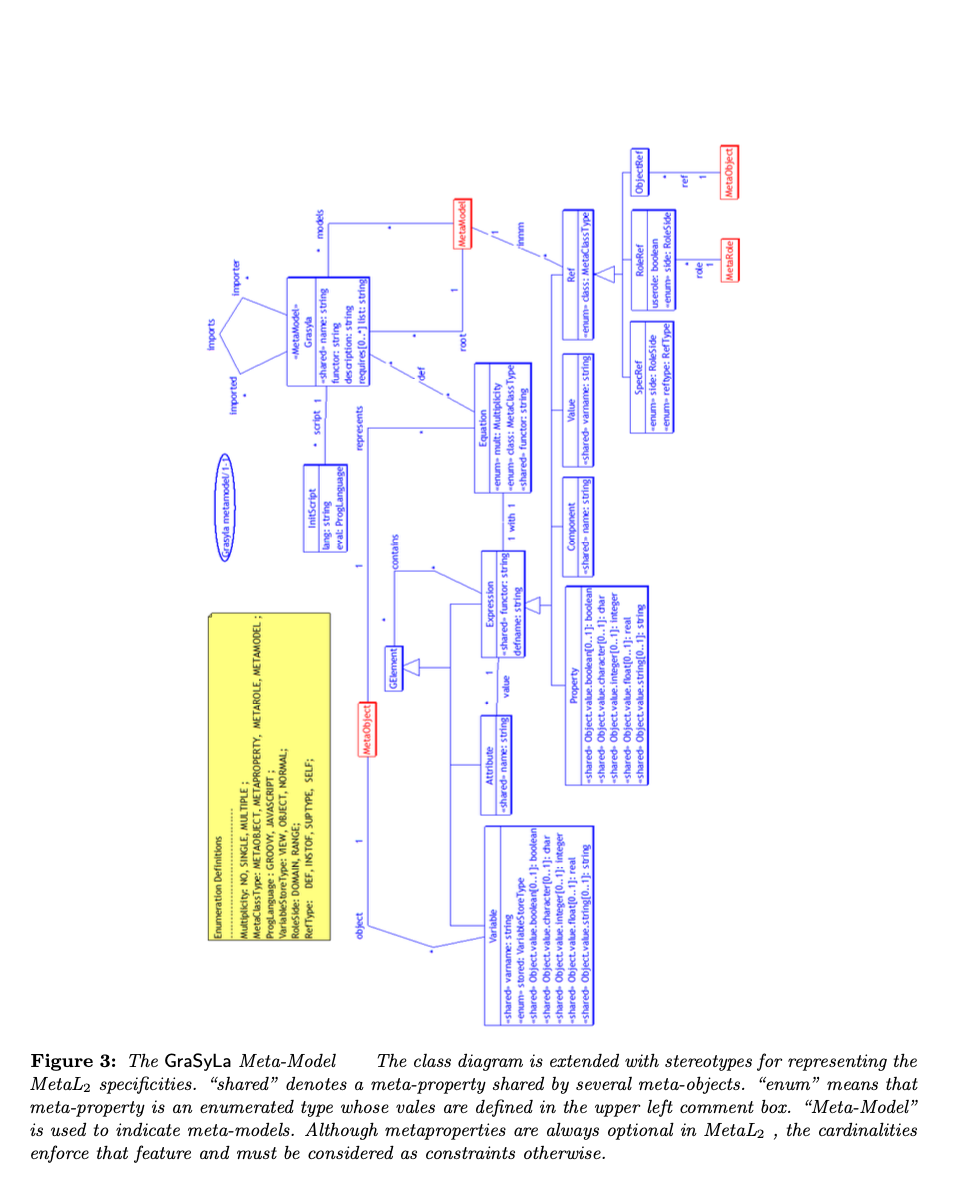
\includegraphics[width=\textwidth]{img/architecture/grasyla.png}
\caption{Méta-modèle de GraSyLa, exprimé en MetaL$_2$~\cite{techreportgrasylaversion2}}
\label{grasyla}
\end{figure}

Un script GraSyLa (\texttt{GrasylaMetamodel}) regroupe un ensemble d'équations (\texttt{Equation}) et un script d'initialisation optionnel (\texttt{InitScript}). Chaque équation possède un membre gauche
(\emph{LHS}) qui référence un \texttt{MetaObject} via la relation
\texttt{represents}, et un membre droit (\emph{RHS}) constitué d'un
arbre d'\texttt{Expression}. Cet arbre peut contenir des composants
(\texttt{Component}), des attributs visuels (\texttt{Attribute}), des
variables (\texttt{Variable}) et des propriétés (\texttt{Property}).
Les références au modèle sont typées : \texttt{ObjectRef} pointe vers
un objet concret, \texttt{RoleRef} vers un rôle, et \texttt{SpecRef}
vers une spécification.


L'interprétation d'un script GraSyLa repose sur deux composants principaux. Le \texttt{GrasylaContext} maintient l'état d'évaluation : workspace, modèle courant, méta-modèle, variables locales et équation sélectionnée. Le \texttt{GrasylaInterpreter}, qui étend \texttt{GrasylaEngine} et implémente \texttt{EngineInterpreter}, sélectionne la meilleure équation pour un objet donné puis délègue la construction du composant graphique aux engines spécialisés.

Ces engines spécialisés sont regroupés en plusieurs familles~:
\begin{itemize}
    \item \textbf{Engines Swing} (\texttt{JBoxEngine}, \texttt{JTreeEngine}, \texttt{JTableEngine}, \texttt{JComboBoxEngine}, etc.) : produisent des composants \texttt{JComponent} pour l'affichage dans des panneaux Swing classiques.
    \item \textbf{Engines Visual Library} (\texttt{GraphEngine}, \texttt{VLBoxEngine}, \texttt{VLEdgeEngine}, \texttt{VLShapeEngine}, etc.) : produisent des widgets NetBeans Visual Library pour l'affichage de graphes interactifs avec ancres, routeurs et formes personnalisées.
    \item \textbf{Engines logiques} : \texttt{IfEngine}, \texttt{GuardEngine}, \texttt{MatchEngine}, \texttt{OrEngine}, \texttt{NotEngine} permettent d'exprimer des conditions sur le modèle directement dans le script.
    \item \textbf{Engines de structure} : \texttt{ListEngine}, \texttt{GroupEngine}, \texttt{ReduceEngine}, \texttt{HeadEngine}, \texttt{TailEngine} permettent d'itérer sur des collections d'objets ou de rôles.
    \item \textbf{Engines de référence} (\texttt{CORefObjectEngine}, \texttt{MORefObjectEngine}, \texttt{MRRefRoleEngine}) : naviguent dans le modèle pour accéder aux objets concrets, aux méta-objets ou aux
    rôles référencés.
    \item \textbf{Engines de valeur} (\texttt{ValueEngine},
    \texttt{UpdaterEngine}, \texttt{MutableValue}) : lisent et modifient les propriétés d'un objet concret, propageant les changements via le système d'événements.
\end{itemize}

GraSyLa souscrit au système d'événements de MetaDONE : lorsqu'un objet est modifié ou supprimé, les engines actifs se rafraîchissent automatiquement sans intervention explicite du code applicatif.

\subsection{Dialogues Swing}

Le bundle fournit un ensemble de dialogues Swing couvrant les opérations courantes sur le méta-modèle et le modèle concret.

Les \emph{browsers} \texttt{BrowserMetal2} et \texttt{BrowserMetal1} présentent respectivement le méta-modèle (couche M2) et le modèle concret (couche M1) sous forme d'arbres navigables. Chaque nœud de l'arbre correspond à un concept précis : \texttt{NodeRoot\_MetaModel}, \texttt{NodeRoot\_MetaObject}, \texttt{NodeRoot\_MetaRole} pour M2 ; \texttt{NodeTypes}, \texttt{NodeProperties}, \texttt{NodeDomain}, \texttt{NodeInstances} pour M1.

Les éditeurs de méta-objets (\texttt{PanelMetaModel}, \texttt{PanelMetaObject}, \texttt{PanelMetaProperty}, \texttt{PanelMetaRole}) permettent de créer et modifier les éléments du méta-modèle. Pour les objets concrets, le \texttt{DialogConcreteObject} est construit dynamiquement par un \texttt{Builder} qui inspecte les méta-propriétés et méta-rôles de l'objet pour générer les widgets appropriés : un panel par type primitif (String, Integer, Float, Boolean, Char) en cardinalité 1 ou N, et des panels dédiés pour les rôles domain et range.

\subsection{Parsers et importeurs}

Le bundle intègre deux parsers. Le premier, composé de
\texttt{GrasylaLexer} et \texttt{GrasylaParser}, analyse les scripts GraSyLa et produit un AST (\emph{Abstract Syntax Tree}) dont les nœuds, \texttt{AST\_script}, \texttt{AST\_equation}, \texttt{AST\_expression},
\texttt{AST\_ref}, sont ensuite interprétés par le moteur GraSyLa. Le second, composé de \texttt{KM3Lexer} et \texttt{KM3Parser}, permet d'importer des méta-modèles au format KM3, un format textuel compatible avec les outils de la famille ATL/Kermeta.

Plusieurs importeurs, tous implémentant l'interface \texttt{Importer}, permettent d'alimenter le workspace à partir de sources externes : \texttt{GrasylaImporter} (scripts de visualisation), \texttt{MMDLImporter} (format natif MetaDONE), \texttt{KM3Importer} (méta-modèles KM3), \texttt{OWLImporter} (ontologies Web OWL) et \texttt{ModelImporter} (modèles génériques).

\section{Bundle \texttt{metadone\_bundle\_metabusiness}}

Le bundle \texttt{metadone\_bundle\_metabusiness} constitue la couche logique métier de MetaDONE (figure~\ref{bundle-MB}). Il implémente l'intégralité de MetaL$_2$ --- aussi bien la \textbf{couche méta-modèle} (niveaux M2 et M3 de MetaL~\cite{englebert_metal2}) que la \textbf{couche concrète} (niveau M1). Ces deux couches ne relèvent pas de deux langages distincts : elles correspondent à des niveaux d'instanciation au sein de MetaL$_2$, toutes deux construites sur le substrat de MetaL$_1$ fourni par \texttt{metadone\_bundle\_repository} (section~\ref{sec:repository}). Il fournit également l'ensemble des services sur lesquels s'appuient le bundle client et les
plugins : gestion du workspace, navigation dans les modèles, propagation des
événements et gestion de l'historique.

\begin{figure}[h]
\centering
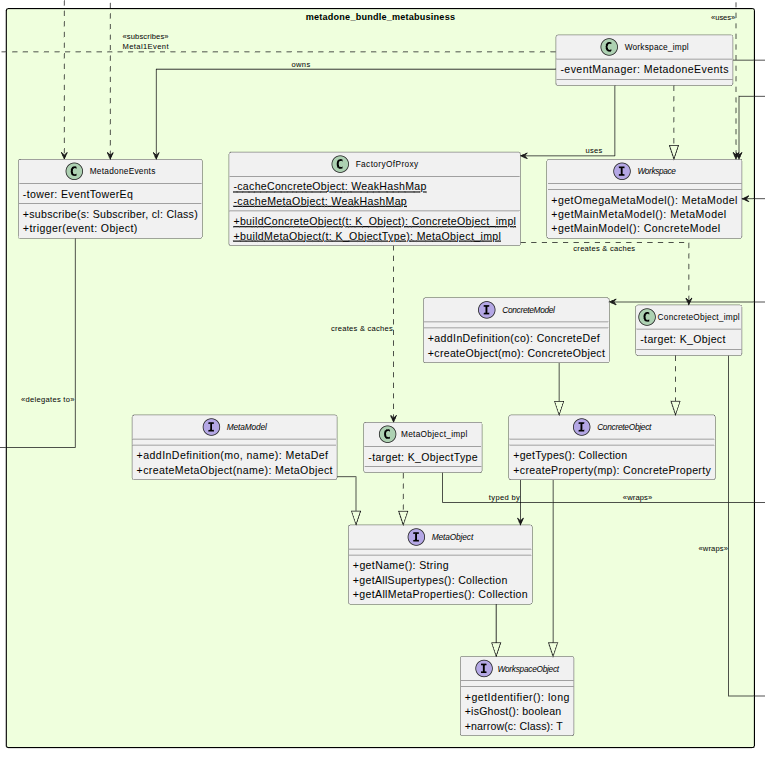
\includegraphics[width=0.7\textwidth]{img/architecture/bundle-MB.png}
\caption{Bundle metabusiness}
\label{bundle-MB}
\end{figure}

\subsection{Le patron Proxy : des interfaces sur des \texttt{DataObject}}
\label{sec:proxy}
Le premier principe architectural de ce bundle est l'usage systématique du patron de conception \textit{Proxy}. Chaque entité manipulée à travers les interfaces de MetaL$_2$ n'est pas un objet autonome : c'est un proxy léger qui encapsule un DataObject du bundle repository. Que l'entité soit un MetaObject, un MetaRole, un ConcreteObject ou un ConcreteRole, elle repose en dernière analyse sur un DataObject de MetaL$_1$, dont elle interprète les facettes à travers une interface
de plus haut niveau.

La classe abstraite \texttt{WorkspaceObject\_impl} constitue la base commune de
tous ces proxies. Elle maintient une référence vers le \texttt{Workspace\_impl}
courant et fournit l'opération de conversion sécurisée \texttt{narrow(Class<T>)},
qui tente de transtyper le proxy vers une interface plus spécifique et lève une
\texttt{BadPreCondition} si le transtypage est invalide.

La classe \texttt{FactoryOfProxy} centralise la création et la mise en cache des
proxies. Elle maintient des \texttt{WeakHashMap} associant chaque K\_Object ou
K\_ObjectType du repository à son proxy correspondant, garantissant que le même
DataObject produit toujours le même objet proxy. Ce cache à références faibles
permet au ramasse-miettes de récupérer les proxies inutilisés sans intervention
explicite.

\subsection{Implémentation de la couche méta-modèle (M2/M3)}
\label{sec:impl-metamodel}

La couche méta-modèle de MetaL$_2$ --- niveaux M2 et M3 de MetaL --- définit
les metaclasses qui permettent de décrire des domaines. Conformément à la
spécification formelle~\cite{englebert_metal2}, MetaObject, MetaRole, MetaProperty
et MetaModel héritent tous de MetaObject (sauf MetaObject lui-même), et MetaRole
est à la fois un type d'objet et un type de propriété.

La distinction clé avec la couche concrète réside dans la couche de MetaL$_1$
mobilisée : la couche méta-modèle s'appuie sur les \textbf{types} de MetaL$_1$
(K\_ObjectType, K\_PropertyType), là où la couche concrète s'appuie sur les
\textbf{instances} (K\_Object, K\_Property)~\cite{englebert_metal1}.

Dans l'implémentation, chaque concept correspond à une classe \texttt{*\_impl}
wrappant une facette de type du DataObject sous-jacent :

\begin{itemize}
  \item \texttt{MetaObject\_impl} encapsule un K\_ObjectType : un méta-objet est
    un type d'objet au sens du kernel, capable d'avoir des instances (K\_Object).
  \item \texttt{MetaRole\_impl} encapsule un K\_PropertyType : un méta-rôle est
    un type de propriété binaire orientée entre deux K\_ObjectType.
  \item \texttt{MetaProperty\_impl} encapsule également un K\_PropertyType
    spécialisé pour les attributs.
  \item \texttt{MetaDef\_impl} encapsule un K\_Property reliant un K\_ObjectType
    (l'objet membre, en position de domaine) à un K\_Object (le modèle, en position
    de range) ; il matérialise la relation \textit{PartWhole} de la spécification
    formelle~\cite{englebert_metal2}.
\end{itemize}

\texttt{MetaModel\_impl} étend \texttt{MetaObject\_impl} : un méta-modèle est
lui-même un méta-objet. Au niveau du kernel, il est représenté par un K\_ObjectType
avec la sémantique supplémentaire de conteneur de méta-objets.

\subsection{Le méta-méta-modèle Omega}

Un aspect fondamental de MetaL est que le niveau M3 est \textbf{réflexif} : les
metaclasses (MetaObject, MetaModel, MetaRole, MetaProperty) sont des instances
d'elles-mêmes~\cite{englebert_metal2}. Contrairement au MOF où M3 est
simplement \og conforme à lui-même \fg{}, MetaL en fait une \og vraie instance de
lui-même \fg{} --- une propriété formalisée dans~\cite{englebert_metal2}.

Le méta-modèle Omega, accessible via \texttt{Workspace.getOmegaMetaModel()},
matérialise ce niveau M3 dans MetaDONE. Il contient, en tant que MetaObject
ordinaires, les types primitifs du framework (String, Integer, Float, Boolean,
Char) ainsi que les metaclasses du framework elles-mêmes~: chacune est instance
d'elle-même --- \texttt{MetaObject} est instance de \texttt{MetaObject},
\texttt{MetaRole} est instance de \texttt{MetaRole}, \texttt{MetaProperty} est
instance de \texttt{MetaProperty}, et \texttt{MetaModel} est instance de
\texttt{MetaModel}.

Le méta-modèle principal de l'utilisateur, accessible via
\texttt{getMainMetaModel()}, est une instance de MetaModel (défini dans Omega) :
c'est le niveau M2. Les modèles concrets qui en sont instances constituent le
niveau M1.

\subsection{Implémentation de la couche concrète (M1)}
\label{sec:impl-concret}

Comme rappelé en section~\ref{sec:metal1}, MetaL$_1$ se limite au \texttt{DataObject}
et à ses facettes : aucun des concepts \texttt{ConcreteObject}, \texttt{ConcreteRole},
\texttt{ConcreteProperty} ou \texttt{ConcreteModel} n'appartient à cette couche. Tous
relèvent de MetaL$_2$~\cite{englebert_metal2}, au même titre que \texttt{MetaObject},
\texttt{MetaRole}, \texttt{MetaProperty} et \texttt{MetaModel}. La distinction interne à
MetaL$_2$ entre couche méta-modèle et couche concrète se traduit dans le choix des facettes
de MetaL$_1$ sur lesquelles elle s'appuie : la couche méta-modèle utilise les facettes de
\textbf{type} (\texttt{K\_ObjectType}, \texttt{K\_PropertyType}), la couche concrète celles
d'\textbf{instance} (\texttt{K\_Object}, \texttt{K\_Property})~\cite{englebert_metal1}.

Chaque concept de la couche concrète correspond à une classe \texttt{*\_impl} encapsulant
la facette appropriée :

\begin{itemize}
  \item \texttt{ConcreteObject\_impl} encapsule un K\_Object : un objet concret
    est une instance de K\_Object dont les types --- via la relation \textit{typeo}
    de MetaL$_1$ --- sont les K\_ObjectType correspondant aux MetaObject du
    méta-modèle.
  \item \texttt{ConcreteRole\_impl} encapsule un K\_Property et matérialise un
    lien concret entre deux ConcreteObject, instance d'un MetaRole.
  \item \texttt{ConcreteProperty\_impl} encapsule un K\_Property spécialisé
    portant une valeur primitive.
  \item \texttt{ConcreteDef\_impl} encapsule un K\_Property reliant un K\_Object
    (l'objet concret) à un K\_Object (le modèle), matérialisant la relation
    \textit{PartWhole} au niveau M1.
\end{itemize}

La réflexivité de MetaL$_2$ s'étend au niveau M1 : \texttt{ConcreteModel\_impl}
étend \texttt{ConcreteObject\_impl}, de sorte qu'un modèle concret est lui-même
un objet concret~\cite{englebert_metal2}. Il peut donc avoir des types,
des propriétés et participer à des rôles au même titre que n'importe quel élément
du modèle. C'est précisément cette uniformité qui permet à MetaDONE de stocker
ses scripts GraSyLa --- eux-mêmes des ConcreteObject --- dans le modèle et de les
manipuler avec les mêmes APIs que n'importe quel modèle utilisateur.

\section{Bundle \texttt{metadone\_bundle\_repository}}
\label{sec:repository}

Le bundle \texttt{metadone\_bundle\_repository} constitue la couche de persistance de MetaDONE (figure~\ref{bundle-repo}). Il définit un modèle de stockage minimaliste et générique --- le \emph{kernel} --- sur lequel reposent toutes les abstractions de MetaL$_1$ et MetaL$_2$ décrites précédemment. Ce bundle est purement abstrait : il ne contient que des interfaces et une classe abstraite, sans aucune dépendance vers une technologie de persistance concrète. Deux implémentations interchangeables en sont dérivées, présentées en fin de section.

\begin{figure}[h]
\centering
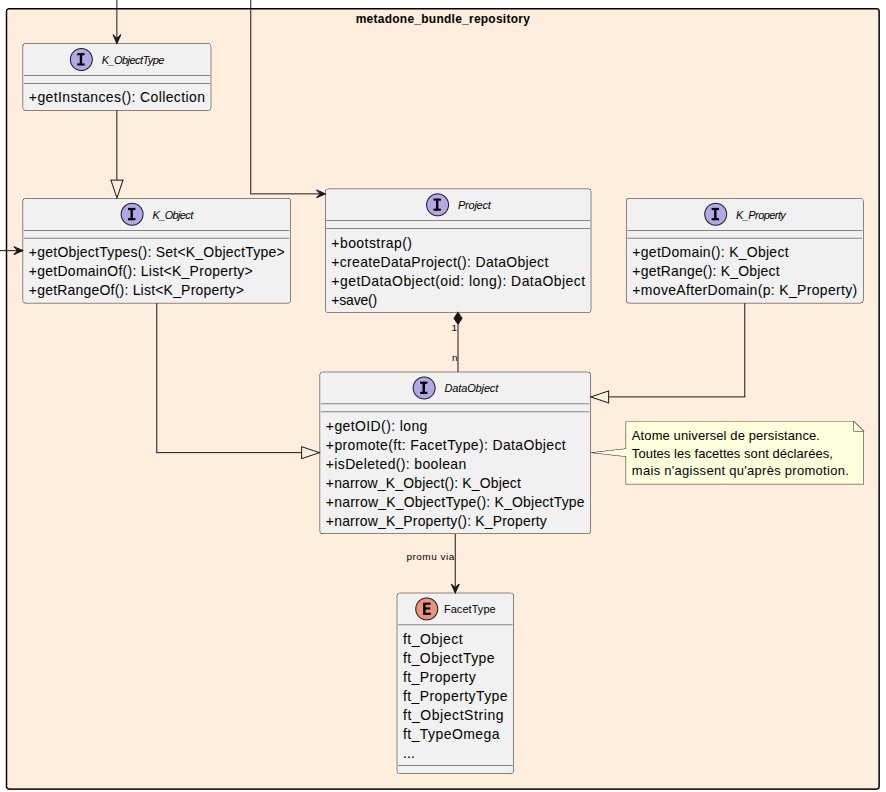
\includegraphics[width=0.7\textwidth]{img/architecture/bundle-repo.png}
\caption{Bundle repository}
\label{bundle-repo}
\end{figure}

\subsection{L'unité atomique : le \texttt{DataObject}}

Le \texttt{DataObject} est l'entité fondamentale du kernel. Chaque
élément du modèle, qu'il soit \texttt{MetaObject}, \texttt{MetaRole},
\texttt{ConcreteObject} ou \texttt{ConcreteProperty}, est en dernière analyse un \texttt{DataObject} persisté. Comme montré en
section~\ref{sec:impl-metamodel}, les classes \texttt{*\_impl} du bundle
métier sont toutes des proxies encapsulant un \texttt{DataObject}.

L'interface \texttt{DataObject} est remarquablement large : elle étend
simultanément l'ensemble des interfaces de facettes du kernel
(\texttt{K\_Common}, \texttt{K\_Object}, \texttt{K\_ObjectType},
\texttt{K\_Property}, \texttt{K\_PropertyType}, \texttt{K\_ObjectString},
\texttt{K\_ObjectInteger}, etc.), soit une quinzaine d'interfaces. Un
\texttt{DataObject} possède donc potentiellement toutes les capacités du
kernel, mais celles-ci ne sont activées qu'à la demande, via le mécanisme
de promotion.

\subsection{Le modèle de facettes et la promotion}

La flexibilité du kernel repose sur le concept de \emph{facette}. Plutôt
que de créer des types d'objets distincts pour chaque rôle possible, un
\texttt{DataObject} commence avec un ensemble vide de facettes actives et
se voit progressivement \emph{promu} vers de nouvelles capacités par
l'appel à \texttt{promote(FacetType)}. Cette promotion est irréversible
et cumulative : un objet peut acquérir plusieurs facettes compatibles.

L'enum \texttt{FacetType} liste les dix-sept facettes disponibles
(tableau~\ref{tab:facettypes}) et définit pour chacune sa
\emph{fermeture}, c'est-à-dire l'ensemble des facettes préalablement
requises. Par exemple, la promotion vers
\texttt{ft\_ObjectType} requiert \texttt{ft\_Common} et \texttt{ft\_Object},
et la promotion vers \texttt{ft\_PropertyTypePi} requiert \texttt{ft\_Common},
\texttt{ft\_Property} et \texttt{ft\_PropertyType}. Cette hiérarchie de
dépendances garantit la cohérence du modèle kernel.

\begin{table}[h]
\centering
\begin{tabular}{ll}
\hline
\textbf{Facette} & \textbf{Sémantique} \\
\hline
\texttt{ft\_Common} & Base commune à tout DataObject \\
\texttt{ft\_Object} & Objet pouvant avoir des types et des rôles \\
\texttt{ft\_ObjectType} & Type pouvant avoir des instances \\
\texttt{ft\_Property} & Lien orienté entre deux objets \\
\texttt{ft\_PropertyType} & Type de lien \\
\texttt{ft\_PropertyTypePi} & Type de lien racine (singleton) \\
\texttt{ft\_ObjectString/Integer/Float/Boolean/Char} & Valeur primitive \\
\texttt{ft\_TypeString/Integer/Float/Boolean/Char/Omega} & Type primitif prédéfini \\
\hline
\end{tabular}
\caption{Principales facettes du kernel MetaDONE}
\label{tab:facettypes}
\end{table}

\subsection{La hiérarchie des interfaces \texttt{K\_*}}

Chaque facette correspond à une interface \texttt{K\_*} qui expose les
opérations associées :

\begin{itemize}
    \item \texttt{K\_Object} : accès aux types de l'objet
    (\texttt{getObjectTypes()}), aux propriétés dont il est domaine
    (\texttt{getDomainOf()}) ou codomaine (\texttt{getRangeOf()}).
    \item \texttt{K\_ObjectType} : accès aux instances du type
    (\texttt{getInstances()}) et navigation dans la hiérarchie de
    sous-types.
    \item \texttt{K\_Property} : accès au domaine (\texttt{getDomain()})
    et au codomaine (\texttt{getRange()}) du lien, gestion de l'ordre
    dans les listes (\texttt{moveAfterDomain()},
    \texttt{moveLastRange()}).
    \item \texttt{K\_PropertyType} : type d'un lien, associant un type
    de domaine et un type de codomaine.
    \item \texttt{K\_ObjectString}, \texttt{K\_ObjectInteger}, etc. :
    stockage d'une valeur primitive du type correspondant.
\end{itemize}

Le transtypage vers une interface précise s'effectue via les méthodes
\texttt{narrow\_K\_*()} du \texttt{DataObject}, qui retournent
\texttt{null} si la facette requise n'est pas active. L'invocation
ultérieure d'une opération sur une facette inactive (par exemple
\texttt{getDomain()} sur un DataObject sans facette \texttt{Property})
lève alors une \texttt{BadFacet}.

\subsection{Les relations de typage et de sous-typage}

Deux relations N-N fondamentales structurent le kernel.
\texttt{NN\_typeof} matérialise le lien \emph{instance-de} entre un
\texttt{K\_Object} et un \texttt{K\_ObjectType} : c'est par cette
relation qu'un \texttt{ConcreteObject} est lié à son
\texttt{MetaObject}. \texttt{NN\_subtype} matérialise le lien
\emph{sous-type-de} entre deux \texttt{K\_ObjectType} : c'est par cette
relation que l'héritage entre \texttt{MetaObject} est persisté.

Ces relations sont des objets explicites, ce qui permet de les naviguer dans les deux sens et de les
gérer via le cycle de vie standard (\texttt{PersistenceLifeCycle}).

\subsection{Le \texttt{Project} et le bootstrap}

Le \texttt{Project} est le conteneur racine de tous les
\texttt{DataObject}. Il joue deux rôles : celui de factory
(\texttt{FactoryData}) pour la création des entités, et celui de registre
des types primitifs prédéfinis. L'opération \texttt{bootstrap()} est
appelée à l'initialisation du projet et crée les singletons de types
primitifs (\texttt{K\_TypeInteger}, \texttt{K\_TypeString},
\texttt{K\_TypeFloat}, \texttt{K\_TypeBoolean}, \texttt{K\_TypeChar} et
\texttt{K\_TypeOmega}) ainsi que le type racine de toutes les propriétés \texttt{K\_PropertyTypePi}.

La classe abstraite \texttt{AbstractProject} fournit l'infrastructure
événementielle du kernel. Elle maintient un \texttt{EventTower<Metal1Event>}
et déclenche des événements de bas niveau à chaque modification
structurelle : \texttt{EventCreateDataObject} à la création,
\texttt{EventLink} au lien de sous-typage ou de typage,
\texttt{EventWillDelete} avant suppression, \texttt{EventChange} et
\texttt{EventChangeFacet} lors de modifications. Ces événements sont
capturés par \texttt{Workspace\_impl} pour être traduits en événements
MetaL$_2$ plus riches.

\subsection{Implémentation JPA2 :
\texttt{metadone\_bundle\_repository\_jpa2}}

Le bundle \texttt{metadone\_bundle\_repository\_jpa2} fournit une
implémentation relationnelle du kernel, reposant sur
\emph{Apache OpenJPA 2.3.0}. La classe \texttt{DataObjectJPA2} est
annotée \texttt{@Entity} et mappée vers une table relationnelle unique par
un schéma de type \emph{single-table inheritance}.

La sérialisation de l'ensemble de facettes actives d'un
\texttt{DataObject} est réalisée via la classe \texttt{Facets}, qui
encode un \texttt{EnumSet<FacetType>} en un entier par manipulation de
bits (\texttt{jpaExtern}) et le reconstitue à la lecture
(\texttt{jpaBuild}). Ce choix de représentation compacte réduit
l'empreinte mémoire et le coût d'accès en base.

Les relations N-N (\texttt{NN\_typeofJPA2}, \texttt{NN\_subtypeJPA2})
sont mappées avec des annotations \texttt{@OneToMany} et
\texttt{@ManyToOne}. Les requêtes nécessitant un filtrage sur les types
ou les sous-types utilisent l'API JPA Criteria, évitant la construction
de JPQL sous forme de chaînes de caractères. La classe
\texttt{ProjectJPA2} gère la transaction via un \texttt{EntityManager}
JPA standard, encapsulé dans \texttt{TransactionJPA2}.

\subsection{Implémentation ObjectDB :
\texttt{metadone\_bundle\_repository\_odb}}

Le bundle \texttt{metadone\_bundle\_repository\_odb} fournit une
implémentation alternative reposant sur \emph{ObjectDB 2.5.7}, une base
de données orientée objet pour Java, compatible JPA. La classe
\texttt{DataObjectODB} utilise les mêmes annotations JPA que son
homologue JPA2 (\texttt{@Entity}, \texttt{@Id}, \texttt{@OneToMany},
etc.), ObjectDB implémentant nativement la spécification JPA sans couche
ORM intermédiaire.

L'intérêt de cette implémentation réside dans l'alignement naturel entre
le modèle objet Java et le moteur de stockage : les objets sont persistés
tels quels, sans transformation relationnelle. Cela simplifie les
stratégies de mapping et peut réduire l'impedance objet-relationnel
présente dans l'implémentation JPA2. La transaction est gérée par
\texttt{TransactionODB}, qui encapsule le mécanisme de transaction propre
à ObjectDB.

\subsection{Substitution par OSGi}

Les deux implémentations exposent un service \texttt{FactoryProject} dans
le registre OSGi via leur \texttt{Activator} respectif. Le bundle
\texttt{metadone\_bundle\_metabusiness} découvre ce service à travers son
\texttt{RepositoryTracker} : selon le bundle repository démarré par
Equinox, l'implémentation JPA2 ou ODB est sélectionnée de manière transparente,
sans que le reste de l'application n'en soit informé. Ce mécanisme
illustre concrètement le bénéfice de l'architecture OSGi pour
l'interchangeabilité des composants à l'exécution.

\section{Bundle \texttt{metadone\_common}}

Le bundle \texttt{metadone\_common} est une bibliothèque d'infrastructure
partagée par l'ensemble des bundles de MetaDONE (figure~\ref{bundle-common}). Il ne contient aucune
logique métier, mais fournit les abstractions transversales sur lesquelles
repose toute l'architecture : système de notification, utilitaires de
collections et hiérarchie d'exceptions.

\begin{figure}[h]
\centering
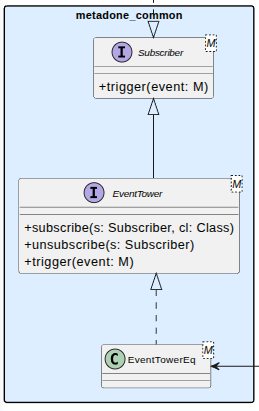
\includegraphics[width=0.3\textwidth]{img/architecture/bundle-common.png}
\caption{Bundle common}
\label{bundle-common}
\end{figure}

\subsection{Le système publish-subscribe}

Le sous-package \texttt{publish\_subscribe} définit le mécanisme de
notification réactif utilisé à travers tous les niveaux de
l'architecture : \texttt{AbstractProject} l'utilise pour les événements
kernel (\texttt{Metal1Event}), \texttt{MetadoneEvents} l'utilise pour les
événements métier (\texttt{Metal2Event}), et les engines GraSyLa
s'abonnent aux changements du workspace pour se rafraîchir
automatiquement.

Le contrat central est l'interface \texttt{EventTower<M>}, qui étend
elle-même \texttt{Subscriber<M>} : une tour d'événements est donc aussi
un souscripteur, ce qui permet de composer et chaîner des tours.
L'abonnement est filtré à deux niveaux : par \emph{type Java} de
l'événement (via \texttt{Class<T>}) et, optionnellement, par
\emph{prédicat} (\texttt{MapFct<T, Boolean>}).

Trois implémentations de \texttt{EventTower} sont proposées :
\begin{itemize}
    \item \texttt{EventTowerNormal} : implémentation de base maintenant
    une liste de nœuds d'abonnement indexés par classe d'événement.
    \item \texttt{EventTowerEq} : extension optimisée de
    \texttt{EventTowerNormal} qui reconnaît le motif de prédicat
    le plus fréquent dans MetaDONE --- tester l'égalité d'un attribut
    de l'événement à une valeur fixe (\texttt{MapFcts.Equal}) --- et
    les indexe dans une \texttt{HashMap} pour un dispatch en O(1) plutôt
    qu'une évaluation linéaire des prédicats. C'est cette implémentation
    qu'utilise \texttt{MetadoneEvents}.
    \item \texttt{EventTowerBuffer} : implémentation qui accumule les
    événements dans un tampon avant de les dispatcher, utile pour
    grouper des modifications en rafale.
\end{itemize}

La classe \texttt{AbstractSubscription} encapsule le cycle de vie d'un
abonnement (souscription et désabonnement) et sert de base à
\texttt{Subscription} (abonnement simple) et
\texttt{SubscriberHandler} (abonnement avec délégation à un
\texttt{Consumer} fonctionnel).

\subsection{Utilitaires}

Le sous-package \texttt{util} regroupe des structures de données et des
fonctions utilitaires employées intensivement dans les couches
supérieures.

Parmi les structures notables dans le contexte de l'optimisation,
\texttt{CacheCallFunction<Arg, Ret>} est une structure de mémoïsation
générique : elle associe une valeur de retour à chaque argument
d'appel dans une \texttt{HashMap} et peut être désactivée par
configuration pour désactiver le cache sans modifier le code appelant.
\texttt{LazySet<E>} est un proxy copy-on-write sur un \texttt{Set} : il
référence le set original sans le copier tant qu'aucune modification
n'est effectuée, ce qui réduit l'allocation mémoire dans les scénarios
de lecture dominante.

Les autres utilitaires couvrent les besoins courants : \texttt{Pair<A,B>}
et \texttt{BiDir<A,B>} pour les associations bidirectionnelles,
\texttt{MapFct<A,B>} comme interface fonctionnelle précédant les lambdas
Java 8, \texttt{ImmutableList}, \texttt{ListUtil}, \texttt{SetUtil} et
\texttt{IteratorUtil} pour la manipulation de collections, et
\texttt{Chrono} pour la mesure des temps d'exécution.

\subsection{Exceptions}

La hiérarchie d'exceptions maison couvre les cas les plus fréquents :
\texttt{BadPreCondition} (et sa spécialisation \texttt{NullArgument})
pour les violations de contrats d'entrée, \texttt{InternalException}
pour les erreurs internes inattendues, \texttt{FailedOperation} pour les
opérations échouées de façon récupérable, et \texttt{NotYetImplemented}
comme marqueur de code à compléter.

\section[Synthèse]{Synthèse : réflexivité et omniprésence des \texttt{DataObject}}
\label{sec:reflexivite}

Les quatre bundles présentés dans ce chapitre forment un système cohérent
dont deux propriétés architecturales transversales méritent d'être mises
en lumière avant d'aborder l'optimisation : la \emph{réflexivité} du
modèle à niveaux, et l'\emph{omniprésence} du \texttt{DataObject} comme substrat universel de persistance.

\subsection{Une architecture réflexive}

La réflexivité de MetaDONE signifie que le framework se décrit lui-même
avec ses propres outils. Cette propriété se manifeste à plusieurs niveaux.

Au niveau de MetaL$_2$, \texttt{MetaModel} étend \texttt{MetaObject} : un
méta-modèle est lui-même un méta-objet, susceptible d'avoir des types,
des propriétés et des rôles. Le méta-modèle Omega, accessible via
\texttt{Workspace.getOmegaMetaModel()}, contient en tant que
\texttt{MetaObject} ordinaires les concepts de MetaL$_2$ lui-même ainsi que les types primitifs. MetaDONE utilise
donc ses propres APIs pour naviguer dans sa propre structure.

Au niveau de MetaL$_1$, \texttt{ConcreteModel} étend \texttt{ConcreteObject}
: un modèle concret est lui-même un objet concret, instance d'un
\texttt{MetaModel}. La hiérarchie est ainsi uniforme et récursive à
chaque niveau.

La conséquence la plus frappante de cette réflexivité est que les scripts
GraSyLa (le langage de description de vues présenté en
section~\ref{sec:grasyla}) sont eux-mêmes stockés dans le modèle MetaDONE sous forme de \texttt{ConcreteObject}. Une équation GraSyLa est une instance d'un \texttt{MetaObject} défini dans le méta-modèle Omega ;
ses membres gauche et droit sont accessibles et modifiables via les APIs
standard de MetaL$_1$. Le moteur de rendu, le langage de vue et les données
métier partagent ainsi le même substrat de représentation, sans
distinction de nature.

Cette uniformité est un atout de conception : elle permet de manipuler
n'importe quel aspect du système --- modèle, méta-modèle, scripts de
visualisation, configuration --- avec un seul ensemble d'APIs. Elle a
néanmoins une contrepartie directe sur les performances, que nous allons
à présent examiner.

\subsection{L'omniprésence du \texttt{DataObject}}

Le patron Proxy présenté en section~\ref{sec:impl-metamodel} a une
implication quantitative forte : en pratique, la quasi-totalité des
entités manipulées par MetaDONE sont des \texttt{DataObject} du kernel,
enveloppés dans des proxies sémantiques.

\begin{itemize}
    \item Chaque \texttt{MetaObject} est un proxy sur un
    \texttt{K\_ObjectType}, lui-même un \texttt{DataObject} promu
    \texttt{ft\_ObjectType}.
    \item Chaque \texttt{MetaRole} et \texttt{MetaProperty} sont des
    proxies sur un \texttt{K\_PropertyType}, soit un \texttt{DataObject}
    promu \texttt{ft\_PropertyType}.
    \item Chaque \texttt{ConcreteObject} est un proxy sur un
    \texttt{K\_Object}, soit un \texttt{DataObject} promu
    \texttt{ft\_Object}.
    \item Chaque \texttt{ConcreteRole} et \texttt{ConcreteProperty} sont
    des proxies sur un \texttt{K\_Property}, soit un \texttt{DataObject}
    promu \texttt{ft\_Property}.
    \item Chaque \texttt{MetaDef} et \texttt{ConcreteDef} sont des
    proxies sur un \texttt{K\_Property} reliant deux \texttt{DataObject}.
    \item Chaque nœud de l'arbre d'expression d'une équation GraSyLa est
    un \texttt{ConcreteObject}, donc lui aussi un \texttt{DataObject}.
\end{itemize}

Les seules entités qui ne sont pas directement des \texttt{DataObject}
sont les liaisons de typage (\texttt{NN\_typeof}) et de sous-typage
(\texttt{NN\_subtype}), qui sont des enregistrements de relation distincts mais qui sont eux-mêmes persistés et gérés par le kernel.

Il résulte de cette conception que l'ensemble du contenu d'un projet MetaDONE est représenté par un graphe homogène de \texttt{DataObject} liés entre
eux par des \texttt{K\_Property} (relations) et des
\texttt{NN\_typeof}/\texttt{NN\_subtype} (typage et héritage).

\subsection{Des algorithmes complexes sur un substrat homogène}

L'homogénéité du substrat, si elle simplifie la conception, engendre une
classe de problèmes de performance caractéristiques. Puisque toute
sémantique est encodée dans le graphe de \texttt{DataObject}, les
opérations logiquement simples requièrent des traversées récursives de ce
graphe.

L'opération \texttt{getMOByName}, par exemple, doit naviguer
récursivement dans l'arbre des \texttt{MetaModel} en traversant les
\texttt{K\_Property} de définition, puis filtrer les \texttt{MetaObject}
par nom --- une recherche linéaire sur des \texttt{DataObject}. Dans les
modèles de taille réelle, cette opération est appelée de manière répétée
lors du bootstrap, de l'import et du rendu GraSyLa.

L'opération \texttt{\_isInDefinition}, appelée à chaque ajout d'un
\texttt{ConcreteObject} dans un \texttt{ConcreteModel}, doit parcourir
l'ensemble des propriétés du modèle pour vérifier qu'un objet n'y est
pas déjà présent. Sans précaution, chaque appel à
\texttt{addInDefinition} déclenche un scan linéaire de l'ensemble de la
définition du modèle.

De même, les algorithmes de navigation des hiérarchies de types ---
\texttt{getAllSupertypes()}, \texttt{getAllSubtypes()},
\texttt{getAllMetaProperties()} --- doivent traverser les chaînes
\texttt{NN\_subtype} de manière récursive, ce qui dans une hiérarchie
profonde engendre un nombre d'accès aux \texttt{DataObject} croissant
avec la profondeur de l'arbre.

\subsection{Les optimisations comme réponse structurelle}

Les travaux d'optimisation conduits dans le cadre de ce mémoire
s'inscrivent directement dans ce contexte. Les principales interventions
portent sur la mise en cache stratégique des résultats de ces traversées
coûteuses.

Dans \texttt{ConcreteModel\_impl}, un cache de type
\texttt{WeakHashMap<ConcreteObject\_impl, Boolean>} mémorise les
résultats de \texttt{\_isInDefinition} : la vérification d'appartenance
passe ainsi d'un scan linéaire à un accès en O(1) pour les appels
ultérieurs. Ce cache est mis à jour de façon incrémentale lors de
\texttt{addInDefinition} --- sans nécessiter de re-scan --- et invalidé
lors de \texttt{removeFromDefinition}.

Dans \texttt{MetaModel\_impl}, la \texttt{CacheCallFunction} du bundle
\texttt{metadone\_common} est utilisée pour mémoïser les résultats de
\texttt{getMetaObjectsInDefinition}, indexés par l'OID du
\texttt{DataObject} sous-jacent. Cette clé d'indexation par OID est
précisément rendue possible par l'omniprésence des \texttt{DataObject} :
chaque entité possède un identifiant stable et unique dans le kernel,
directement accessible depuis le proxy.

L'usage de \texttt{WeakHashMap} dans les deux cas garantit que les
entrées de cache sont récupérées par le ramasse-miettes dès que le proxy
correspondant n'est plus référencé, évitant toute fuite mémoire dans un
système où les objets peuvent être supprimés à l'exécution.

Ces optimisations illustrent une tension fondamentale inhérente à l'architecture réflexive de MetaDONE : la généricité et l'uniformité du substrat \texttt{DataObject} sont des atouts de conception, mais transfèrent la complexité vers les algorithmes qui doivent interpréter et naviguer ce graphe homogène. Le chapitre suivant présente une analyse systématique de ces goulots d'étranglement et les stratégies mises en œuvre pour les résoudre.

\chapter{Méthodologie}
\label{chap:methodologie}

L'optimisation de MetaDONE s'inscrit dans une démarche structurée qui part des usages réels du logiciel, identifie empiriquement les goulots d'étranglement, et évalue rigoureusement l'impact de chaque intervention. Cette section présente les fondements méthodologiques de notre approche.

% - - - - - - - - - - -
\section{Approche par scénarios représentatifs}
% - - - - - - - - - - -

Toute démarche d'optimisation sérieuse doit reposer sur des mesures plutôt que sur des intuitions. La règle empirique bien établie, attribuée à Donald Knuth, est que la grande majorité du temps d'exécution d'un programme est concentrée dans une fraction minoritaire du code~\cite{knuth1974structured}. Optimiser une méthode rarement exécutée n'a aucun impact mesurable~; à l'inverse, réduire de moitié le coût d'une méthode appelée des millions de fois peut transformer l'expérience utilisateur.

Dans ce mémoire, nous adoptons une approche par \textbf{scénarios représentatifs}~: plutôt que d'analyser le code en chambre, nous définissons un ensemble de cas d'utilisation typiques qui capturent les interactions les plus fréquentes ou les plus coûteuses avec MetaDONE. Cette approche est cohérente avec les recommandations de la littérature sur l'optimisation de logiciels complexes~\cite{oaks2014java, arcelli2018performance}, qui soulignent l'importance d'ancrer les mesures dans des \textit{workloads} représentatifs
plutôt que dans des microbenchmarks artificiels.

Les scénarios retenus sont définis et justifiés à la
section~\ref{sec:scenarios}.

% - - - - - - - - - - -
\section{Le cycle mesure–analyse–optimisation}
\label{sec:cycle}
% - - - - - - - - - - -

Notre démarche s'articule autour d'un cycle itératif en quatre phases,
synthétisé dans la figure~\ref{fig:opti-cycle}.
\begin{enumerate}
    \item \textbf{Préparation.} Définition du scénario, mise en place des
    outils de mesure, et établissement d'une ligne de base (\textit{baseline})
    --- c'est-à-dire une mesure de référence des performances avant toute
    modification. La baseline est indispensable pour quantifier objectivement
    les gains obtenus.

    \item \textbf{Identification des goulots d'étranglement.} Profilage de l'application sur le scénario cible afin de localiser les méthodes ou composants dominant le temps d'exécution~\cite{knuth1974structured,oaks2014java}. 

    \item \textbf{Optimisation.} Implémentation d'une correction ciblée sur
    le goulot identifié. Une seule modification à la fois est préférable afin de pouvoir attribuer causalement tout gain ou régression observés~\cite{oaks2014java}.

    \item \textbf{Tests de performance.} Exécution du scénario après
    modification et comparaison avec la baseline. Si le gain est insuffisant
    ou si un nouveau goulot apparaît, le cycle reprend à l'étape
    d'identification.
\end{enumerate}

\begin{figure}[h]
    \centering
    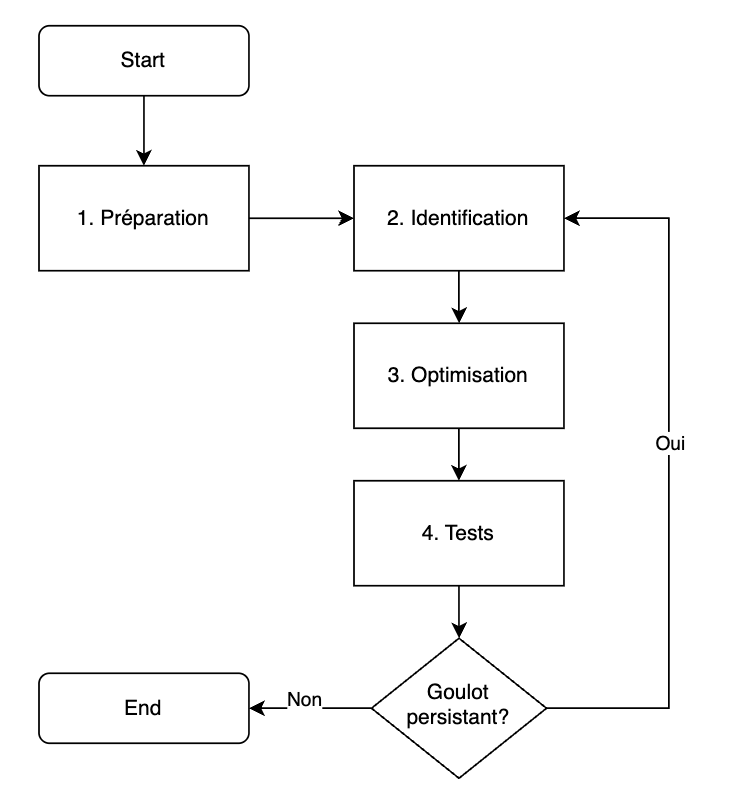
\includegraphics[width=0.5\textwidth]{img/mesure-analyse-opti.png}
    \caption{Cycle itératif mesure--analyse--optimisation.}
    \label{fig:opti-cycle}
\end{figure}

% - - - - - - - - - - -
\section{Environnement expérimental et outils de mesure}
\label{sec:env}
% - - - - - - - - - - -

\paragraph{Configuration matérielle et logicielle.}
Les expériences ont été réalisées sur une machine équipée d'un processeur AMD
Ryzen 5 9600X (6 cœurs, 12 threads, 65W TDP), disposant de 32~Go de mémoire
vive DDR5 cadencée à 6000~MHz et d'un stockage SSD NVMe. Ce choix matériel
vise à minimiser l'impact des I/O disque et de la latence mémoire sur les
mesures, de sorte que les goulots observés reflètent le comportement applicatif
plutôt que les limitations de l'infrastructure.

Le système d'exploitation est Linux (architecture x86\_64). L'environnement
d'exécution est Java 8 (JDK 1.8), qui correspond à la version cible de
MetaDONE déployée dans Eclipse Oxygen (4.7.0). Ce choix contraint certaines
options de collecteur GC disponibles dans les versions ultérieures du JDK
(ZGC et Shenandoah n'étant disponibles qu'à partir de Java 11 et 12
respectivement), mais garantit la fidélité des résultats à l'environnement
de production réel de l'outil.

\paragraph{Reproductibilité des mesures.}
Chaque scénario a été exécuté 10 fois et les résultats présentés correspondent aux valeurs médianes des 10 mesures. La médiane est préférée à la moyenne car elle est plus robuste aux valeurs aberrantes liées aux pauses du \textit{Garbage Collector} ou aux interruptions du système d'exploitation~\cite{georges2007statistically}~: avec 10 répétitions, elle absorbe jusqu'à 4 valeurs aberrantes sans biais. Pour chaque scénario, le \textbf{coefficient de variation} (CV~$= \sigma / \mu$) a également été calculé afin de vérifier la stabilité des mesures~: un CV faible (typiquement inférieur à 5\,\%) confirme que 10 répétitions sont suffisantes pour obtenir une médiane stable. Aucune phase de warmup de la JVM n'a en revanche été instaurée, faute de temps~; cette limite est discutée au chapitre~\ref{chap:discussion}, où l'on s'assure que les ordres de grandeur des gains observés en sont peu affectés.

\paragraph{Outils de profilage.}
Deux outils complémentaires ont été retenus, dont le choix est justifié dans
le tableau~\ref{tab:profilers}.

\begin{table}[h]
\centering
\caption{Comparaison des principaux outils de profilage Java}
\label{tab:profilers}
\small
\begin{tabular}{lllll}
\hline
\textbf{Outil} & \textbf{Méthode} & \textbf{Surcoût} &
\textbf{Domaine} & \textbf{Visualisation} \\
\hline
JVisualVM    & Sampling/instrum. & Moyen    & CPU, heap       & GUI intégrée \\
JFR + JMC    & Sampling faible   & Très faible & CPU, GC, I/O, locks & Flight Recorder \\
async-profiler & Perf events     & Quasi nul & CPU (wall/alloc) & Flamegraph SVG \\
JProfiler    & Instrumentation   & Élevé    & CPU, mémoire, JDBC & GUI riche \\
YourKit      & Sampling/instrum. & Moyen    & CPU, mémoire    & GUI riche \\
\hline
\end{tabular}
\end{table}

Parmi les cinq outils du tableau~\ref{tab:profilers}, seuls \textbf{JFR} et \textbf{async-profiler} ont été retenus. JVisualVM, JProfiler et YourKit ont été écartés en raison d'un surcoût d'instrumentation jugé incompatible avec des mesures représentatives à grande échelle.

\textbf{Java Flight Recorder (JFR)} est utilisé pour les mesures de
durée globale et l'analyse des événements GC, des locks et des accès I/O
sur l'ensemble d'un scénario. Son surcoût inférieur à 1\,\% en fait
l'outil de référence pour les mesures de longue durée sans biais
d'observation~\cite{jfr2021oracle}.

\textbf{async-profiler}~\cite{asyncprofiler} est utilisé pour localiser précisément les
méthodes chaudes (\textit{hotspots}) via des flamegraphs. Il s'appuie sur
les compteurs de performance matériels du CPU via \texttt{perf\_events}
plutôt que sur l'instrumentation JVM, ce qui élimine le biais du
\textit{safepoint sampling} qui affecte les profileurs JVM classiques~\cite{mytkowicz2010evaluating}. Les deux outils sont complémentaires~: JFR mesure \textit{quoi} et \textit{combien}, async-profiler localise \textit{où}.

\section[Scénarios représentatifs]{Scénarios représentatifs des usages de MetaDONE}
\label{sec:scenarios}

La sélection des scénarios suit trois critères~: la \textbf{fréquence} (les
opérations exécutées à chaque session de travail), la \textbf{criticité}
(les opérations dont la latence est directement perçue par l'utilisateur)
et la \textbf{scalabilité} (les opérations dont le coût croît avec la
taille du projet et qui révèlent d'éventuelles dégradations non-linéaires).
Les deux premiers critères sont cohérents avec la recommandation générale
de concentrer les efforts sur les chemins d'exécution à fort
impact~\cite{oaks2014java}~; le troisième complète cette démarche en
exposant les hypothèses architecturales à l'épreuve du volume.

Quatre scénarios ont finalement été retenus, couvrant des parties significatives du cycle de vie d'une session MetaDONE~\footnote{Un cinquième scénario, dédié à la modification et au rechargement itératif d'un script GraSyLa, avait initialement été planifié sous le numéro S3, mais a été écarté en cours de mémoire au profit d'une analyse plus approfondie de la boucle de visualisation (S4). La numérotation des scénarios suivants a été conservée pour rester cohérente avec les comptes-rendus intermédiaires.}~:

\begin{description}
    \item[Scénario~1~: Phase d'initialisation.] Au démarrage de MetaDONE, le dépôt est ouvert et les items séminaux de MetaL$_1$ ainsi que le métamétamodèle MetaL$_2$ sont chargés depuis la base de données. Cette phase est exécutée à chaque lancement et constitue le premier point de friction pour l'utilisateur. Elle implique la résolution des cycles de la relation \texttt{instanceOf} décrits à la section~\ref{sec:graphes-cycliques}, et constituera donc l'occasion de tester l'hypothèse formulée en section~\ref{sec:persistance-openjpa} selon laquelle ce chargement souffrirait du problème du N+1 et des limites du lazy loading.

    \item[Scénario~2~: Chargement d'un script GraSyLa.] L'ouverture d'un
    projet existant nécessite le chargement du script GraSyLa associé à son
    métamodèle, puis la construction de l'arbre d'expressions correspondant
    en mémoire. Ce scénario implique des traversées répétées du graphe
    méta-circulaire et est représentatif des sessions de modélisation
    quotidiennes.

    \item[Scénario~4~: Visualisation d'un (méta)modèle.] Le rendu graphique d'un modèle par GraSyLa implique l'évaluation de l'ensemble des équations du script pour chaque objet du modèle. Sur des modèles de taille significative, ce scénario met en évidence les coûts de traversée de graphe et d'évaluation des expressions.

    \item[Scénario~5~: Création et persistance d'un grand modèle (réseau de Petri).] Pour évaluer le comportement de MetaDONE à l'échelle, ce scénario construit programmatiquement un réseau de Petri de taille croissante, le visualise, puis le sauvegarde dans le dépôt. Il permet d'évaluer la scalabilité de la persistance JPA sur des volumes importants d'éléments de même type et de vérifier l'absence de dégradation non-linéaire des performances. Ce scénario relève moins de l'usage quotidien que des deux premiers et illustre le critère de scalabilité introduit ci-dessus.
\end{description}

Ces scénarios sont traités dans les sections suivantes selon le cycle itératif décrit à la section~\ref{sec:cycle}. Chaque section commence par une description de la baseline mesurée, puis alterne phases d'identification et d'optimisation jusqu'à convergence vers un résultat satisfaisant ou jusqu'à identification d'une limite structurelle de l'architecture actuelle.
\chapter{Développement}
\label{chap:developpement}
\section{Scénario 1 : Phase d'initialisation}
\label{sec:scenario1}

Le premier scénario ciblé est la \textbf{phase d'initialisation} de MetaDONE, c'est-à-dire la séquence complète qui s'étend de l'ouverture d'un projet jusqu'à l'état \texttt{PROJECT\_DEFAULT\_REPOSITORY IS OPENED}, tel qu'il apparaît dans les logs (figure~\ref{fig:logs-startup}). Cette phase est exécutée à chaque lancement de l'outil et constitue le premier point de friction perçu par l'utilisateur~: la médiane de nos mesures est de \textbf{18\,198~ms} (min~17\,673 / max~18\,650 ; CV~$=$~1,8\,\%), calculée sur 10 répétitions dans l'environnement décrit à la section~\ref{sec:env} (mesures complètes en annexe~\ref{ann:mesures-s1-a}).

\begin{figure}[h]
\centering
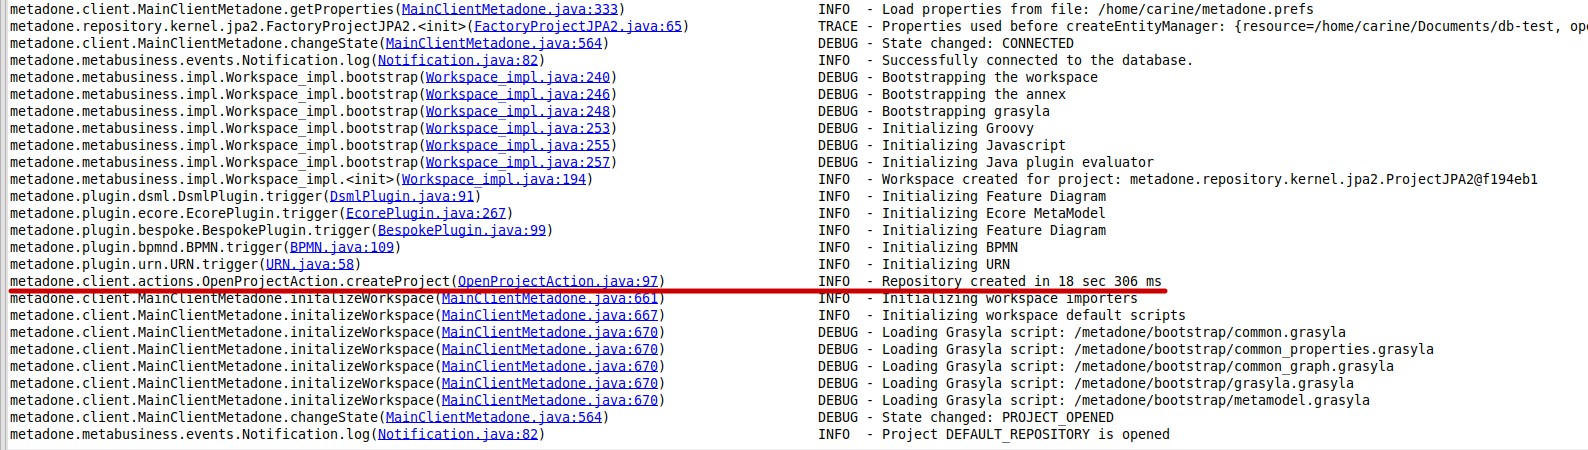
\includegraphics[width=\textwidth]{img/scenario1/ouverture-1.png}
\caption{Séquence de démarrage de MetaDONE. On distingue les trois phases de bootstrapping (\texttt{workspace}, \texttt{annex},
\texttt{grasyla}) ainsi que l'initialisation des plugins.}
\label{fig:logs-startup}
\end{figure}

Les logs révèlent une séquence structurée en plusieurs étapes distinctes, dont la compréhension est indispensable pour interpréter les résultats
de profilage.

La séquence débute par la connexion à la base de données (\texttt{FactoryProjectJPA2.<init>}) et l'initialisation du gestionnaire JPA (\texttt{createEntityManager}). Vient ensuite le \textbf{bootstrapping},
qui construit en mémoire le graphe réflexif de MetaL$_1$ et MetaL$_2$ à partir de zéro~: il crée les items séminaux (\texttt{Bootstrapping the workspace}), puis le méta-méta-modèle Omega et les types primitifs (\texttt{Bootstrapping the annex}), et enfin charge les scripts GraSyLa de base (\texttt{Bootstrapping grasyla}). Ces trois sous-phases opèrent dans \texttt{Workspace\_impl.bootstrap()} du bundle \texttt{metadone\_bundle\_metabusiness}.

Une fois le \texttt{Workspace} créé, les \textbf{plugins OSGi} sont déclenchés séquentiellement via leur méthode \texttt{trigger()}. Les logs montrent l'initialisation de \texttt{EcoreMetaModel}, \texttt{FeatureDiagram} (déclenché indépendamment par \texttt{DsmlPlugin} puis par \texttt{BespokePlugin}), \texttt{BPMN} et \texttt{URN}.

Enfin, le workspace charge les scripts GraSyLa applicatifs (\texttt{common.grasyla}, \texttt{common\_properties.grasyla}, etc.) via
\texttt{MainClientMetadone.initializeWorkspace()}, avant d'atteindre l'état
\texttt{PROJECT DEFAULT\_REPOSITORY IS OPENED}.

\subsection{Identification des goulots d'étranglement}
\label{sec:scenario1-profil1}

Cette phase d'analyse vise à isoler précisément les sections du code
responsables d'une consommation excessive de ressources. Comme présenté à
la section~\ref{sec:env}, JFR et async-profiler sont deux outils
complémentaires~: JFR fournit une vue structurée des événements JVM sur
l'ensemble de la durée de démarrage, tandis qu'async-profiler localise
précisément les méthodes dominantes via un échantillonnage non biaisé par
le mécanisme de safepoint~\cite{mytkowicz2010evaluating}.

% -----------------------------------------------
\subsubsection{Profilage avec Java Flight Recorder}
% -----------------------------------------------

L'activation de JFR au lancement de la JVM utilise les arguments suivants~:

\begin{verbatim}
-XX:+UnlockCommercialFeatures
-XX:+FlightRecorder
-XX:StartFlightRecording=name=metadone_jfr,settings=profile,
    dumponexit=true,filename=metadone.jfr
-XX:FlightRecorderOptions=stackdepth=256
\end{verbatim}

L'option \texttt{settings=profile} active le profil de collecte étendu,
qui enregistre davantage d'événements au prix d'un surcoût légèrement
supérieur au profil \texttt{default} (environ 2\% contre 1\% selon la
documentation Oracle~\cite{jfr2021oracle}). L'option \texttt{stackdepth=256} augmente la profondeur de pile enregistrée au-delà de la valeur par défaut de 64, ce qui est nécessaire ici~: l'architecture en couches de MetaDONE (\texttt{client} $\to$ \texttt{metabusiness} $\to$ \texttt{repository}, voir chapitre~\ref{chap:architecture}) génère des piles d'appels profondes où les méthodes de bas niveau (bundle \texttt{repository}) ne seraient potentiellement pas visibles avec la valeur par défaut.

L'analyse du JFR via Java Mission Control a mis en évidence un point de congestion majeur~: la méthode \texttt{pcGetdeleted}, qui représente 9,11\% des échantillons CPU de l'ensemble de la session (figure~\ref{fig:jfr-1}).

\begin{figure}[h]
\centering
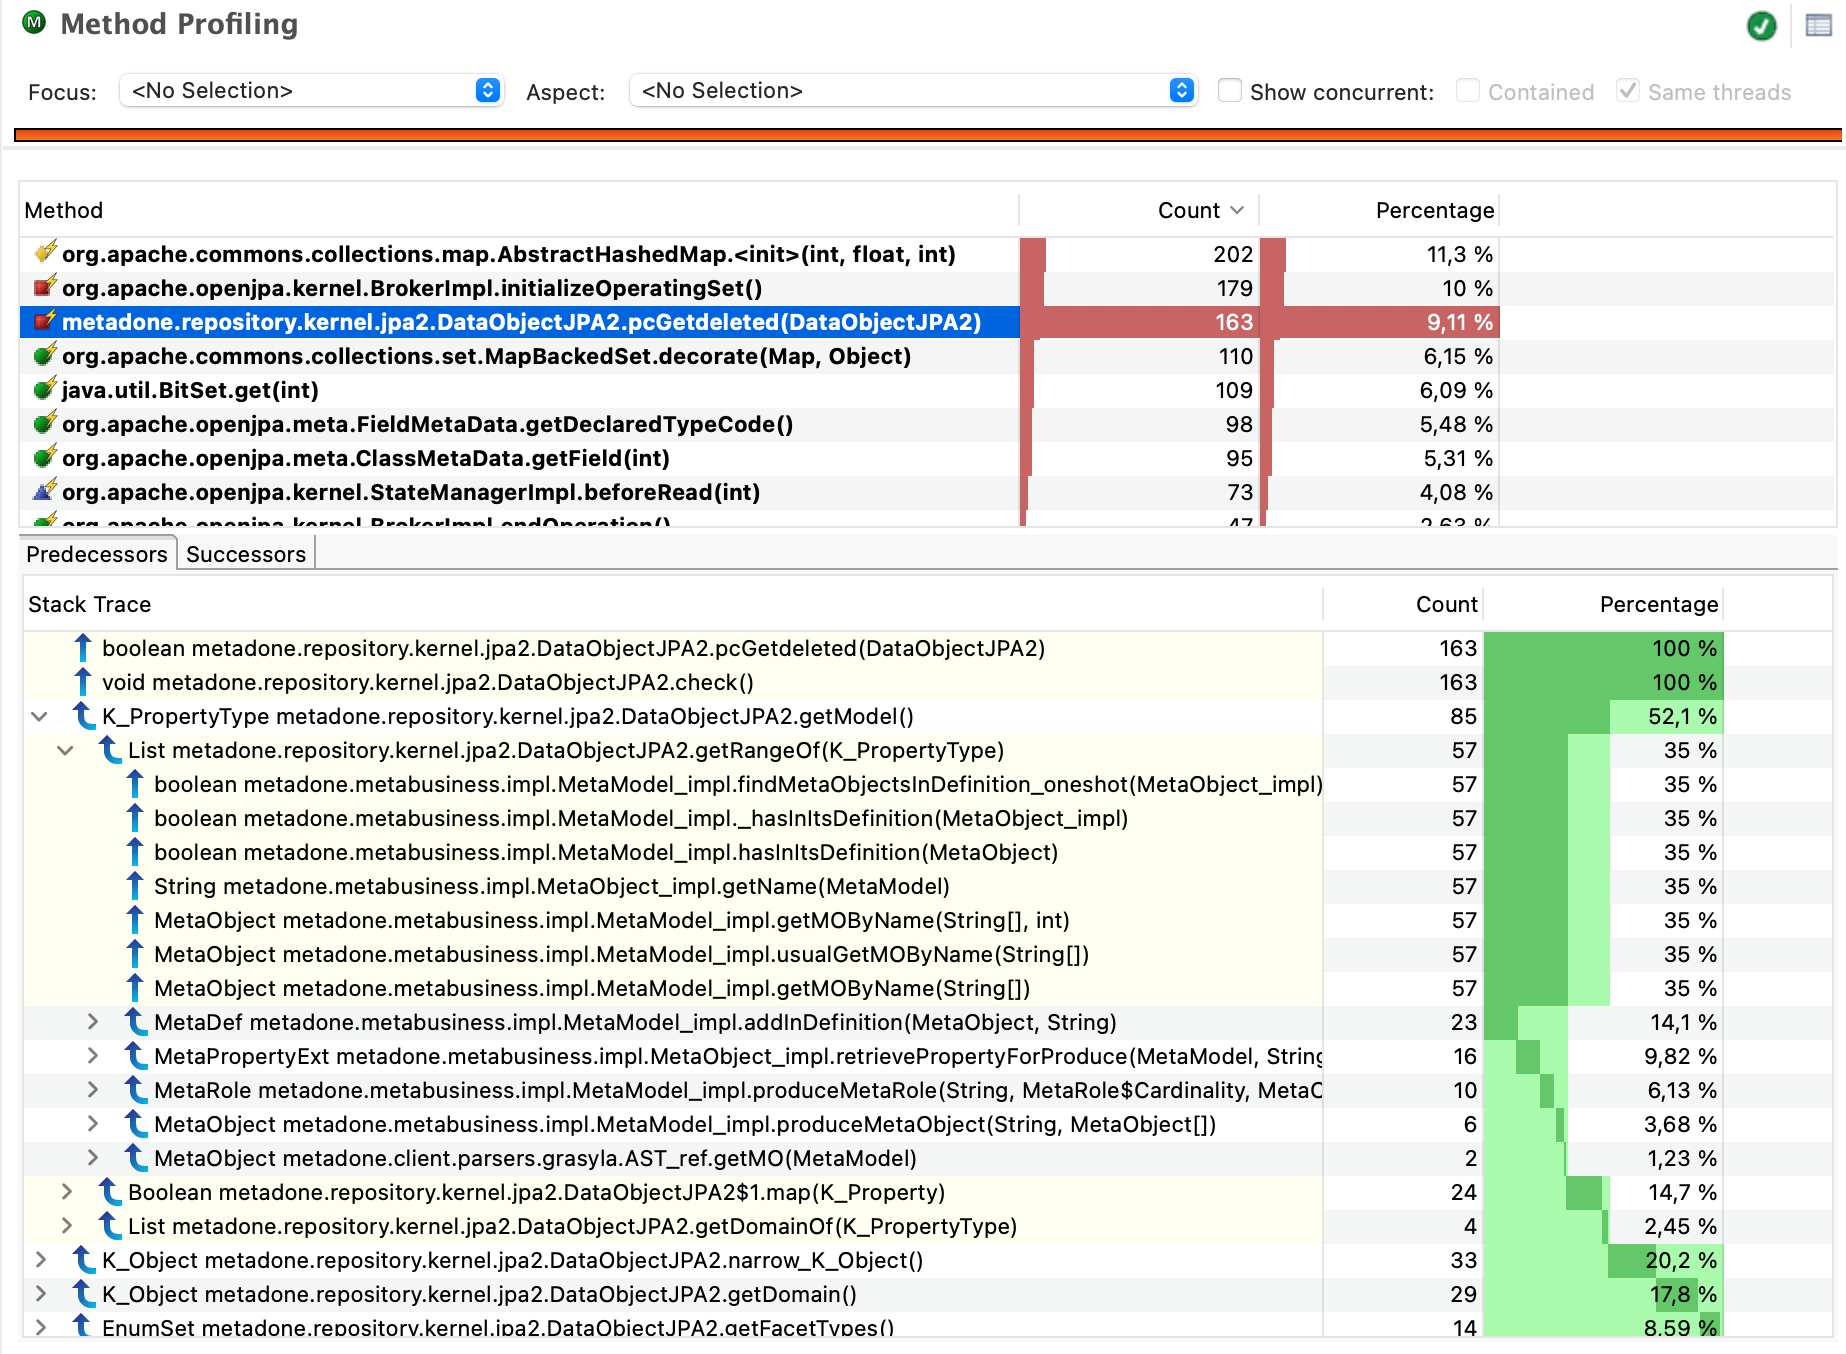
\includegraphics[width=0.8\textwidth]{img/scenario1/jfr-1.png}
\caption{Java Mission Control --- Method Profiling. La méthode
\texttt{pcGetdeleted} (bundle \texttt{metadone\_bundle\_repository\_jpa2})
domine avec 9,11\% des échantillons.}
\label{fig:jfr-1}
\end{figure}

La remontée des prédécesseurs dans JMC reconstruit la \textbf{chaîne
d'appels critique}~:

\begin{center}
\texttt{pcGetdeleted} $\leftarrow$
\texttt{check} $\leftarrow$ 
\texttt{getModel} $\leftarrow$
\texttt{getRangeOf} $\leftarrow$ 
\texttt{findMetaObjectsInDefinition\_oneshot} $\leftarrow$
\texttt{\_hasInItsDefinition} $\leftarrow$
\texttt{hasInItsDefinition} $\leftarrow$
\texttt{...}
\end{center}

Les quatre premières méthodes appartiennent à la couche repository et les suivantes à la couche metabusiness. Avant
d'en analyser le code, nous utilisons async-profiler pour valider et
affiner ce diagnostic.

% -----------------------------------------------
\subsubsection{Analyse approfondie via flamegraph}
% -----------------------------------------------

Async-profiler est lancé en parallèle de JFR selon la configuration
décrite à la section~\ref{sec:env}. Le flamegraph global
(figure~\ref{fig:prof1-flame1}) offre une vue d'ensemble de la répartition
du CPU sur l'ensemble de la phase de démarrage.

\begin{wrapfigure}{r}{5.5cm}
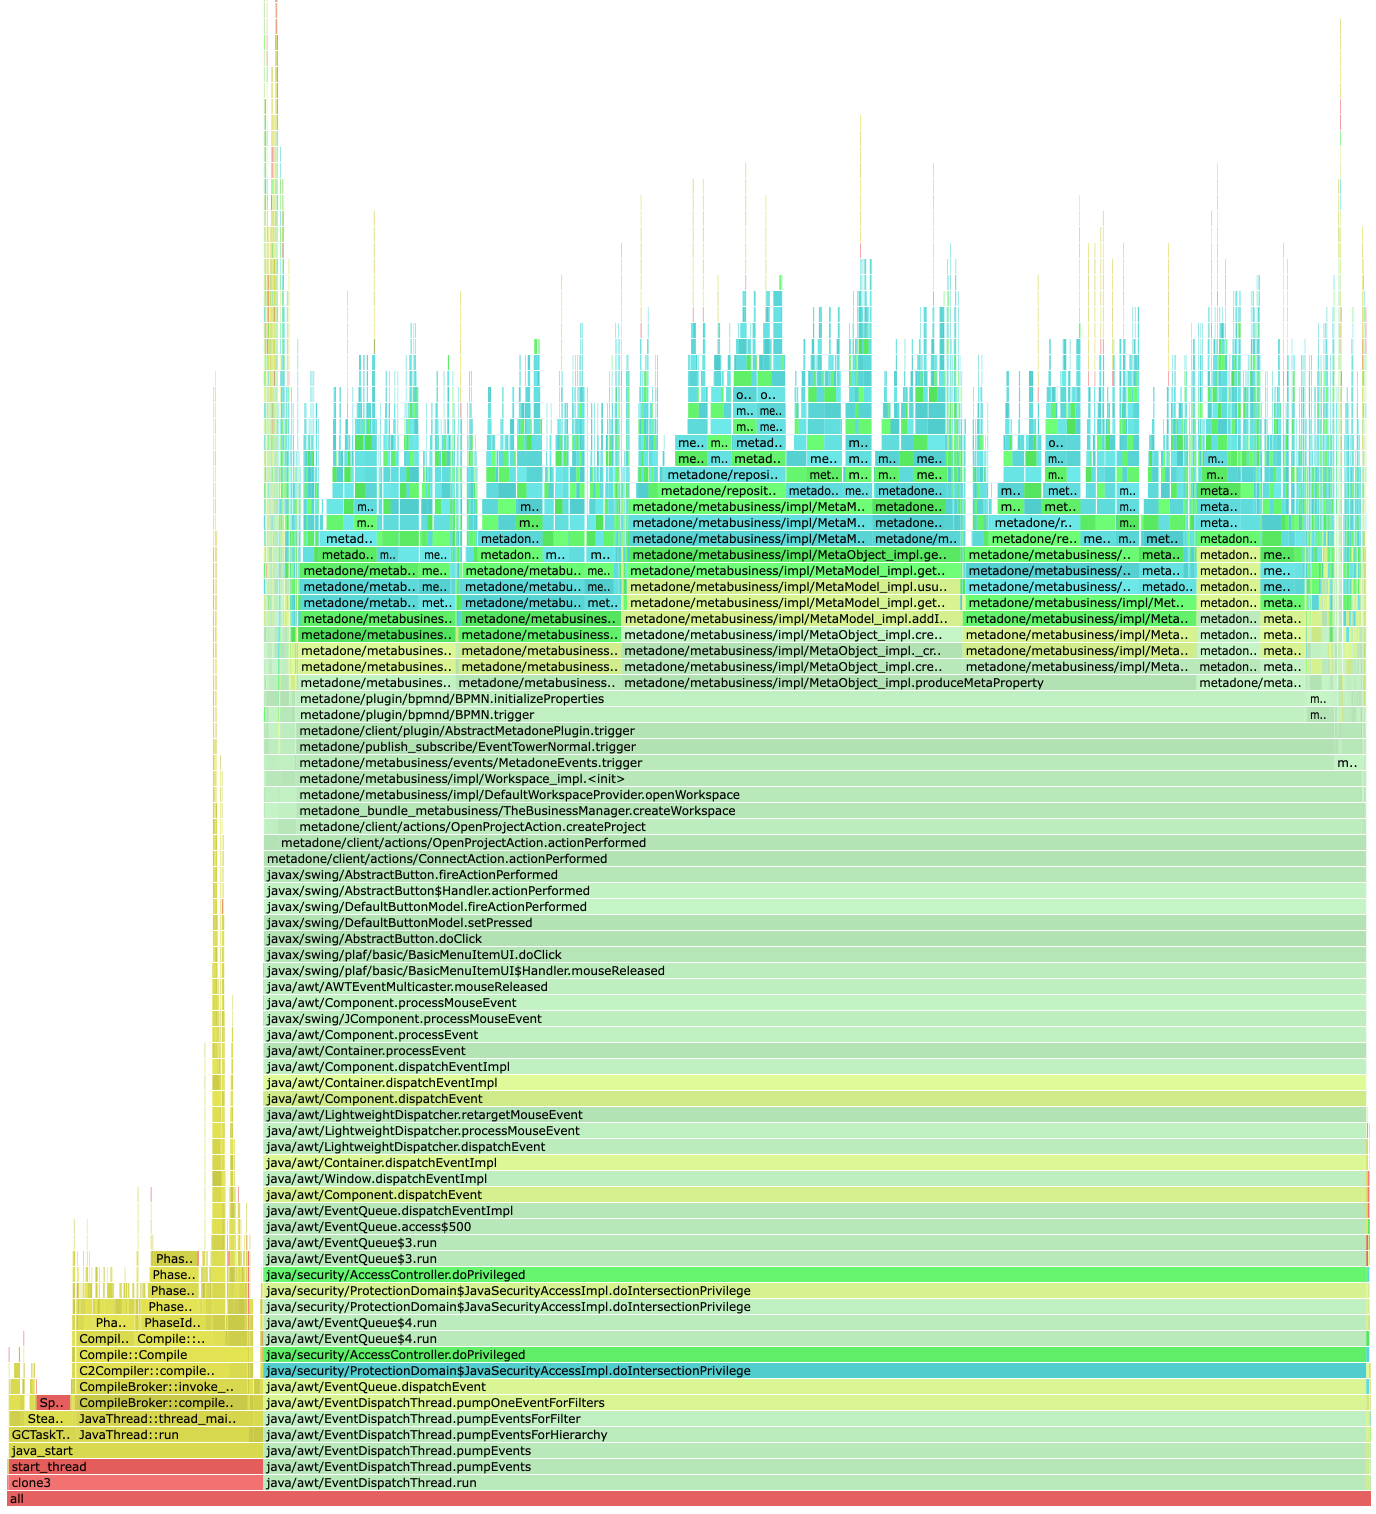
\includegraphics[width=5.5cm]{img/scenario1/prof1/flame1.png}
\caption{Flamegraph global de la phase d'initialisation.}
\label{fig:prof1-flame1}
\end{wrapfigure}

Rappelons la lecture d'un flamegraph~: l'axe vertical représente la
profondeur de pile --- plus on monte, plus on s'approche de la méthode
terminale effectivement exécutée. L'axe horizontal, trié alphabétiquement,
représente le temps CPU total passé dans chaque méthode et ses appelées~:
un rectangle large signale un hotspot.

En se concentrant sur les méthodes identifiées par JFR, les pourcentages
d'occupation CPU lors du démarrage sont les suivants~:

\begin{itemize}
    \item \texttt{pcGetdeleted} --- 35,97\%
    \item \texttt{check} --- 38,48\%
    \item \texttt{getModel} --- 35,79\%
    \item \texttt{getRangeOf} --- 29,33\%
    \item \texttt{findMetaObjectsInDefinition\_oneshot} --- 56,44\%
    \item \texttt{\_hasInItsDefinition} --- 56,57\%
    \item ...
\end{itemize}

Ces pourcentages correspondent à la proportion des échantillons CPU dans
lesquels la méthode apparaît dans la pile d'appels. La divergence entre
les 9,11\% rapportés par JFR et les 35--56\% du flamegraph s'explique par
leur différence de portée~: JFR mesure sur la totalité de la session
(y compris les phases I/O et d'attente JVM), tandis qu'async-profiler isole
ici la phase de création du repository.

Pour plus de clarté, les graphes de la figure~\ref{fig:prof1-zoom} isolent la phase d’initialisation du plugin BPMN. Celui-ci constitue le principal goulot d’étranglement, tant par sa durée de chargement que par la densité de ses appels.

\begin{figure}[htbp]
\begin{subfigure}{\textwidth}
    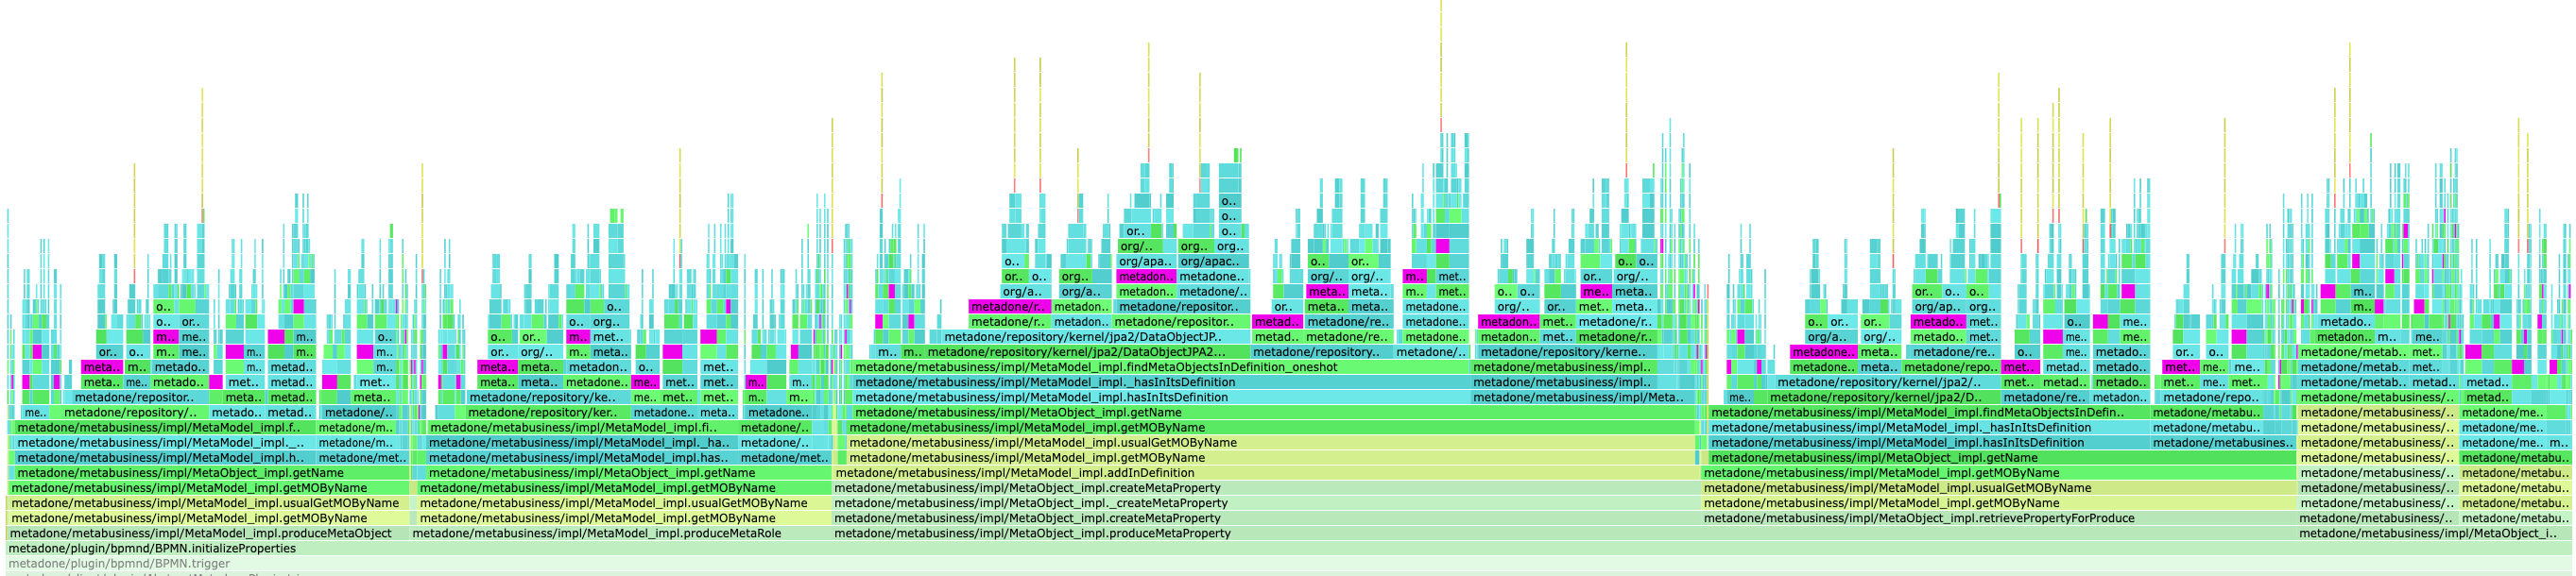
\includegraphics[width=\textwidth]{img/scenario1/prof1/pcGetdeleted.png}
    \caption{\texttt{pcGetdeleted} ---
    bundle \texttt{metadone\_bundle\_repository\_jpa2}}
\end{subfigure}

\medskip
\begin{subfigure}{\textwidth}
    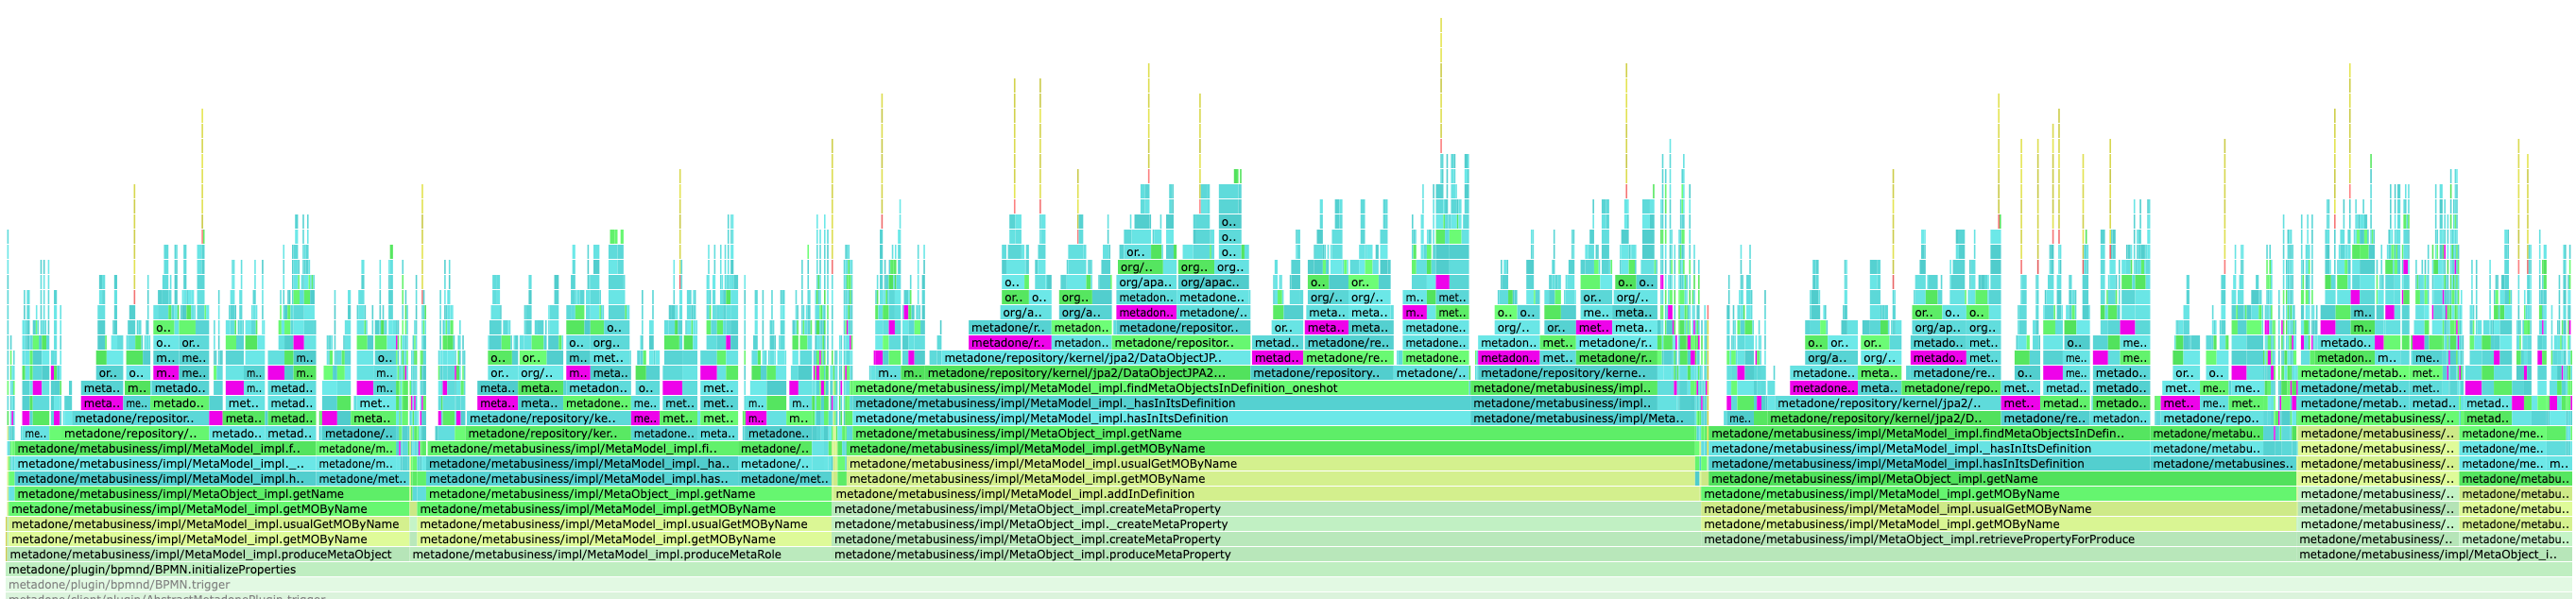
\includegraphics[width=\textwidth]{img/scenario1/prof1/check.png}
    \caption{\texttt{check} ---
    bundle \texttt{metadone\_bundle\_repository\_jpa2}}
\end{subfigure}

\medskip
\begin{subfigure}{\textwidth}
    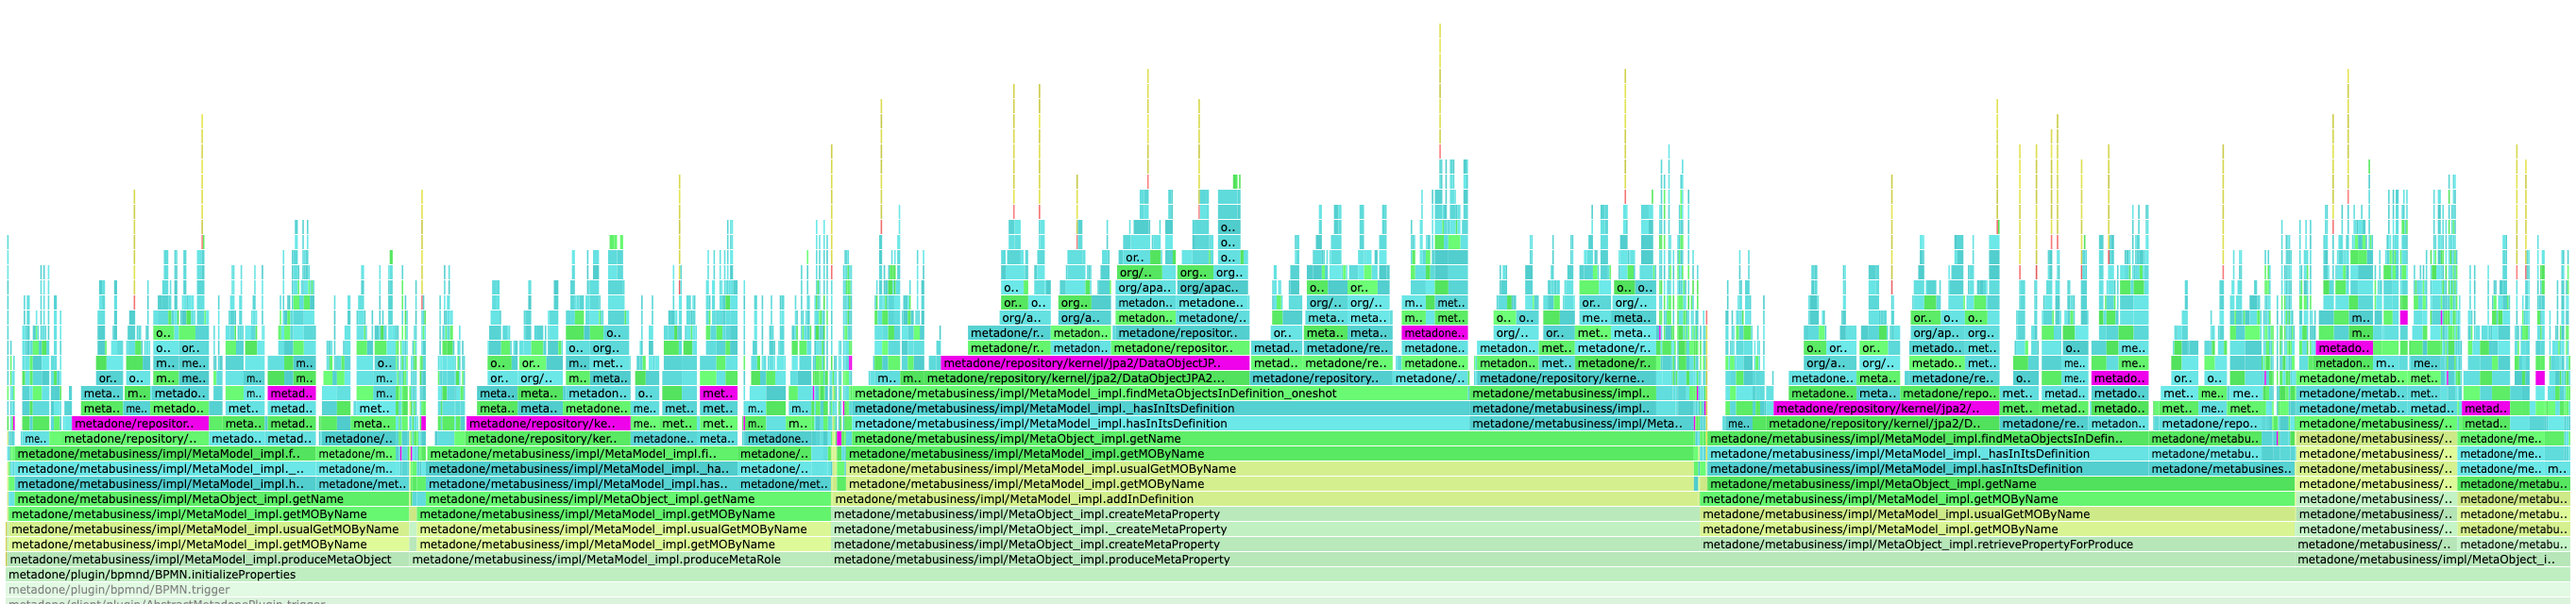
\includegraphics[width=\textwidth]{img/scenario1/prof1/getModel.png}
    \caption{\texttt{getModel} ---
    bundle \texttt{metadone\_bundle\_repository\_jpa2}}
\end{subfigure}

\medskip
\begin{subfigure}{\textwidth}
    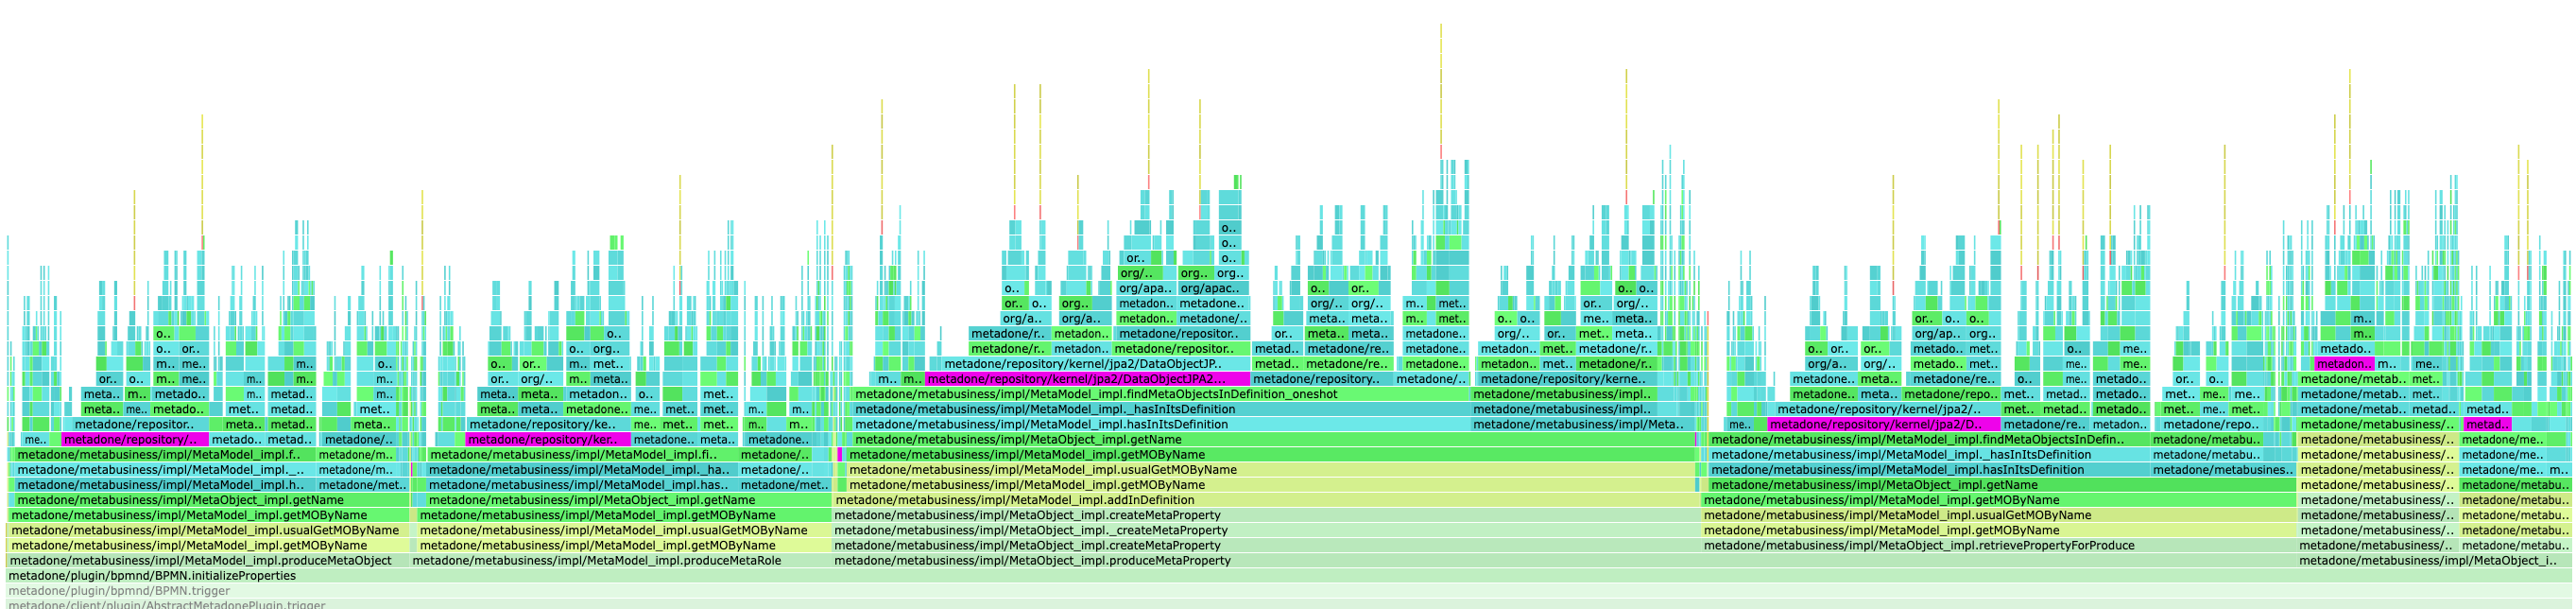
\includegraphics[width=\textwidth]{img/scenario1/prof1/getRangeOf.png}
    \caption{\texttt{getRangeOf} --- 
    bundle \texttt{metadone\_bundle\_repository}}
\end{subfigure}

\medskip
\begin{subfigure}{\textwidth}
    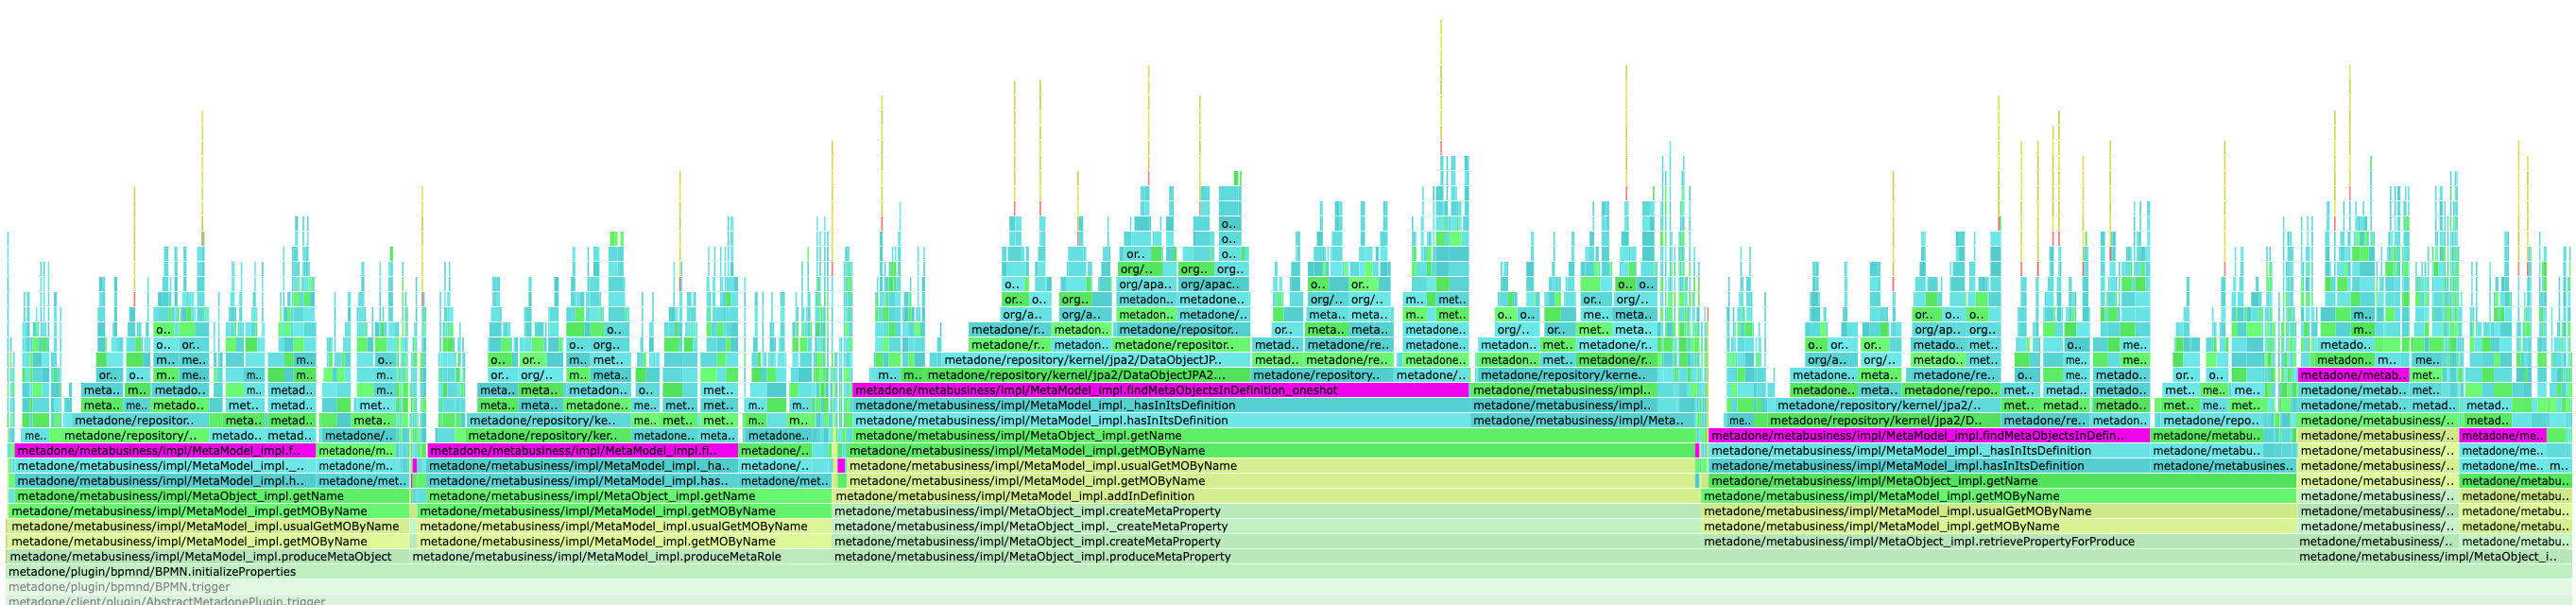
\includegraphics[width=\textwidth]{img/scenario1/prof1/oneshot.png}
    \caption{\texttt{findMetaObjectsInDefinition\_oneshot} --- classe \texttt{MetaModel\_impl}, bundle \texttt{metadone\_bundle\_metabusiness}}
\end{subfigure}

\caption{Flamegraphs isolant la phase d'initialisation du plugin BPMN.}
\label{fig:prof1-zoom}
\end{figure}

Le flamegraph révèle que \texttt{findMetaObjectsInDefinition\_oneshot} est
la méthode terminale d'une pile d'appels extrêmement coûteuse, représentant
plus de 56\% de l'utilisation CPU sur cette phase.

% -----------------------------------------------
\subsubsection{Analyse statique du code et quantification des appels}
% -----------------------------------------------

Afin de confirmer le diagnostic du profilage, nous avons procédé à une
analyse statique du code source couplée à une instrumentation manuelle par
compteurs d'appels. Les mesures confirment une amplification significative~:
pour 1~400 exécutions de \texttt{\_hasInItsDefinition}
(\texttt{MetaModel\_impl}, bundle \texttt{metadone\_bundle\_metabusiness}),
on dénombre plus de 80~000 appels à
\texttt{findMetaObjectsInDefinition\_oneshot}, soit un \textbf{facteur
multiplicatif moyen de 57}.

La cause de cette amplification réside dans la structure de \texttt{\_hasInItsDefinition} (Listing~\ref{ls-has})~: chaque invocation appelle \texttt{findMetaObjectsInDefinition\_oneshot} pour le \texttt{MetaModel} courant (ligne 180), puis pour chacun de ses supertypes \texttt{MetaModel} (ligne 183), multipliant les invocations avec la profondeur de la hiérarchie. Cette hiérarchie est précisément rendue possible par la réflexivité de MetaL$_2$~: \texttt{MetaModel} étend \texttt{MetaObject} (section~\ref{sec:metal2}), si bien que les supertypes d'un \texttt{MetaModel} sont eux-mêmes des \texttt{MetaModel} et déclenchent à leur tour la récursion.

\begin{lstlisting}[firstnumber=174,
  caption={Méthode \texttt{\_hasInItsDefinition} ---
  classe \texttt{MetaModel\_impl},
  bundle \texttt{metadone\_bundle\_metabusiness}},
  label={ls-has}]
private boolean _hasInItsDefinition(MetaObject_impl mo) {
    try {
        final Set<MetaObject> found =
            cache_getMetaObjectsInDefinition
                .isCachedNotNull(mo.getTarget()
                    .getDataObject().getOID());
        if (found != null && found.contains(mo)) {
            return true;
        } else {
            if (this.findMetaObjectsInDefinition_oneshot(mo)) {
                return true;
            } else {
                for (final MetaObject supertype : getAllSupertypes()) {
                    if (supertype.isA(MetaModel.class)) {
                        final MetaModel_impl mm =
                            supertype.narrow(MetaModel_impl.class);
                        if (mm.findMetaObjectsInDefinition_oneshot(mo)) {
                            return true;
                        }
                    }
                }
            }
            return false;
        }
    } catch (final BadPreCondition e) {
        throw new Metal2Exception(e);
    }
}
\end{lstlisting}

La méthode \texttt{findMetaObjectsInDefinition\_oneshot}
(Listing~\ref{ls-oneshot}) répond à une question précise~: le
\texttt{MetaObject} \texttt{partSide} appartient-il directement à la
définition du \texttt{MetaModel} \texttt{this}~?

Pour le comprendre, il faut rappeler comment l'appartenance d'un \texttt{MetaObject} à un \texttt{MetaModel} est encodée dans le kernel~: lors de l'ajout d'un \texttt{MetaObject} à la définition d'un \texttt{MetaModel}, une \texttt{K\_PropertyType} de type \texttt{def\_pt} est créée, reliant le \texttt{MetaObject} (domaine)
au \texttt{MetaModel} (range). La méthode itère donc sur l'ensemble des
propriétés de type \texttt{def\_pt} dont le \texttt{MetaModel} courant est
le range (ligne 204) --- c'est-à-dire toutes les relations d'appartenance
pointant vers ce modèle --- et vérifie pour chacune que son domaine est le
\texttt{MetaObject} recherché (ligne 206). Il s'agit d'une \textbf{recherche
linéaire de complexité $O(n)$}, où $n$ est le nombre de \texttt{MetaObject}
dans la définition du \texttt{MetaModel} considéré.

Cette recherche repose sur \texttt{getRangeOf()} de l'interface
\texttt{K\_Object} (bundle \texttt{metadone\_bundle\_repository}), qui retourne la liste des propriétés dont
l'objet est le range~: c'est l'opération de traversée du graphe de
\texttt{DataObject} qui apparaît au bas du flamegraph et représente
29,33\% du CPU.

\begin{lstlisting}[firstnumber=199,
  caption={Méthode \texttt{findMetaObjectsInDefinition\_oneshot} ---
  classe \texttt{MetaModel\_impl},
  bundle \texttt{metadone\_bundle\_metabusiness}},
  label={ls-oneshot}]
private final boolean findMetaObjectsInDefinition_oneshot(
        MetaObject_impl partSide) {
    try {
        final K_ObjectType wholeSide = this.getTarget();
        final K_ObjectType partSide_o = partSide.getTarget();
        final K_PropertyType defIsDependentOf_pt =
            getWorkspace().getDefIsDependentOf_pt();
        for (final K_Property def_p :
                wholeSide.getRangeOf(workspace.getDef_pt())) {
            final K_Object def_o =
                def_p.getDataObject().narrow_K_Object();
            if (def_o != null &&
                    def_o.getDomainOfIter(defIsDependentOf_pt)
                        .hasNext()) {
                if (def_p.getDomain().equals(partSide_o)) {
                    return true;
                }
            }
        }
        return false;
    } catch (final BadFacet e) {
        throw new Metal2Exception(e);
    } catch (final BadPreCondition e) {
        throw new Metal2Exception(e);
    }
}
\end{lstlisting}

% -----------------------------------------------
\subsubsection{Synthèse du diagnostic}
% -----------------------------------------------

Le goulot d'étranglement ne provient pas d'un algorithme intrinsèquement
complexe, mais de l'accumulation de recherches linéaires répétées dans des
boucles imbriquées.
La pile d'appels problématique est la suivante~:

\begin{center}
\small
\texttt{MetaModel\_impl.\_hasInItsDefinition} \\
(itération sur les supertypes via \texttt{getAllSupertypes()}) \\[4pt]
$\downarrow$ \\[4pt]
\texttt{MetaModel\_impl.findMetaObjectsInDefinition\_oneshot} \\
(itération $O(n)$ sur les propriétés \texttt{def\_pt}) \\[4pt]
$\downarrow$ \\[4pt]
\texttt{K\_Object.getRangeOf} --- \texttt{metadone\_bundle\_repository} \\
(traversée du graphe de \texttt{DataObject}, 29,33\% CPU)
\end{center}

La mitigation naturelle est la \textbf{mémoïsation}~: si l'appartenance
d'un \texttt{MetaObject} à un \texttt{MetaModel} est déjà connue, la
traversée du graphe est superflue. Un mécanisme de cache existe dans le
code --- \texttt{cache\_getMetaObjectsInDefinition}, instance de
\texttt{CacheCallFunction} du bundle \texttt{metadone\_common} --- mais il est rendu inopérant par deux défauts cumulés~:

\begin{enumerate}
    \item \textbf{Cache désactivé à l'initialisation.} Le paramètre
    \texttt{false} passé au constructeur de \texttt{CacheCallFunction}
    désactive globalement le cache. Chaque appel à
    \texttt{\_hasInItsDefinition} court-circuite le cache et déclenche
    une traversée complète, quelle que soit la fréquence de la même
    requête.

    \item \textbf{Inversion de clé.} Lors de la consultation du cache,
    l'OID utilisé est celui du \texttt{MetaObject} recherché (\texttt{mo}),
    alors que le cache est indexé par OID de \texttt{MetaModel}
    (\texttt{this}). Même si le cache avait été activé, cette inversion
    garantissait une absence systématique de correspondance, rendant le
    cache indiscernable d'une absence totale.
\end{enumerate}

Ces deux défauts conjugués expliquent le facteur multiplicatif de 57
observé. La phase d'optimisation s'articulera autour de deux axes
complémentaires~: la correction du cache existant, et la substitution des
recherches linéaires par des structures d'accès en $O(1)$, présentés à la
section suivante.
\subsection{Optimisation de \texttt{MetaModel\_impl}}
\label{sec:opti-metamodel}

Les trois optimisations présentées dans cette section ciblent toutes la
classe \texttt{MetaModel\_impl} du bundle \texttt{metadone\_bundle\_metabusiness}.
Elles forment une séquence logique~: la première répare le mécanisme de
cache existant mais inopérant, la deuxième élimine une redondance
algorithmique indépendante du cache, et la troisième rend le cache
efficace pendant le bootstrapping en remplaçant sa stratégie d'invalidation
par une mise à jour incrémentale.

% -------------------------------------------------------------------
\subsubsection{Optimisation~1 : activation du cache et correction de
la clé}
% -------------------------------------------------------------------

L'analyse a révélé que le mécanisme de cache de \texttt{MetaModel\_impl}
était doublement inopérant~: désactivé par construction, et erroné dans
sa gestion des clés. Ces deux défauts ont été corrigés conjointement.

%\paragraph{Activation du cache.}
La classe utilitaire \texttt{CacheCallFunction<Arg,~Ret>} du bundle
\texttt{metadone\_common} associe
à chaque argument une valeur de retour dans une \texttt{HashMap} interne.
Elle accepte un paramètre booléen à la construction qui active ou désactive
ce mécanisme~: lorsqu'il vaut \texttt{false}, chaque appel à
\texttt{isCachedNotNull} retourne systématiquement \texttt{null}, rendant
le cache inopérant sans aucune indication visible à l'appelant. Dans
\texttt{MetaModel\_impl}, ce paramètre était initialisé à \texttt{false},
désactivant globalement le cache de \texttt{getMetaObjectsInDefinition}.
Le premier correctif consiste à passer ce paramètre à \texttt{true}
(figure~\ref{fig:opti-1-cache}).

\begin{figure}[h]
\centering
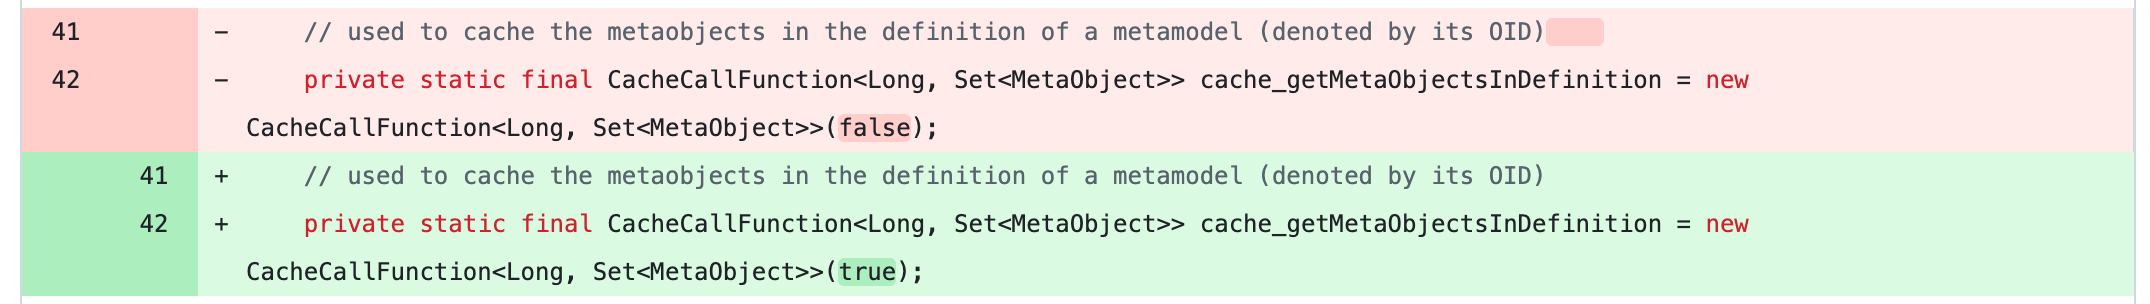
\includegraphics[width=0.9\textwidth]{img/scenario1/opti-1-cache.png}
\caption{Activation du cache \texttt{cache\_getMetaObjectsInDefinition}
dans \texttt{MetaModel\_impl} --- bundle
\texttt{metadone\_bundle\_metabusiness}.}
\label{fig:opti-1-cache}
\end{figure}

%\paragraph{Correction de la clé d'accès.}
Le second défaut porte sur la clé utilisée lors de la consultation du
cache dans \texttt{\_hasInItsDefinition}. \texttt{CacheCallFunction} indexe
ses entrées par l'OID du \texttt{DataObject} sous-jacent : dans ce contexte, la clé naturelle est
l'OID du \texttt{MetaModel} courant (\texttt{this}), puisque le cache
enregistre \textit{l'ensemble des membres de ce MetaModel}.

Or, le code original passait l'OID du \texttt{MetaObject} \textit{recherché}
(\texttt{mo}) à la place. Cette inversion produisait un \textit{cache miss}
systématique~: même si le cache avait contenu l'entrée attendue, elle
n'aurait jamais été trouvée. Le second correctif substitue donc l'OID de
\texttt{this} à celui de \texttt{mo} (figure~\ref{fig:opti-1-cle}).

\begin{figure}[h]
\centering
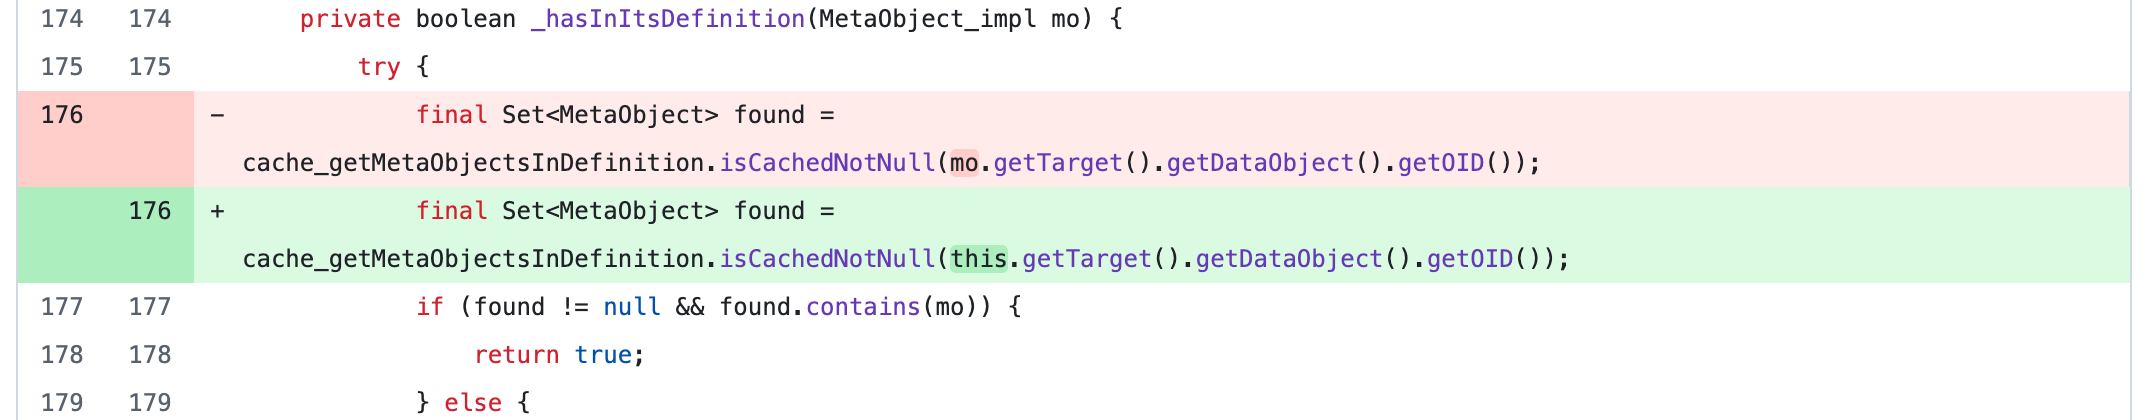
\includegraphics[width=0.9\textwidth]{img/scenario1/opti-1-cle.png}
\caption{Correction de la clé d'accès au cache dans
\texttt{\_hasInItsDefinition} --- l'OID de \texttt{this} (le
\texttt{MetaModel}) se substitue à l'OID de \texttt{mo} (le
\texttt{MetaObject} recherché).}
\label{fig:opti-1-cle}
\end{figure}

%\paragraph{Portée de cette optimisation.}
Ces corrections sont un prérequis logique, mais leur bénéfice est nul
\textit{pendant le bootstrapping}. Lors de la création de la base de
données, les entrées du cache sont systématiquement absentes au moment
où \texttt{\_hasInItsDefinition} est appelé~: chaque appel à
\texttt{\_addInDefinition} invalide le cache avant que le prochain appel
à \texttt{getMetaObjectsInDefinition} ne puisse le peupler. Elles sont
en revanche indispensables pour le bon fonctionnement des optimisations
suivantes, et bénéficient à toutes les requêtes effectuées \textit{après}
le bootstrapping.

% -------------------------------------------------------------------
\subsubsection{Optimisation~2 : suppression de la redondance dans
\texttt{getMOByName}}
% -------------------------------------------------------------------

%\paragraph{Contexte et problème.}
La méthode \texttt{getMOByName} est appelée lors du bootstrapping pour
vérifier l'unicité du nom de chaque nouvel objet ajouté au métamodèle.
Elle itère sur l'ensemble des \texttt{MetaObject} retournés par
\texttt{getMetaObjectsInDefinition()} et, pour chaque élément, invoque
\texttt{mo.getName(this)} afin d'en récupérer le nom.

Conformément au patron \textit{Design by Contract} décrit à la
section~\ref{sec:dbc}, \texttt{getName} est la méthode publique de
l'interface. Avant de déléguer à \texttt{\_getName}, elle effectue deux
vérifications défensives~: un contrôle de nullité, puis une vérification
d'appartenance via \texttt{metamodel.hasInItsDefinition(this)}
(Listing~\ref{ls-getname}, ligne~354--355). Cette précondition appelle à
son tour \texttt{\_hasInItsDefinition}, qui --- sans cache actif ---
déclenche un scan linéaire $O(n)$ via
\texttt{findMetaObjectsInDefinition\_oneshot}.

\begin{lstlisting}[firstnumber=352,
  caption={\texttt{getName} --- méthode publique de \texttt{MetaObject\_impl},
  bundle \texttt{metadone\_bundle\_metabusiness}. La précondition
  ligne~354--355 déclenche un scan $O(n)$ à chaque appel.},
  label={ls-getname}]
@Override
public String getName(MetaModel metamodel) throws BadPreCondition {
    NullArgument.check(metamodel);
    if (!metamodel.hasInItsDefinition(this)) {
        throw new BadPreCondition("Attempt to get the name of a "
            + "metaobject in the context of a metamodel that "
            + "doesn't contain it.");
    }
    try {
        final String result = _getName(metamodel);
        if (result != null) {
            return result;
        }
        throw new Metal2Exception(...);
    } catch (final BadPreCondition e) {
        throw new Metal2Exception(e);
    }
}
\end{lstlisting}

\texttt{\_getName} est la méthode interne qui effectue la recherche
réelle~: elle parcourt les \texttt{ConcreteProperty<String>} associées
au \texttt{MetaObject} et cherche celle définie dans le
\texttt{ConcreteModel} correspondant au \texttt{MetaModel}
(Listing~\ref{ls--getname}, lignes~378--379), puis remonte
récursivement dans les supertypes directs si aucune propriété ne
correspond (ligne~383). Elle ne comporte aucune vérification
d'appartenance.

\begin{lstlisting}[firstnumber=370,
  caption={\texttt{\_getName} --- méthode interne de
  \texttt{MetaObject\_impl}. Pas de vérification d'appartenance~:
  l'invariant est supposé garanti par l'appelant.},
  label={ls--getname}]
private String _getName(MetaModel metamodel) {
    try {
        assert metamodel != null;
        final ConcreteObject thisConcrete = this.narrow2ConcreteObject();
        final ConcreteModel concreteModel =
            metamodel.narrow2ConcreteModel();
        final MetaPropertyExt<String> metaObjectName =
            workspace.getMetaObjectName();
        for (final ConcreteProperty<String> cp :
                thisConcrete.getProperties(metaObjectName)) {
            if (concreteModel.isInDefinition(cp)) {
                return cp.getValue();
            }
        }
        for (final MetaObject mmO : metamodel.getDirectSupertypes()) {
            final MetaModel mm;
            try {
                mm = mmO.narrow(MetaModel.class);
            } catch (final BadPreCondition e) {
                continue;
            }
            final String name = _getName(mm);
            if (name != null) {
                return name;
            }
        }
        return null;
    } catch (final BadPreCondition e) {
        throw new Metal2Exception(e);
    }
}
\end{lstlisting}

%\paragraph{Analyse de la complexité.}
Invoquer \texttt{getName} depuis une boucle sur
\texttt{getMetaObjectsInDefinition()} est structurellement redondant.
Puisque chaque élément \texttt{mo} provient par définition des membres
du \texttt{MetaModel}, la précondition \texttt{hasInItsDefinition(this)}
est toujours vraie et son évaluation est superflue. Sans cache actif, cette
vérification déclenche à chaque itération un parcours de la hiérarchie de
supertypes du \texttt{MetaModel}, chacun de ces supertypes déclenchant à
son tour un scan linéaire dans \texttt{findMetaObjectsInDefinition\_oneshot}.
Le coût cumulé de la boucle est donc~:
\[
\underbrace{O(n)}_{\text{itérations de \texttt{getMOByName}}}
\;\times\;
\underbrace{O(s)}_{\text{supertypes dans \texttt{\_hasInItsDefinition}}}
\;\times\;
\underbrace{O(n)}_{\text{scan dans \texttt{\_oneshot}}}
\;=\; O(n^2 \cdot s)
\]
où $s$ désigne la profondeur de la hiérarchie de supertypes du
\texttt{MetaModel}. La réflexivité de MetaL$_2$ (section~\ref{sec:metal2})
autorise cette profondeur à croître linéairement avec le nombre de
méta-modèles définis~: dans le pire cas, $s = O(n)$, ce qui ramène la
complexité effective à $O(n^3)$ pour la dimension d'appartenance.

%\paragraph{Solution.}
La solution consiste à court-circuiter la méthode publique \texttt{getName}
et à appeler directement \texttt{\_getName}, dont l'invariant d'appartenance
est ici garanti structurellement~: la source des \texttt{MetaObject} est
interne à \texttt{getMOByName}, qui les obtient lui-même via
\texttt{getMetaObjectsInDefinition()}. Pour rendre cet accès possible sans
briser l'encapsulation du bundle, la visibilité de \texttt{\_getName} a été
élargie de \texttt{private} à \textit{package-private}~: les deux classes
\texttt{MetaModel\_impl} et \texttt{MetaObject\_impl} appartenant au même
package, l'accès reste confiné à la couche d'implémentation et invisible
depuis les interfaces publiques de MetaL$_2$.

L'appel est précédé d'un \texttt{narrow(MetaObject\_impl.class)} pour
descendre du type d'interface \texttt{MetaObject} vers l'implémentation
concrète, conformément au patron \textit{Proxy} décrit à la
section~\ref{sec:proxy} (figure~\ref{fig:opti-2}).

\begin{figure}[h]
\centering
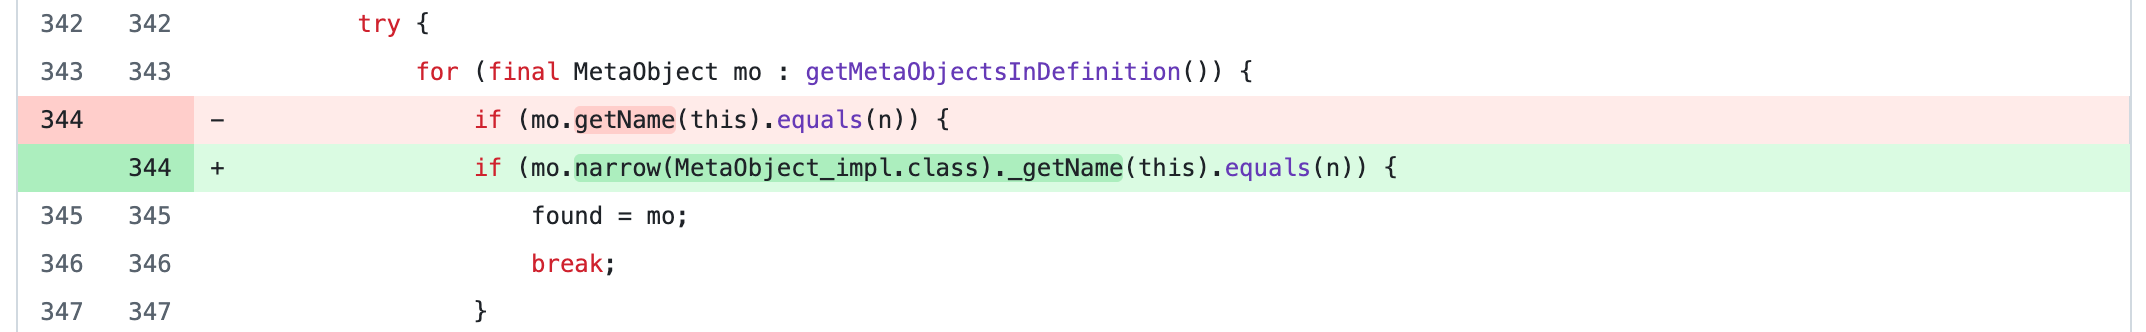
\includegraphics[width=0.9\textwidth]{img/scenario1/opti-2.png}
\caption{Appel direct à \texttt{\_getName} dans \texttt{getMOByName}
--- bundle \texttt{metadone\_bundle\_metabusiness}. Le
\texttt{narrow(MetaObject\_impl.class)} descend du type d'interface
vers l'implémentation concrète selon le patron Proxy.}%(section~\ref{sec:proxy})
\label{fig:opti-2}
\end{figure}

Chaque itération de la boucle passe d'un coût $O(n)$ à un coût
quasi-constant, ramenant le coût cumulé du bootstrapping de $O(n^3)$ à
$O(n^2)$. Notons que le bootstrapping reste $O(n^2)$~: il est nécessaire
de vérifier l'unicité du nom de chaque nouvel objet par rapport aux $n$
objets déjà présents, mais la troisième dimension de complexité --- le
scan d'appartenance --- est supprimée.

Comme le montre la figure~\ref{fig:ouverture-2}, cette seule optimisation divise le temps de création du repository par environ quatre (18\,198~ms $\rightarrow$ 4\,560~ms en médiane, CV~$=$~0,7\,\%).

\begin{figure}[h]
\centering
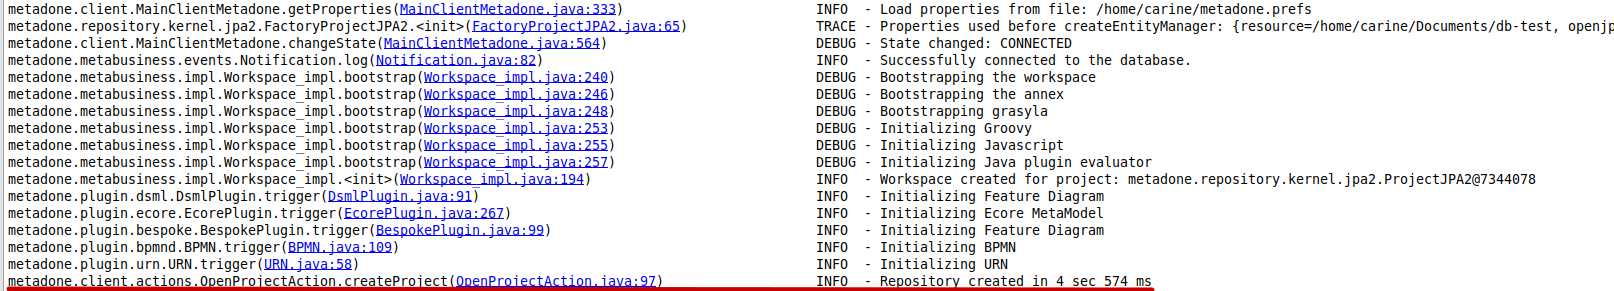
\includegraphics[width=0.9\textwidth]{img/scenario1/ouverture-2.png}
\caption{Temps de création du repository après l'optimisation~2~:
médiane à 4\,560~ms (CV~$=$~0,7\,\%), soit un facteur de réduction de~$\times$\,4,0 par rapport à la baseline de 18\,198~ms.}
\label{fig:ouverture-2}
\end{figure}

% -------------------------------------------------------------------
\subsubsection{Optimisation~3 : mise à jour incrémentale du cache dans
\texttt{\_addInDefinition}}
% -------------------------------------------------------------------

%\paragraph{Problème résiduel.}
Malgré l'activation du cache (optimisation~1), celui-ci reste inefficace
pendant le bootstrapping. La raison est la stratégie d'invalidation
appliquée dans \texttt{\_addInDefinition}~: chaque ajout d'un
\texttt{MetaObject} à la définition d'un \texttt{MetaModel} efface
l'entrée de cache correspondante. Pendant le bootstrapping, où des centaines
d'objets sont ajoutés séquentiellement, cette stratégie condamne le cache
à rester perpétuellement vide~: chaque invalidation supprime l'entrée avant
que le prochain appel à \texttt{getMetaObjectsInDefinition} ne puisse
l'exploiter. Tout appel à \texttt{\_hasInItsDefinition} déclenche donc
toujours un scan $O(n)$ via \texttt{findMetaObjectsInDefinition\_oneshot},
sans jamais bénéficier du cache.

%\paragraph{Solution.}
Le correctif consiste à remplacer la stratégie d'\textbf{invalidation} par
une stratégie de \textbf{mise à jour incrémentale}. La méthode
\texttt{isCached} de \texttt{CacheCallFunction} retourne une paire
\texttt{(Boolean,~Set<MetaObject>)} indiquant si une entrée de cache existe
pour ce \texttt{MetaModel} et, le cas échéant, l'ensemble des membres déjà
mis en cache. Deux cas sont alors distingués (figure~\ref{fig:opti-3})~:

\begin{itemize}
    \item \textbf{Le cache existe}~: le nouvel objet est inséré directement
    dans l'ensemble en mémoire en $O(1)$, maintenant l'invariant du cache
    sans aucun scan supplémentaire.
    \item \textbf{Le cache n'existe pas encore}~: aucune action n'est
    entreprise. Le cache est construit de manière \textit{paresseuse}~:
    c'est le prochain appel à \texttt{getMetaObjectsInDefinition} qui
    effectuera le scan complet et construira l'entrée initiale, en incluant
    tous les objets déjà présents à ce moment.
\end{itemize}

\begin{figure}[h]
\centering
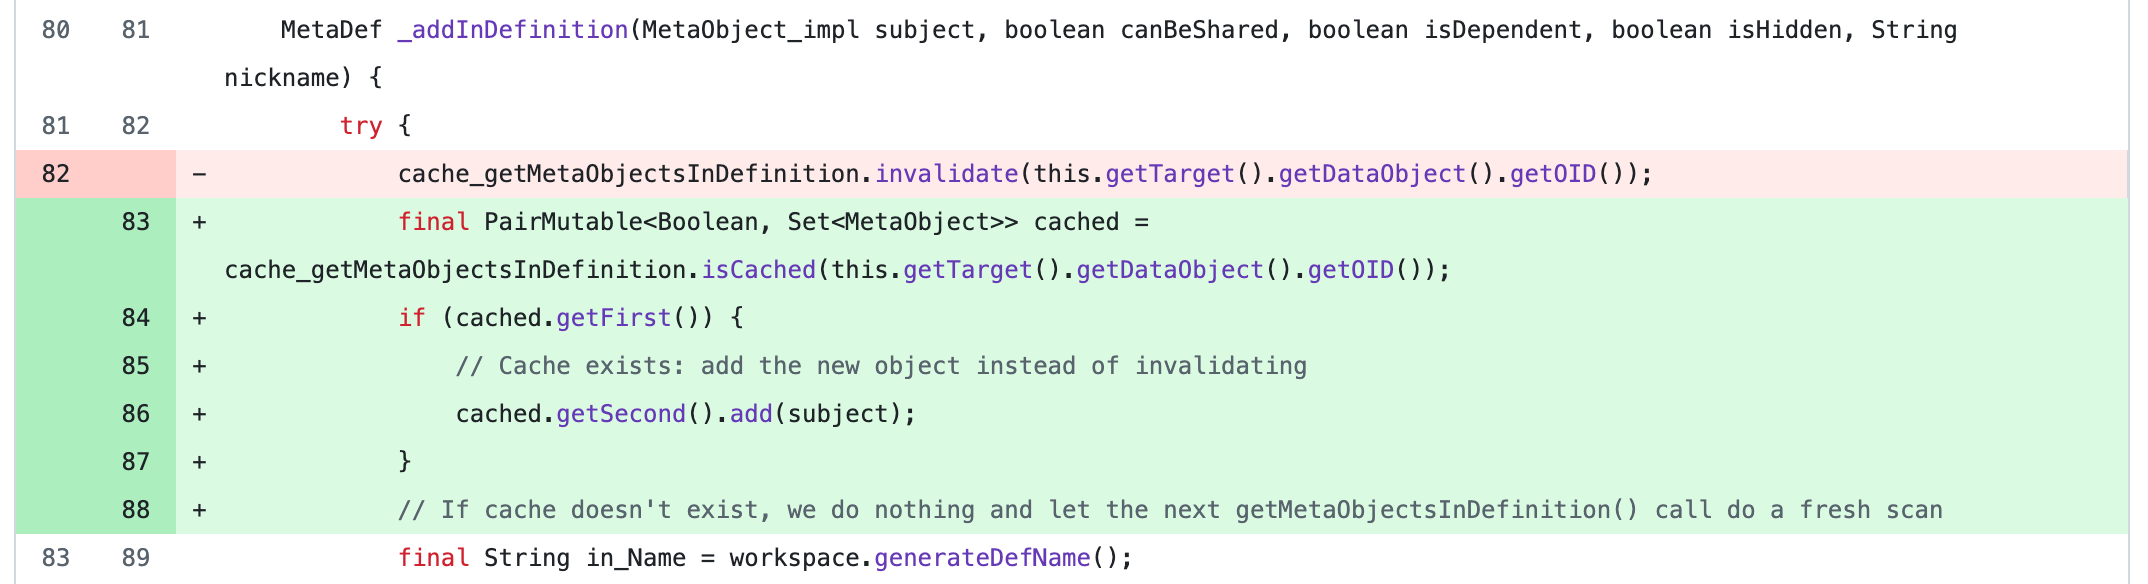
\includegraphics[width=0.9\textwidth]{img/scenario1/opti-3.png}
\caption{Mise à jour incrémentale du cache dans
\texttt{\_addInDefinition} --- bundle
\texttt{metadone\_bundle\_metabusiness}. Deux branches~: insertion
$O(1)$ si le cache existe, initialisation paresseuse sinon.}
\label{fig:opti-3}
\end{figure}

%\paragraph{Correction de la stratégie.}
Cette approche est correcte car l'ensemble mis en cache représente
exactement les membres de la définition du \texttt{MetaModel}~: lors d'un
ajout, on connaît précisément l'élément à insérer, ce qui suffit à maintenir
la cohérence sans reconstruire l'ensemble. La stratégie d'initialisation
paresseuse garantit par ailleurs qu'aucun cache partiellement construit
n'est jamais consulté~: soit le cache est complet (construit par un appel
antérieur à \texttt{getMetaObjectsInDefinition}), soit il est absent et
sera reconstruit à la demande.

%\paragraph{Interaction avec l'optimisation~1.}
Cette optimisation ne peut fonctionner correctement que si le cache est
activé (optimisation~1) et que la clé utilisée est la bonne. Les trois
optimisations forment donc une chaîne dépendante~: l'optimisation~1 est
un prérequis pour que les optimisations~2 et~3 aient un effet, et
l'optimisation~3 est ce qui rend le cache efficace \textit{pendant} le
bootstrapping plutôt que seulement après.

La combinaison des trois optimisations transforme les scans $O(n)$
répétés en de simples insertions et lectures mémoire $O(1)$, réduisant
la complexité algorithmique du bootstrapping de $O(n^3)$ à $O(n^2)$
pour la dimension d'appartenance.

\subsection{Tests de performance}
\label{sec:scenario1-tests1}

Conformément au cycle décrit à la section~\ref{sec:cycle}, les
optimisations implémentées sont évaluées par comparaison avec la
\textit{baseline} établie à la section~\ref{sec:scenario1}
(18~198~ms). Deux dimensions sont mesurées~: le \textbf{volume d'appels}
dans la chaîne critique (via l'instrumentation manuelle par compteurs),
et le \textbf{profil CPU} après optimisation (via JFR et async-profiler).

% -----------------------------------------------
\subsubsection{Réduction du volume d'appels}
% -----------------------------------------------

Le tableau~\ref{tab:appels-opti1} résume l'évolution du nombre d'appels
dans la chaîne critique pour une charge de travail identique (bootstrapping
complet du repository avec le plugin BPMN).

\begin{table}[h]
\centering
\caption{Évolution du volume d'appels dans la chaîne critique ---
bootstrapping complet du repository.}
\label{tab:appels-opti1}
\begin{tabular}{lrrr}
\hline
\textbf{Méthode} & \textbf{Avant} & \textbf{Après} &
\textbf{Réduction} \\
\hline
\texttt{\_hasInItsDefinition} & $\sim$1~400 & $\sim$650 & $\sim$54\% \\
\texttt{findMetaObjectsInDefinition\_oneshot} & $\sim$80~000 & $\sim$750 &
$\sim$99\% \\
\hline
\end{tabular}
\end{table}

La réduction de 54\% des appels à \texttt{\_hasInItsDefinition} est la
conséquence directe de l'\textbf{optimisation~1}~: le cache étant désormais
opérationnel avec la bonne clé, une fraction significative des vérifications
d'appartenance est court-circuitée dès que l'information est disponible en
mémoire, sans traversée du graphe.

L'impact le plus massif est celui de l'\textbf{optimisation~2}~: la chute
de 99\% des appels à \texttt{findMetaObjectsInDefinition\_oneshot} confirme
que la suppression de la précondition dans \texttt{getMOByName} a brisé la
boucle quadratique. Le système ne répercute plus un scan $O(n)$ sur chaque
accès au nom d'un objet~; la troisième dimension de complexité est
éliminée.

L'\textbf{optimisation~3} contribue au reliquat~: grâce à la mise à jour incrémentale, les appels qui atteignent encore \texttt{\_hasInItsDefinition} sont servis en $O(1)$ depuis le cache au lieu de redéclencher un parcours complet de \texttt{getRangeOf}.

% -----------------------------------------------
\subsubsection{Profilage post-optimisation avec JFR}
% -----------------------------------------------

La figure~\ref{fig:jfr-2} montre le Method Profiling JMC après
optimisation. Le compteur d'échantillons pour la chaîne critique est passé
de 163 à 28, et \texttt{getModel} --- qui dominait avec 52,1\% des
échantillons CPU --- n'en représente plus que 7,14\%. Ces chiffres
confirment que le goulot d'étranglement identifié à la
section~\ref{sec:scenario1-profil1} a été résolu~: la méthode n'apparaît
plus en tête du classement de charge.

\begin{figure}[h]
\centering
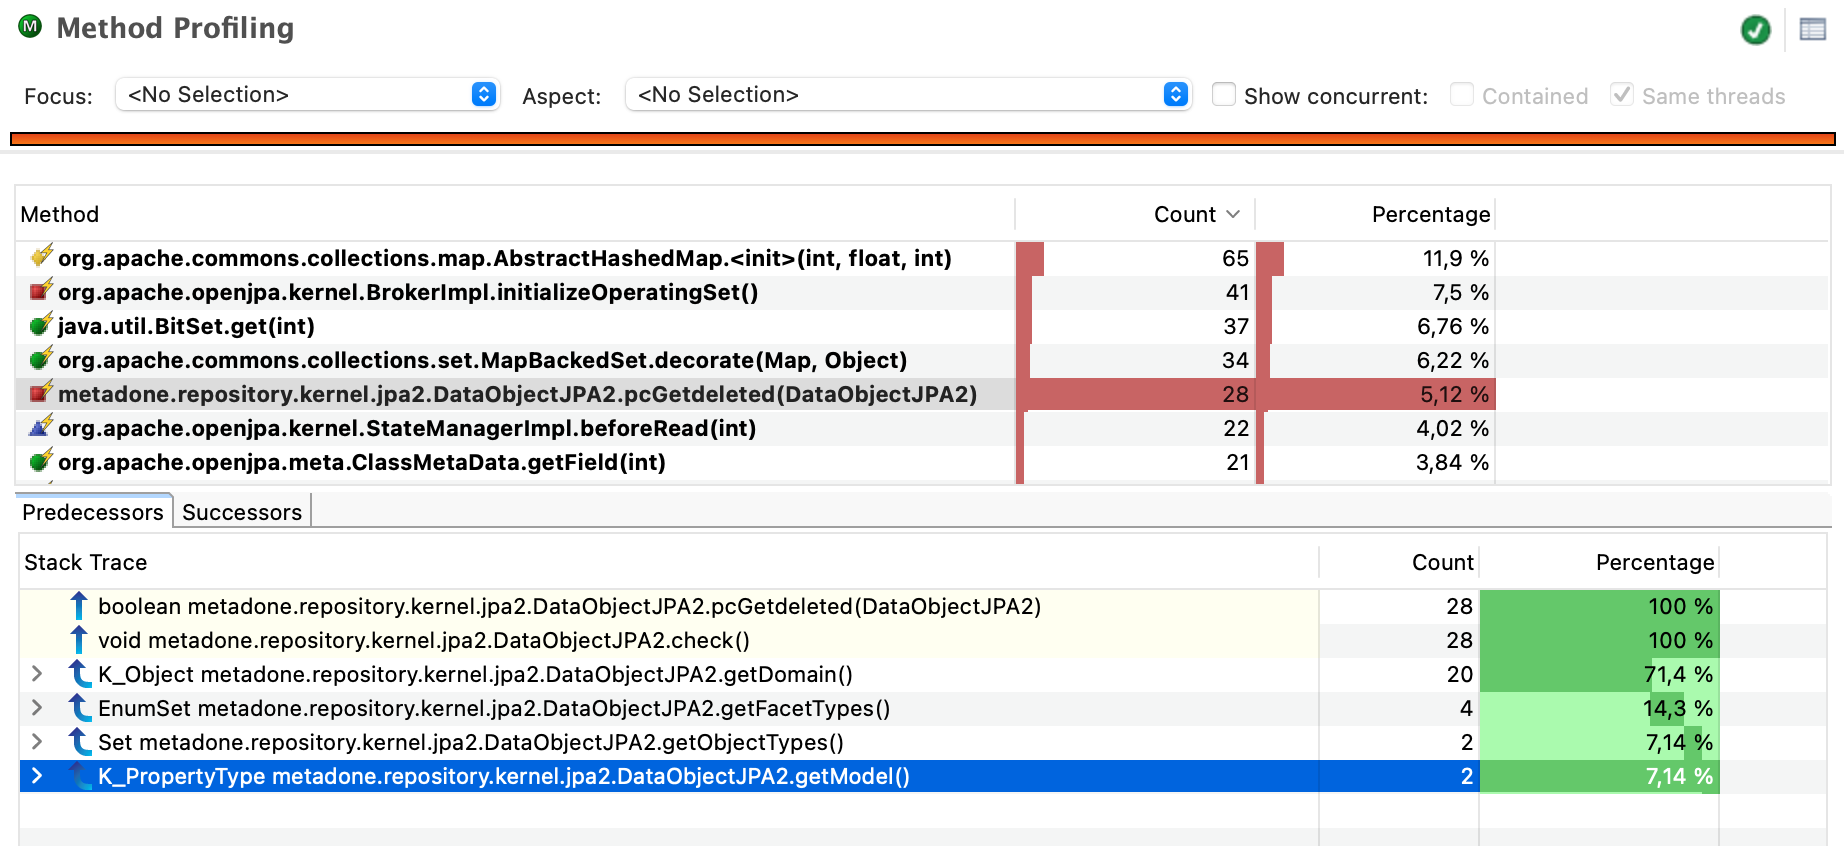
\includegraphics[width=0.9\textwidth]{img/scenario1/jfr-2.png}
\caption{Java Mission Control --- Method Profiling après optimisation.
Le compteur de la chaîne critique passe de 163 à 28 échantillons~;
\texttt{getModel} (bundle \texttt{metadone\_bundle\_repository\_jpa2})
tombe de 52,1\% à 7,14\% de charge CPU.}
\label{fig:jfr-2}
\end{figure}

% -----------------------------------------------
\subsubsection{Profilage post-optimisation avec async-profiler}
% -----------------------------------------------

Les flamegraphs de la figure~\ref{fig:prof2-zoom} isolent les mêmes
méthodes que celles analysées à la section~\ref{sec:scenario1-profil1},
permettant une comparaison directe avant/après.

\texttt{findMetaObjectsInDefinition\_oneshot}
(figure~\ref{fig:prof2-oneshot}) ne domine plus la pile d'appels~: sa
largeur dans le flamegraph est désormais négligeable, indiquant que les
traversées de \texttt{getRangeOf} dans le bundle
\texttt{metadone\_bundle\_repository} ont quasi disparu de la charge CPU
mesurée. Les opérations qui occupent maintenant le profil correspondent
à la construction légitime des objets du métamodèle, non plus à des
vérifications redondantes.

\begin{figure}[htbp]
\begin{subfigure}{\textwidth}
    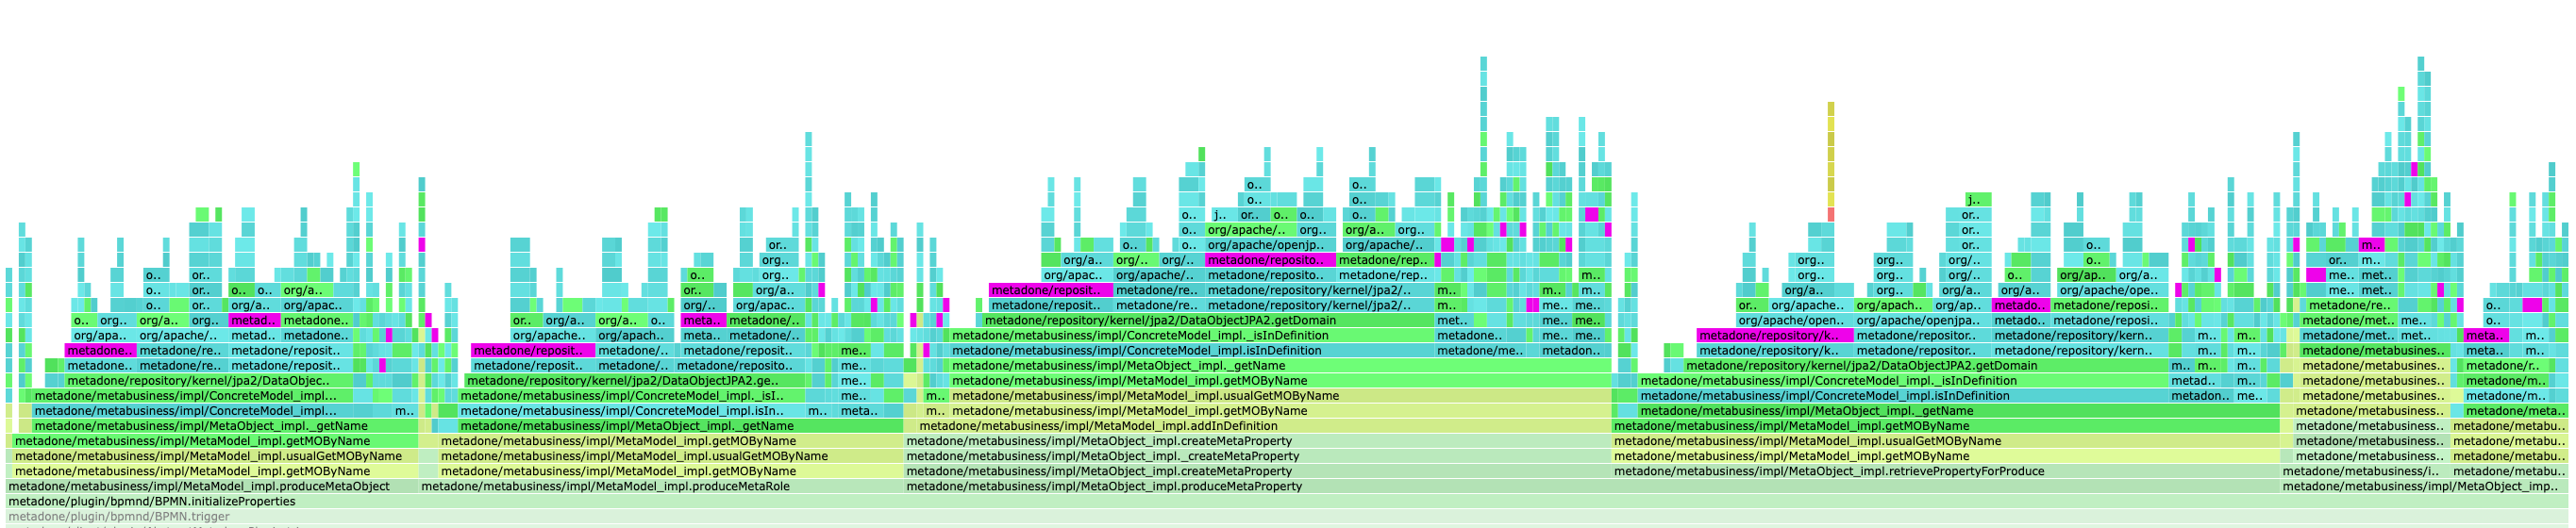
\includegraphics[width=\textwidth]{img/scenario1/prof2/pcGetdeleted.png}
    \caption{\texttt{pcGetdeleted} ---
    bundle \texttt{metadone\_bundle\_repository\_jpa2}}
    \label{fig:prof2-pcGetdeleted}
\end{subfigure}

\medskip
\begin{subfigure}{\textwidth}
    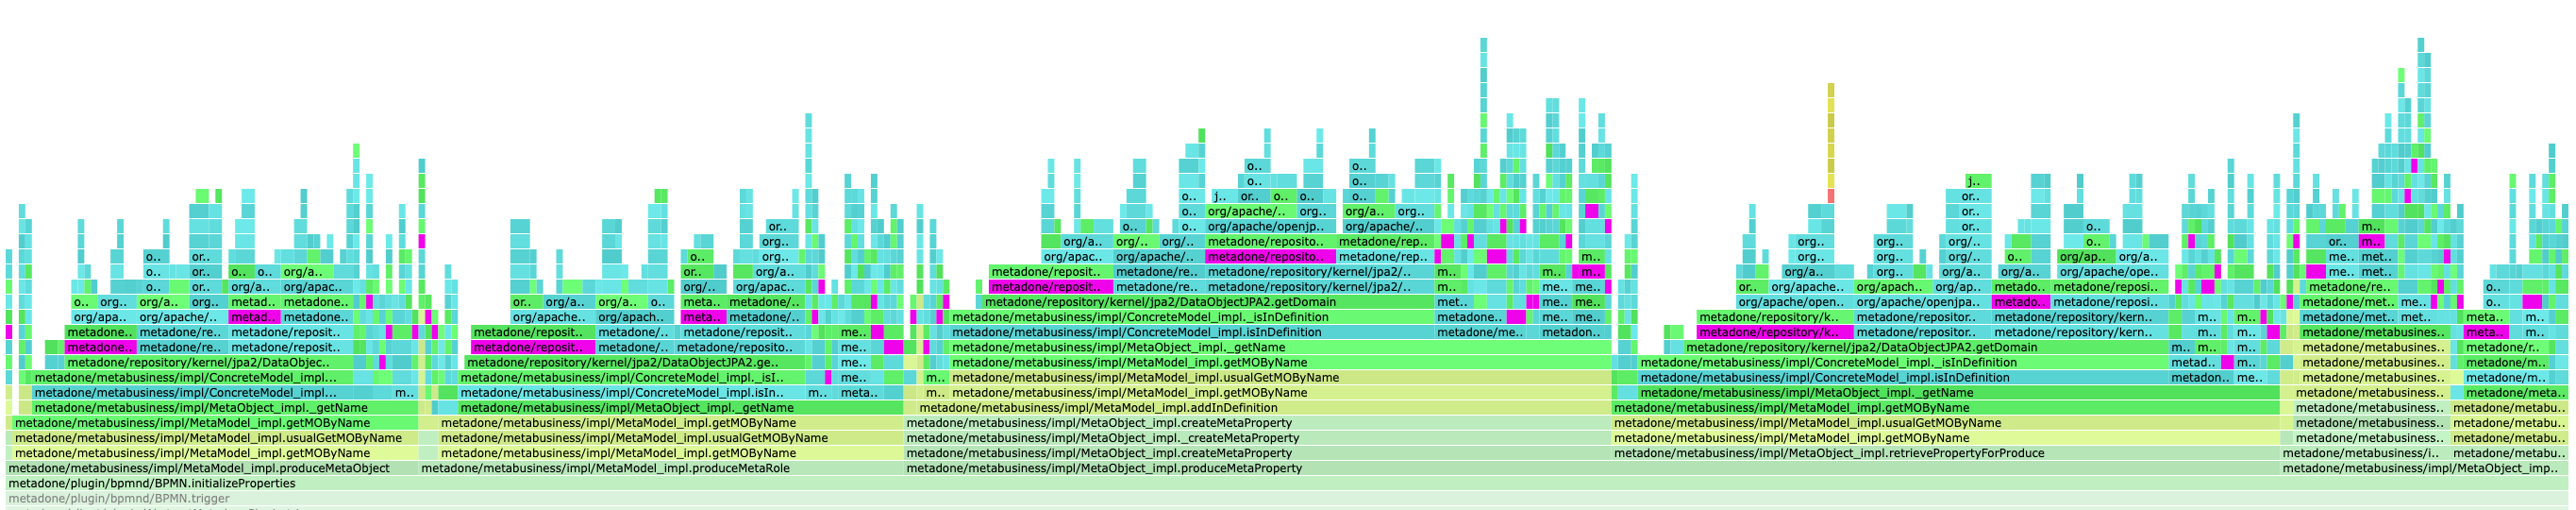
\includegraphics[width=\textwidth]{img/scenario1/prof2/check.png}
    \caption{\texttt{check} ---
    bundle \texttt{metadone\_bundle\_repository\_jpa2}}
    \label{fig:prof2-check}
\end{subfigure}

\medskip
\begin{subfigure}{\textwidth}
    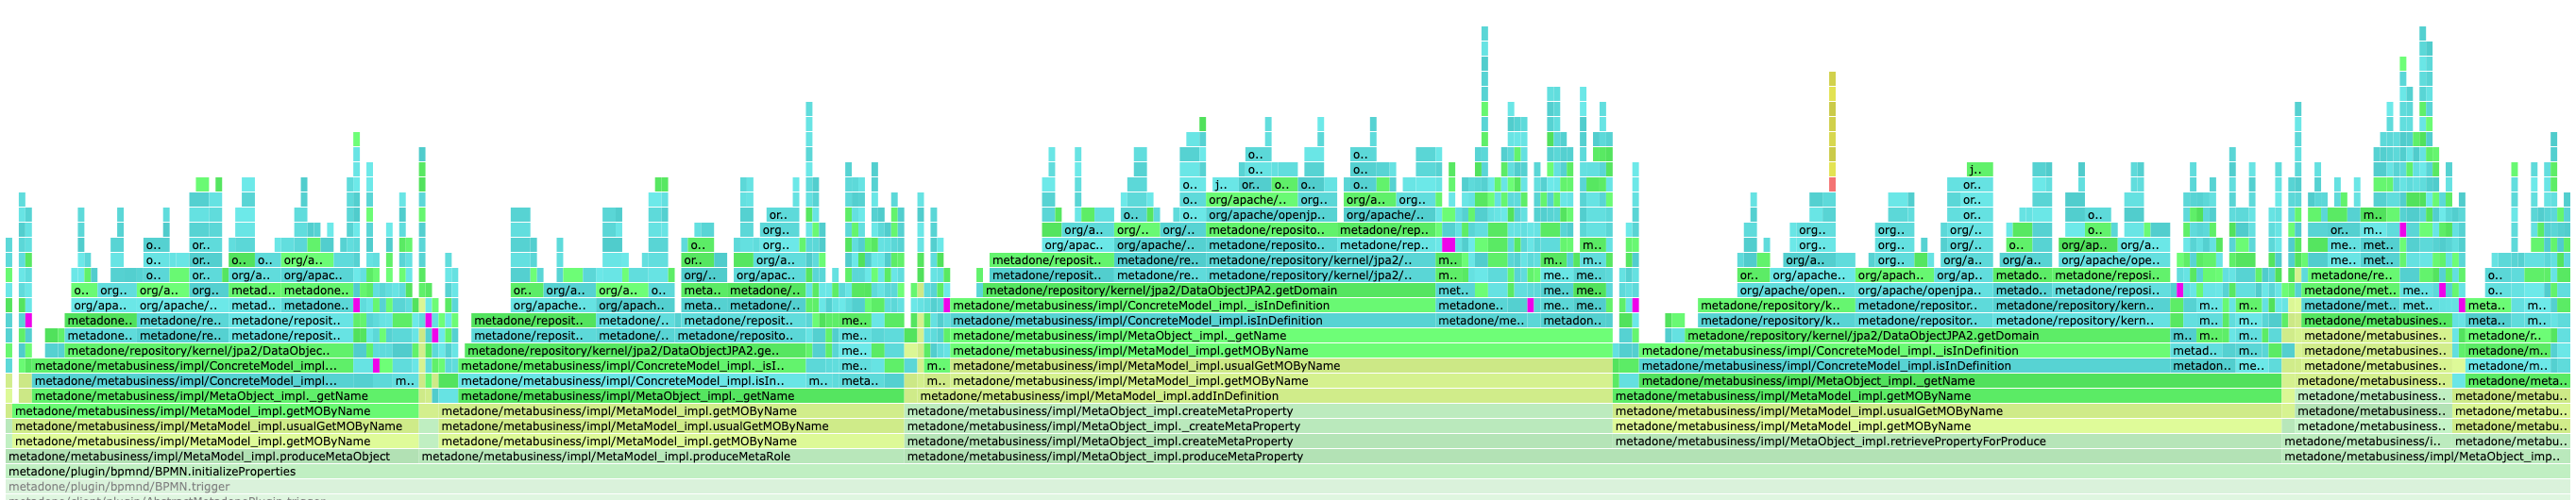
\includegraphics[width=\textwidth]{img/scenario1/prof2/getModel.png}
    \caption{\texttt{getModel} ---
    bundle \texttt{metadone\_bundle\_repository\_jpa2}}
    \label{fig:prof2-getModel}
\end{subfigure}

\medskip
\begin{subfigure}{\textwidth}
    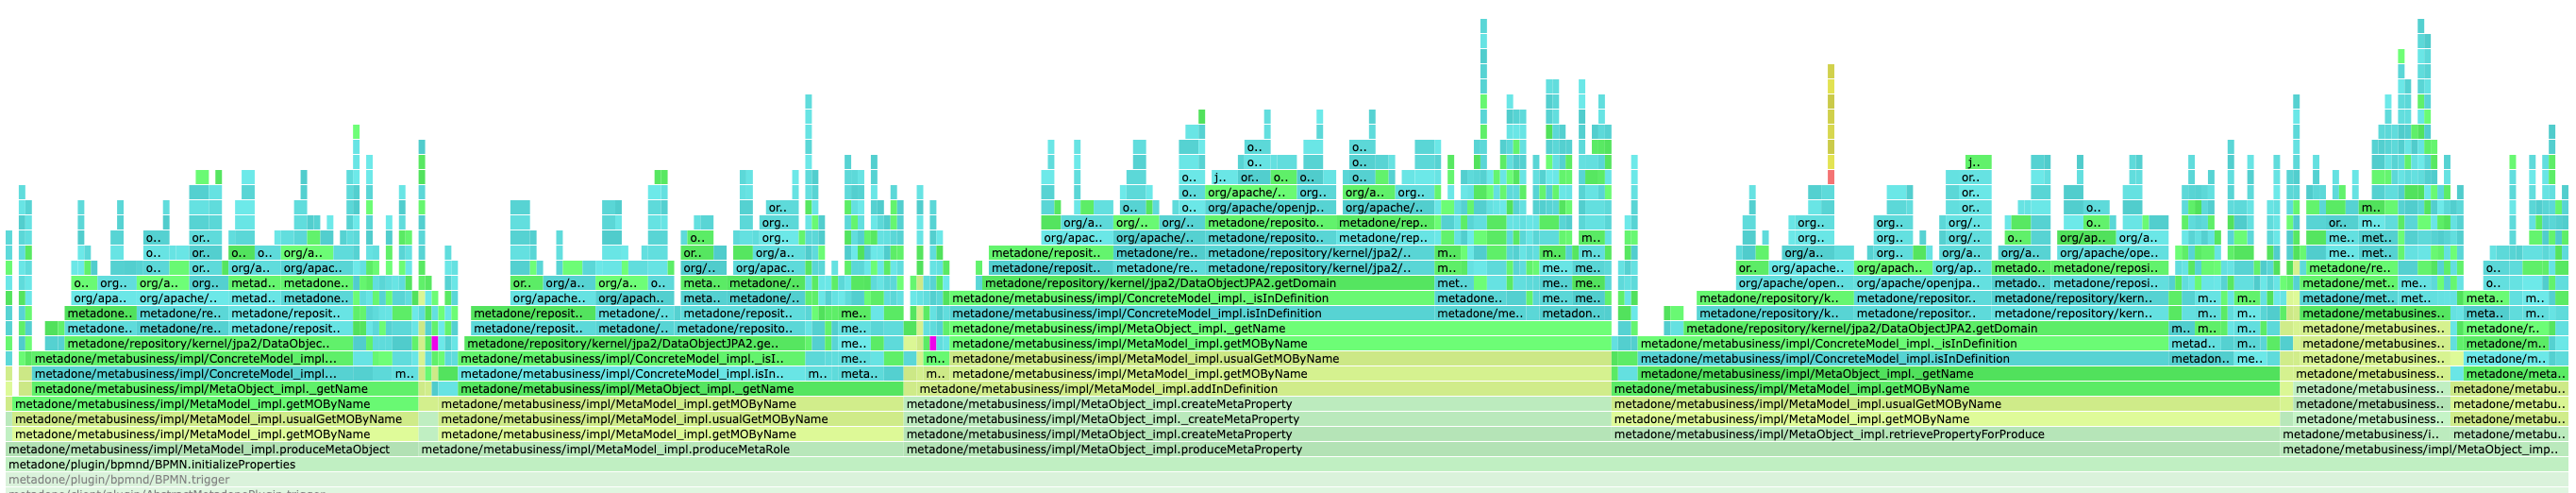
\includegraphics[width=\textwidth]{img/scenario1/prof2/getRangeOf.png}
    \caption{\texttt{getRangeOf} --- interface \texttt{K\_Object},
    bundle \texttt{metadone\_bundle\_repository}
    }
    \label{fig:prof2-getRangeOf}
\end{subfigure}

\medskip
\begin{subfigure}{\textwidth}
    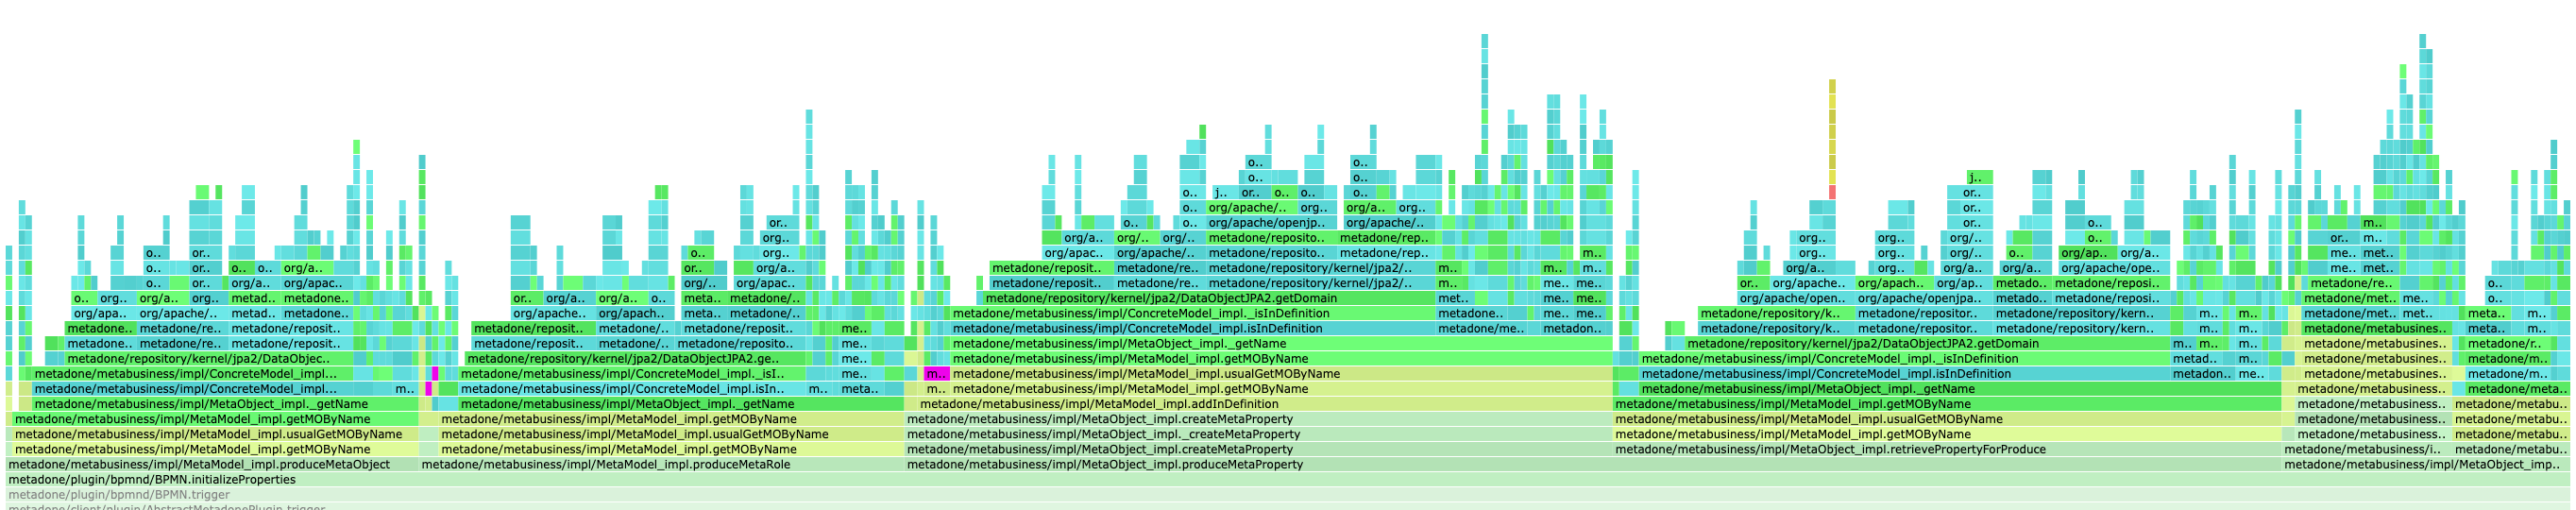
\includegraphics[width=\textwidth]{img/scenario1/prof2/oneshot.png}
    \caption{\texttt{findMetaObjectsInDefinition\_oneshot} ---
    classe \texttt{MetaModel\_impl},
    bundle \texttt{metadone\_bundle\_metabusiness}
    }
    \label{fig:prof2-oneshot}
\end{subfigure}

\caption{Flamegraphs post-optimisation --- même périmètre que la
figure~\ref{fig:prof1-zoom}. L'occupation CPU de
\texttt{findMetaObjectsInDefinition\_oneshot} et de la chaîne
\texttt{getRangeOf} $\to$ \texttt{getModel} $\to$ \texttt{check} $\to$
\texttt{pcGetdeleted} est désormais négligeable.}
\label{fig:prof2-zoom}
\end{figure}

% -----------------------------------------------
\subsubsection{Bilan du premier cycle d'optimisation}
% -----------------------------------------------

Le tableau~\ref{tab:bilan-opti1} synthétise les gains mesurés à l'issue
de ce premier cycle.

\begin{table}[h]
\centering
\caption{Bilan du premier cycle d'optimisation --- scénario
d'initialisation. Les médianes sont calculées sur 10 répétitions avec un
coefficient de variation inférieur à 1\,\% (mesures complètes en
annexe~\ref{ann:mesures-s1-a}).}
\label{tab:bilan-opti1}
\begin{tabular}{lrr}
\hline
\textbf{Indicateur} & \textbf{Baseline} & \textbf{Après opti.~1--3} \\
\hline
Temps de démarrage (médiane) & 18\,198~ms & 4\,516~ms \\
Facteur de réduction & --- & $\times$\,4,0 \\
Appels \texttt{findMetaObjectsInDefinition\_oneshot} & $\sim$80\,000 &
$\sim$750 \\
Charge CPU \texttt{getModel} (JFR) & 52,1\,\% & 7,14\,\% \\
Complexité algorithmique (dimension appartenance) & $O(n^2 \cdot s)$ & $O(n^2)$
\\
\hline
\end{tabular}
\end{table}

Au-delà du gain brut d'un facteur~4,0, ces modifications transforment
la \textbf{courbe de scalabilité} de MetaDONE. La version initiale
présentait une croissance en $O(n^2 \cdot s)$ du temps de bootstrapping
(cubique dans le pire cas où la hiérarchie de supertypes est profonde,
$s = O(n)$)~; la version optimisée ramène cette croissance à $O(n^2)$.
Cette différence est qualitative~: pour un métamodèle deux fois plus
grand, le coût ne croît plus selon la profondeur de la hiérarchie de
supertypes, rendant l'outil viable sur des modèles de grande envergure
là où l'architecture initiale l'aurait rendu impraticable.

Un goulot d'étranglement résiduel demeure néanmoins visible dans les
flamegraphs~: \texttt{pcGetdeleted} et \texttt{getRangeOf} conservent
une présence non négligeable dans la pile CPU, indiquant que les accès
au dépôt JPA restent coûteux indépendamment du cache applicatif. Ce
point constitue la piste d'investigation du prochain cycle d'analyse.
\subsection{Identification des goulots d'étranglement --- itération~2}
\label{sec:scenario1-profil2}

Après application des trois premières optimisations, une seconde session
de profilage a été conduite selon le même protocole que la
section~\ref{sec:scenario1-profil1}. Les figures~\ref{fig:jfr-2}
et~\ref{fig:prof2-zoom} avaient déjà confirmé l'efficacité des
corrections précédentes~: \texttt{findMetaObjectsInDefinition\_oneshot}
n'apparaît plus de manière dominante dans le profil CPU. Un nouveau
goulot d'étranglement émerge cependant, centré cette fois sur
\texttt{\_isInDefinition} et ses appels à \texttt{getDomain}.

% -----------------------------------------------
\subsubsection{Profilage CPU}
% -----------------------------------------------

En se concentrant sur les méthodes les plus représentées dans le
flamegraph post-optimisation~1--3, on obtient les pourcentages d'occupation
CPU suivants lors du bootstrapping~:

\begin{itemize}
    \item \texttt{pcGetdeleted} --- 21,33\%
    \item \texttt{check} --- 26,51\%
    \item \texttt{getDomain} --- 37,59\%
    \item \texttt{\_isInDefinition} / \texttt{isInDefinition} --- 37,23\%
    \item \texttt{\_getName} --- 48,43\%
    \item \texttt{getMOByName} --- 50,48\%
\end{itemize}

\texttt{getDomain} et \texttt{\_isInDefinition} apparaissent au même
niveau de profondeur dans le flamegraph, ce qui indique que
\texttt{getDomain} est appelé massivement \textit{depuis}
\texttt{\_isInDefinition}. La nouvelle chaîne d'appels critique est~:
\begin{center}
\small
\texttt{getMOByName} \\
$\downarrow$ \\
\texttt{\_getName}
(\texttt{MetaObject\_impl},
\texttt{metadone\_bundle\_metabusiness}) \\
$\downarrow$ \\
\texttt{isInDefinition} $\to$ \texttt{\_isInDefinition} 
(\texttt{ConcreteModel\_impl},
\texttt{metadone\_bundle\_metabusiness}) \\
$\downarrow$ \\
\texttt{getDomain} 
(interface \texttt{K\_Property},
\texttt{metadone\_bundle\_repository})
\end{center}

Notons que \texttt{getMOByName} et \texttt{\_getName} occupent toujours
le haut du profil (48--50\%) non plus à cause de la précondition
éliminée par l'optimisation~2, mais à cause du volume d'appels légitime
qu'ils génèrent vers \texttt{isInDefinition}. Le goulot a donc migré
d'un niveau vers le bas dans la pile d'appels.

% -----------------------------------------------
\subsubsection{Analyse statique et quantification}
% -----------------------------------------------

%\paragraph{Rôle de \texttt{\_isInDefinition}.}
La méthode \texttt{\_isInDefinition} est définie dans
\texttt{ConcreteModel\_impl} du bundle
\texttt{metadone\_bundle\_metabusiness}. Elle répond à une question
symétrique de \texttt{findMetaObjectsInDefinition\_oneshot}~: un
\texttt{ConcreteObject} donné appartient-il à la définition de ce
\texttt{ConcreteModel}~?

Pour le comprendre, il faut rappeler comment l'appartenance d'un objet
concret à un modèle est encodée dans le kernel: de même qu'un \texttt{MetaDef} relie un
\texttt{MetaObject} à son \texttt{MetaModel} via une \texttt{K\_Property}
de type \texttt{def\_pt}, un \texttt{ConcreteDef} relie un
\texttt{ConcreteObject} à son \texttt{ConcreteModel} par la même
structure. La méthode itère donc sur l'ensemble des \texttt{K\_Property}
dont \texttt{this} est le range via \texttt{getTarget().getRangeOf()}, et
pour chaque candidat, vérifie deux conditions~: que son domaine est bien
l'objet recherché (\texttt{candidate.getDomain() == kmember}), et que son
type de propriété est \texttt{def\_pt} (\texttt{someParentIsDef}).
Il s'agit d'une \textbf{recherche linéaire $O(n)$}, où $n$ est le nombre
de propriétés dont le \texttt{ConcreteModel} est le range.

\begin{lstlisting}[
  caption={\texttt{\_isInDefinition} --- classe \texttt{ConcreteModel\_impl},
  bundle \texttt{metadone\_bundle\_metabusiness}. Recherche linéaire $O(n)$
  sur les \texttt{K\_Property} du range~: chaque itération appelle
  \texttt{getDomain()} (interface \texttt{K\_Property},
  bundle \texttt{metadone\_bundle\_repository}).},
  label={ls-isinDefinition}]
private boolean _isInDefinition(ConcreteObject_impl member) {
    try {
        final K_Object kmember = member.getTarget();
        for (final K_Property candidate :
                getTarget().getRangeOf()) {
            if (candidate.getDomain() == kmember
                    && someParentIsDef(candidate)) {
                return true;
            }
        }
        return false;
    } catch (final BadFacet e) {
        throw new Metal2Exception(e);
    } catch (final BadPreCondition e) {
        throw new Metal2Exception(e);
    }
}
\end{lstlisting}

%\paragraph{Source de l'amplification.}
Rappelons que \texttt{\_getName} (section~\ref{sec:opti-metamodel},
optimisation~2) parcourt les \texttt{ConcreteProperty<String>} associées
au \texttt{MetaObject} et appelle \texttt{concreteModel.isInDefinition(cp)}
pour chacune afin de déterminer si la propriété de nom appartient au bon
\texttt{ConcreteModel} (Listing~\ref{ls--getname}, ligne~378). Chaque
appel à \texttt{isInDefinition} déclenche un scan complet via
\texttt{\_isInDefinition}. Si la propriété n'est pas trouvée dans le
\texttt{MetaModel} courant, \texttt{\_getName} remonte récursivement dans
ses supertypes directs (ligne~383), multipliant encore le nombre d'appels.

L'instrumentation confirme cette amplification~: pour
\textbf{1~700~appels} à \texttt{\_getName}, on dénombre plus de
\textbf{74~000~appels} à \texttt{\_isInDefinition}, soit un
\textbf{facteur multiplicatif moyen de 43}. Ce ratio est du même ordre
que le facteur~57 observé à la section~\ref{sec:scenario1-profil1}~: la
structure du problème est identique --- une boucle externe génère une
amplification quadratique via une recherche linéaire interne --- mais le
point d'application s'est déplacé d'un niveau vers le bas dans la pile
d'appels, de \texttt{MetaModel\_impl} vers \texttt{ConcreteModel\_impl}.

%\paragraph{Parallèle avec le problème précédent.}
Le schéma identifié ici est la réplique exacte de celui de
l'itération~1 (section~\ref{sec:scenario1-profil1}), mais opérant
cette fois sur le niveau concret (M1) de MetaL$_2$ plutôt que sur
son niveau méta-modèle (M2/M3)~:

\begin{center}
\small
\begin{tabular}{lll}
\hline
\textbf{Dimension} & \textbf{Itération~1} & \textbf{Itération~2} \\
\hline
Niveau (dans MetaL$_2$) & Méta-modèle (M2/M3) & Concret (M1) \\
Classe & \texttt{MetaModel\_impl} & \texttt{ConcreteModel\_impl} \\
Méthode centrale & \texttt{\_hasInItsDefinition} &
\texttt{\_isInDefinition} \\
Scan interne & \texttt{findMetaObjectsInDefinition\_oneshot} &
\texttt{\_isInDefinition} elle-même \\
Opération de base & \texttt{getRangeOf(def\_pt)} & \texttt{getRangeOf()} \\
Facteur d'amplification & $\sim$57 & $\sim$43 \\
\hline
\end{tabular}
\end{center}

Cette récurrence est la conséquence directe de la symétrie réflexive
entre les niveaux méta et concret de MetaL$_2$, documentée à la
section~\ref{sec:reflexivite-intro}~: \texttt{MetaModel} et
\texttt{ConcreteModel} reposent tous deux sur le substrat uniforme
de \texttt{DataObject} (MetaL$_1$, bundle \texttt{repository}) et
encodent l'appartenance de la même manière. Les algorithmes qui la
vérifient partagent donc la même structure et les mêmes
vulnérabilités. La solution sera également symétrique~: l'introduction
d'un cache dans \texttt{ConcreteModel\_impl}, à l'image de ce qui a
été fait dans \texttt{MetaModel\_impl}.

% -----------------------------------------------
\subsubsection{Synthèse du diagnostic}
% -----------------------------------------------

Le goulot résiduel identifié après la première itération d'optimisation est
analogue à celui de l'itération~1, mais opère au niveau concret (M1) de
MetaL$_2$.
La pile d'appels problématique est~:

\begin{center}
\small
\texttt{ConcreteModel\_impl.\_isInDefinition} \\
(itération $O(n)$ sur toutes les \texttt{K\_Property} du range) \\[4pt]
$\downarrow$ \\[4pt]
\texttt{K\_Property.getDomain} ---
\texttt{metadone\_bundle\_repository} \\
(accès au dépôt JPA à chaque itération)
\end{center}

La mitigation naturelle est identique à celle de l'itération~1~: la
mémoïsation des résultats via un cache. Dans
\texttt{ConcreteModel\_impl}, l'appartenance d'un
\texttt{ConcreteObject} à un \texttt{ConcreteModel} est une information
qui change rarement une fois le modèle construit~; elle est un candidat
idéal pour la mise en cache. La phase d'optimisation suivante développe
cette stratégie.

\subsection{Optimisation --- itération~2}
\label{sec:scenario1-opti2}

\subsubsection{Optimisation~4 : cache d'appartenance dans
\texttt{ConcreteModel\_impl}}
\label{sec:opti4}

%\paragraph{Principe.}
Le diagnostic de la section~\ref{sec:scenario1-profil2} a mis en évidence
que \texttt{\_isInDefinition} était appelée 74~000 fois pour seulement
1~700~appels à \texttt{\_getName}, et que chaque appel déclenchait un scan
linéaire complet via \texttt{getRangeOf()} et \texttt{getDomain()} dans
le bundle \texttt{metadone\_bundle\_repository}. Le correctif introduit un cache
d'appartenance directement dans \texttt{ConcreteModel\_impl}
(\texttt{metadone\_bundle\_metabusiness}), afin que chaque paire
(\texttt{ConcreteModel}, \texttt{ConcreteObject}) ne soit scannée qu'une
seule fois.

Cette approche est la réplique exacte, au niveau concret (M1) de
MetaL$_2$, du mécanisme de \texttt{CacheCallFunction} utilisé dans
\texttt{MetaModel\_impl} pour \texttt{\_hasInItsDefinition}
(optimisations~1 et~3, section~\ref{sec:opti-metamodel}). La symétrie
réflexive entre les niveaux méta et concret de MetaL$_2$, documentée
à la section~\ref{sec:reflexivite-intro}, se retrouve ici dans la
solution autant que dans le problème.

%\paragraph{Structure du cache.}
Le cache est déclaré comme champ d'instance \texttt{private final} de
\texttt{ConcreteModel\_impl}~:

\begin{lstlisting}[firstnumber=42,
  caption={Déclaration du cache dans \texttt{ConcreteModel\_impl} ---
  bundle \texttt{metadone\_bundle\_metabusiness}.},
  label={ls-cache-isin}]
private final Map<ConcreteObject_impl, Boolean>
    cache_isInDefinition =
        new WeakHashMap<ConcreteObject_impl, Boolean>();
\end{lstlisting}

Le choix d'un \texttt{WeakHashMap} est délibéré et cohérent avec celui
fait pour le cache de proxies dans \texttt{FactoryOfProxy}~: les clés sont des références faibles vers
les \texttt{ConcreteObject\_impl}. Lorsqu'un objet n'est plus référencé
ailleurs dans la JVM, il peut être collecté par le ramasse-miettes sans
que le cache ne l'en empêche, et l'entrée correspondante disparaît
automatiquement. Cela évite toute fuite mémoire dans un système où les
objets concrets peuvent être supprimés à l'exécution via
\texttt{removeFromDefinition}.

Par ailleurs, le cache mémorise les \textbf{deux résultats possibles}
(\texttt{true} et \texttt{false})~: il évite ainsi de rescanner pour
des objets dont l'absence est déjà connue, ce qui est important dans les
appels de vérification défensifs effectués avant un ajout.

%\paragraph{Logique de consultation.}
La méthode \texttt{\_isInDefinition} réécrite est présentée au
Listing~\ref{ls-isinDefinition-cache}. Elle consulte désormais le
cache avant tout accès au repository~: en cas de succès
(\textit{cache hit}), la réponse est retournée en $O(1)$~; en cas
d'échec (\textit{cache miss}), le scan $O(n)$ est effectué et son
résultat --- positif ou négatif --- est mémorisé avant d'être
retourné.

\begin{lstlisting}[language=Java, firstnumber=141,
  caption={\texttt{\_isInDefinition} après l'optimisation~4 ---
  classe \texttt{ConcreteModel\_impl},
  bundle \texttt{metadone\_bundle\_metabusiness}. Le cache est
  consulté avant tout scan~; les deux résultats (positif et
  négatif) sont mémorisés.},
  label={ls-isinDefinition-cache}]
private boolean _isInDefinition(ConcreteObject_impl member) {
    try {
        // Check cache first
        Boolean cached = cache_isInDefinition.get(member);
        if (cached != null) {
            return cached;
        }

        // Cache miss: perform the scan
        final K_Object kmember = member.getTarget();
        for (final K_Property candidate : getTarget().getRangeOf()) {
            if (candidate.getDomain() == kmember
                    && someParentIsDef(candidate)) {
                cache_isInDefinition.put(member, true);
                return true;
            }
        }

        // Not found: store false and return
        cache_isInDefinition.put(member, false);
        return false;
    } catch (final BadFacet e) {
        throw new Metal2Exception(e);
    } catch (final BadPreCondition e) {
        throw new Metal2Exception(e);
    }
}
\end{lstlisting}

Notons que le gain de performance attendu ne porte pas sur le nombre
d'invocations de \texttt{\_isInDefinition} --- qui reste identique
puisque les call sites en amont (\texttt{\_getName} en particulier)
ne sont pas modifiés --- mais sur le \textbf{coût unitaire} de chaque
appel~: ce qui était auparavant un scan $O(n)$ du graphe devient,
dans la majorité des cas, un accès $O(1)$ à la \texttt{WeakHashMap}.
La mesure pertinente du gain est donc le temps mural, analysé à la
section~\ref{sec:scenario1-tests2}.

%\paragraph{Cohérence du cache lors des mutations.}
Deux méthodes modifient la définition d'un \texttt{ConcreteModel} et
doivent maintenir la cohérence du cache~:

\begin{itemize}
    \item \texttt{\_addInDefinition} insère directement \texttt{true}
    dans le cache après l'ajout. Cela évite qu'un appel immédiat à
    \texttt{\_isInDefinition} ne déclenche un scan inutile pour un objet
    dont on vient d'établir l'appartenance --- comportement analogue à la
    mise à jour incrémentale de l'optimisation~3
    (section~\ref{sec:opti-metamodel}).

    \item \texttt{removeFromDefinition} invalide l'entrée via
    \texttt{cache\_isInDefinition.remove(member)} après suppression. Au
    prochain appel, \texttt{\_isInDefinition} effectuera un scan et
    constatera l'absence, qu'elle mettra alors en cache avec
    \texttt{false}.
\end{itemize}

Le cache étant de portée instance, chaque \texttt{ConcreteModel\_impl}
maintient son propre état d'appartenance indépendamment des autres
modèles, ce qui est cohérent avec la sémantique de
\texttt{isInDefinition}~: un même \texttt{ConcreteObject} peut appartenir
à plusieurs \texttt{ConcreteModel} simultanément
(comportement par défaut lorsque la propriété
\texttt{canNotBeShared} de \texttt{MetaDef} n'est pas activée~;
cf.~section~\ref{sec:metal2}).

%\paragraph{Impact sur la complexité.}
Avant l'optimisation, chaque appel à \texttt{\_isInDefinition} coûtait
$O(n)$ où $n$ est le nombre de \texttt{K\_Property} dans le range du
\texttt{ConcreteModel}. Après l'optimisation, le coût est $O(1)$ pour
toute requête déjà vue, et $O(n)$ uniquement lors du premier scan pour
chaque paire (\texttt{ConcreteModel}, \texttt{ConcreteObject}). Dans le
contexte de \texttt{\_getName}, qui interroge les mêmes propriétés de
nom de manière répétitive lors du bootstrapping, le nombre de scans
effectifs tend vers $O(k)$ où $k$ est le nombre de paires distinctes
plutôt que vers $O(n \times \text{appels})$.

% -------------------------------------------------------------------
\subsection{Tests de performance --- itération~2}
\label{sec:scenario1-tests2}
% -------------------------------------------------------------------

\subsubsection{Bilan du second cycle d'optimisation}

Le tableau~\ref{tab:bilan-opti2} synthétise les gains cumulés à l'issue
des deux cycles d'optimisation.

\begin{table}[h]
\centering
\caption{Bilan cumulé des deux cycles d'optimisation ---
scénario d'initialisation. Les médianes sont calculées sur 10~répétitions
(mesures complètes en annexe~\ref{ann:mesures-s1-a}).}
\label{tab:bilan-opti2}
\begin{tabular}{lrrr}
\hline
\textbf{Indicateur} & \textbf{Baseline} & \textbf{Après~1--3} &
\textbf{Après~1--4} \\
\hline
Temps de démarrage (médiane, ms) & 18\,198 & 4\,516 & 1\,490 \\
Facteur cumulé & --- & $\times$\,4,0 & $\times$\,12,2 \\
Complexité (appartenance, niveau méta) & $O(n^2 \cdot s)$ & $O(n^2)$ & $O(n^2)$ \\
Complexité (appartenance, niveau concret) & $O(n^2)$ & $O(n^2)$ &
$O(n \cdot k)$ \\
\hline
\end{tabular}
\end{table}

Le passage de $\times$\,4,0 à $\times$\,12,2 illustre l'effet
multiplicateur d'une optimisation portant sur le coût unitaire dans une
boucle déjà serrée par les cycles précédents~: une fois la redondance
structurelle éliminée (iter.~1), même un cache à coût quasi-nul produit
un gain important.

% -------------------------------------------------------------------
\subsection{Synthèse du scénario~1}
\label{sec:scenario1-synthese}
% -------------------------------------------------------------------

Le scénario d'initialisation a permis d'identifier et de résoudre deux
familles de goulots d'étranglement successives, toutes deux enracinées
dans la même propriété architecturale de MetaDONE~: l'encodage uniforme
de l'appartenance et du typage dans un graphe homogène de
\texttt{DataObject}.

La première famille (optimisations~1--3) portait sur le niveau
méta-modèle (M2/M3) de MetaL$_2$~: le cache de \texttt{MetaModel\_impl}
était structurellement inopérant, transformant une vérification
d'appartenance $O(1)$ en un scan $O(n)$ répété, lui-même amplifié d'un
facteur~57 par la boucle de \texttt{getMOByName}. La complexité
effective du bootstrapping était $O(n^3)$.

La seconde famille (optimisation~4) portait sur le niveau concret
(M1) de MetaL$_2$~: la symétrie réflexive entre les deux niveaux
s'est retrouvée dans le problème lui-même.
\texttt{\_isInDefinition} dans \texttt{ConcreteModel\_impl}
reproduisait exactement le même antipattern, avec un facteur
d'amplification de~43.

Ces deux familles partagent une cause commune~: l'absence de mémoïsation
sur des résultats stables. Les \texttt{DataObject} d'un projet MetaDONE
sont majoritairement en lecture une fois le bootstrapping achevé~; le
coût de maintien des caches (invalidation sur mutation, mise à jour
incrémentale sur ajout) est donc faible comparé au gain sur les accès.
Cette observation est cohérente avec les recommandations générales de la
littérature sur les applications à forte intensité de lecture sur des
graphes~\cite{oaks2014java, fowler2002patterns}.

Les quatre optimisations sont ciblées, non invasives et n'affectent
pas les contrats publics des interfaces de MetaL$_2$ (aux deux
niveaux méta et concret)~: elles opèrent exclusivement dans les
classes \texttt{*\_impl} du bundle \texttt{metadone\_bundle\_metabusiness},
sans modifier le bundle \texttt{repository} qui implémente MetaL$_1$,
ni les interfaces exposées aux plugins.

\paragraph{Confrontation à l'hypothèse initiale.}
L'hypothèse formulée en méthodologie (section~\ref{sec:scenarios})
selon laquelle cette phase d'initialisation souffrirait du problème
du N+1 et des limites du \emph{lazy loading} n'a pas été validée par
les mesures~: les goulots identifiés (familles~1 et~2 ci-dessus) sont
strictement CPU-bound et algorithmiques. Aucune des chaînes d'appels
critiques ne déclenche d'accès supplémentaires à la base de données
au-delà du chargement initial~; les boucles linéaires problématiques
opèrent toutes sur des collections JPA déjà chargées dans l'identity
map. Le surcoût JPA effectif, mesurable mais minoritaire après
optimisations (\texttt{pcGetdeleted} et \texttt{getRangeOf} ci-dessous),
n'affecte pas la conclusion principale.

\paragraph{Limites et goulots résiduels.}
\texttt{pcGetdeleted} et \texttt{getRangeOf} conservent une présence
non négligeable dans les profils post-optimisation. Ces méthodes
appartiennent au bundle \texttt{metadone\_bundle\_repository\_jpa2} et
reflètent le coût intrinsèque des accès à la base de données via OpenJPA,
indépendamment des caches applicatifs. Leur réduction nécessiterait
d'agir à un niveau différent~: stratégie de chargement JPA (batch
fetching, eager vs. lazy), indexation de la colonne \texttt{range} dans
le schéma relationnel, ou remplacement partiel des requêtes par des
structures en mémoire. Ces pistes constituent les axes d'investigation
des scénarios suivants.

\newpage
\section{Scénario 2 : Chargement d'un script GraSyLa}
\label{sec:scenario2}

\subsection{Description et enjeux}
Ce scénario mesure les performances de chargement d'un script GraSyLa dans MetaDONE. Le script retenu pour les mesures est bpmn\_mm.grasyla, le méta-modèle BPMN fourni avec le plugin BPMN de MetaDONE. Il contient 106 équations et constitue un cas représentatif d'un script de taille réelle.

Le processus de chargement a été décomposé en quatre phases mesurées indépendamment, synthétisées au tableau~\ref{tab:scenario2-phases}~:

\begin{table}[h]
\centering
\caption{Phases du scénario 2}
\label{tab:scenario2-phases}
% On définit la largeur totale (\textwidth) et on utilise "X" pour la colonne étirable
\begin{tabularx}{\textwidth}{lXl}
\hline
\textbf{Phase} & \textbf{Description} & \textbf{Temps (ms)} \\
\hline
t1 - Parsing & Transformation du texte source en AST par ANTLR & $\sim$ 18\\
t2 - Génération (création) & Matérialisation de l'AST en objets MetaL$_2$ persistés (première création) & $\sim$ 4\,100\\
t3 - Génération (mise à jour) & Re-génération du même script déjà présent en base & $\sim$ 1~700\\
t4 - Traversée & Lecture des équations et imports depuis la base & $\sim$ 2\\
\hline
\end{tabularx}
\end{table}
Les mesures de référence du Scénario 2 ont été collectées sur le code après application des optimisations du Scénario 1, afin de refléter l'état incrémental du logiciel à ce stade du cycle d'optimisation. Elles ont par ailleurs été obtenues sans assertions Java actives (option \texttt{-ea} désactivée), afin d'isoler le comportement de la couche applicative du coût des vérifications internes liées au \emph{Design by Contract} (section~\ref{sec:dbc}).

La phase de parsing (t1) est négligeable. La phase de traversée (t4) est quasi-instantanée, ce qui confirme que le cache JPA fonctionne correctement en lecture. La phase de création (t2) est en revanche 228 fois plus lente que le parsing, ce qui localise sans ambiguïté le problème du côté de la persistance JPA lors de la génération.

L'écart entre t2 et t3 (\textasciitilde 4\,100~ms contre \textasciitilde 1\,700~ms pour la même charge) mérite d'être souligné~: la re-génération d'un script déjà présent en base est environ 2,4 fois plus rapide que sa création initiale. Lors de la re-génération, les objets \texttt{K\_Object} et \texttt{K\_Property} correspondant aux équations existent déjà dans l'identity map JPA~; le coût se réduit à des vérifications de cohérence et à la mise à jour de quelques attributs, sans déclencher l'avalanche d'insertions caractéristique de la première création. Cette asymétrie confirme que le goulot d'étranglement se situe précisément dans les opérations d'insertion JPA et non dans la logique de traversée de l'AST.

\subsection{Identification du goulot d'étranglement}
Un profil d'exécution a été collecté à l'aide d'async-profiler sur la phase t2 (voir figure \ref{fig:async-createRole}). Les fonctions principales identifiées et leur pourcentage CPU sont les suivantes:
\begin{itemize}
    \item ConcreteModel\_impl.\_createRole(): 72\%
    \item AST\_expression.generate(): 76\%
\end{itemize}
\begin{figure}[h]
\centering
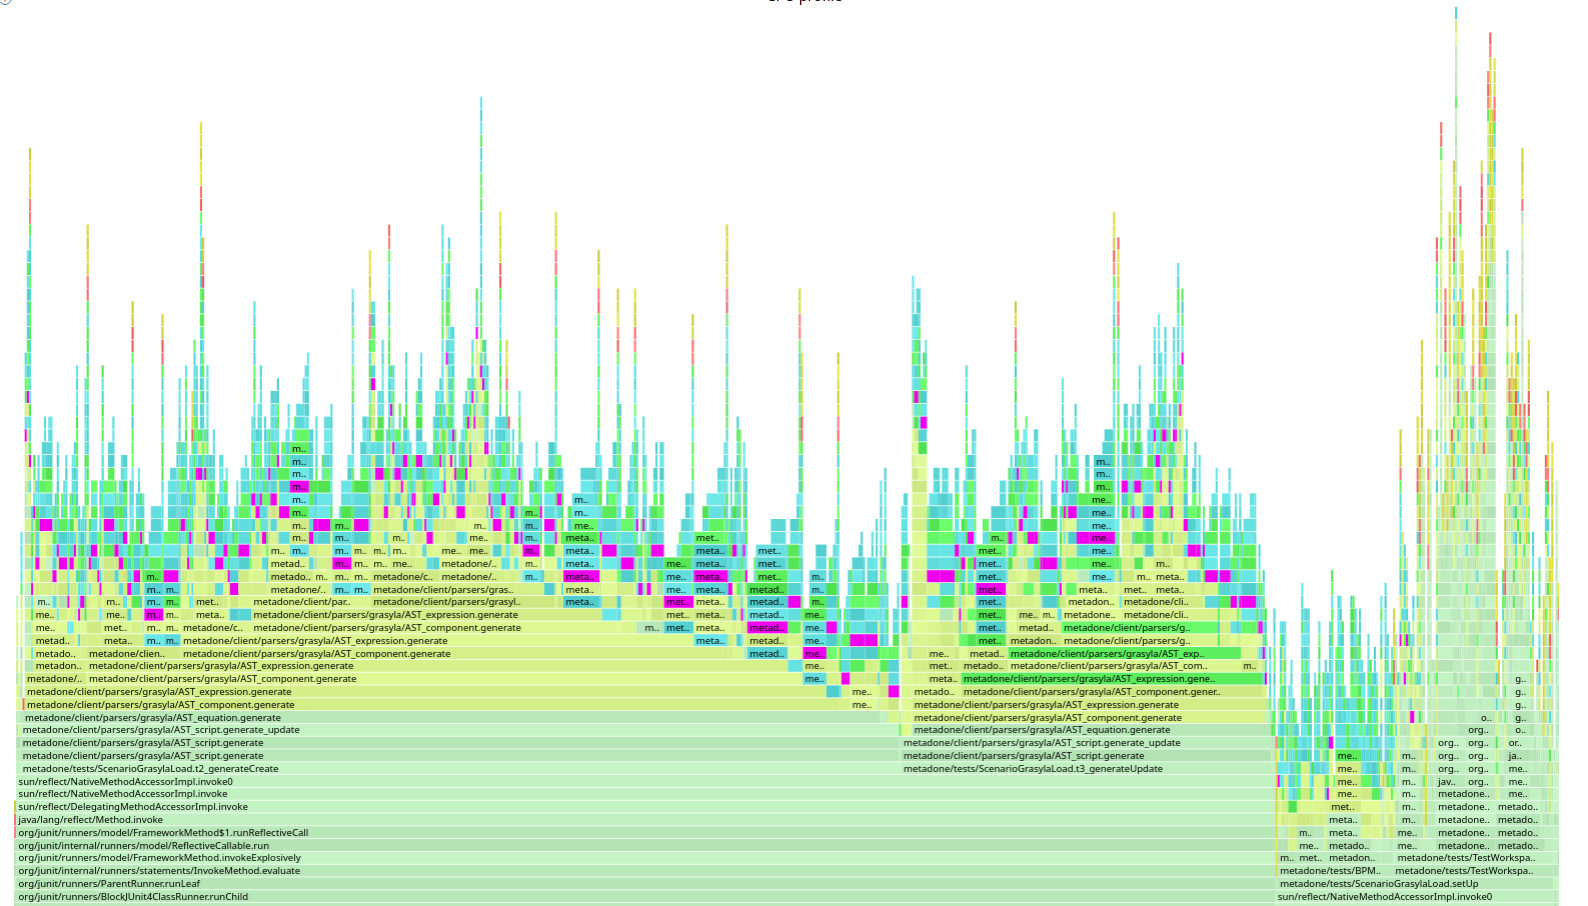
\includegraphics[width=0.9\textwidth]{img/createRole.png}
\caption{Flamegraph avec la fonction \texttt{ConcreteModel\_impl.\_createRole()} (bundle \texttt{metadone\_bundle\_metabusiness}) mise en évidence}
\label{fig:async-createRole}
\end{figure}
Le fait que \texttt{\_createRole()} représente 72\,\% du temps total, et que cette méthode soit appelée exclusivement depuis \texttt{AST\_expression.generate()} (76\,\%), indique que la quasi-totalité du temps de génération est consommée par les opérations d'écriture JPA, et non par la logique de traversée de l'AST ni par les vérifications de précondition.

À titre de comparaison, la méthode \texttt{getDefinitionRestricted()}, annotée du commentaire \texttt{// XXX horrible performance} dans le code source, ne représente que 0,14\,\% du temps d'exécution. Ce contraste illustre concrètement la nécessité de mesurer avant d'optimiser~: la fonction signalée comme problématique s'avère négligeable, tandis que le véritable goulot se situe ailleurs.

\subsection{Analyse du goulot : la persistance du ConcreteRole}
Le modèle de données de MetaDONE repose sur le méta-modèle MetaL$_2$, dans lequel tout est un objet, y compris les rôles concrets. Un \texttt{ConcreteRole} n'est pas un simple lien entre deux objets ; c'est lui-même une entité de premier rang, dotée d'une identité propre et susceptible de porter des propriétés ou d'être lui-même domaine ou range d'un autre rôle.

Cette décision architecturale se traduit directement dans la couche de persistance JPA. Chaque appel à \texttt{\_createRole()} exécute deux opérations d'insertion distinctes~:
\begin{lstlisting}[firstnumber=332,
  caption={Création du rôle avec \texttt{K\_Object} et \texttt{K\_Property} ---
  méthode \texttt{ConcreteModel\_impl.\_createRole()},
  bundle \texttt{metadone\_bundle\_metabusiness}.},
  label={ls-createRole}]
try {
    final K_PropertyType theMetaRole = mr.getMetaroleType();

    final K_Object result_o = mr.getTarget().createObject(); // INSERT #1 : K_Object
    theMetaRole.createProperty(result_o.getDataObject(), domain.getTarget(), range.getTarget()); // INSERT #2 : K_Property
    final ConcreteRole_impl result = FactoryOfProxy.buildConcreteRole(result_o);
    this.addInDefinition(result);
    return result;
}
\end{lstlisting}

\texttt{K\_Object} représente le \texttt{ConcreteRole} comme entité autonome dans la base. Il reçoit un identifiant unique (OID) et est stocké dans la table des objets. \texttt{K\_Property} représente le lien typé entre le domaine, le range et le \texttt{K\_PropertyType} correspondant au \texttt{MetaRole} qui gouverne ce lien.
Dans un modèle relationnel classique, un lien entre deux objets se réduirait à une ligne dans une table de jointure --- un seul INSERT. La généralité de MetaL$_2$ exige ici deux entités JPA par rôle, doublant mécaniquement le nombre d'opérations d'écriture. Pour un script de 106 équations dont chacune contient un arbre d'expressions potentiellement profond, ce surcoût se répercute sur des centaines à des milliers d'insertions lors d'une seule opération de chargement.

\subsection{Optimisations étudiées}
\label{sec:scenario2-opti}

Le goulot étant dans les INSERTs JPA eux-mêmes, toute amélioration significative devra agir à ce niveau. Une candidate locale a d'abord été examinée puis écartée~; trois pistes plus structurelles sont ensuite discutées.

\subsubsection{Court-circuit de la précondition (écartée)}
\label{sec:scenario2-precondition-rejet}

La méthode \texttt{precondition\_createRole()} vérifie, avant chaque création de rôle, que la cardinalité du \texttt{MetaRole} n'est pas violée. Pour la cardinalité \texttt{MANY\_TO\_MANY} --- utilisée notamment par les rôles liant chaque expression à ses éléments enfants --- la vérification consiste à parcourir l'ensemble des propriétés existantes depuis le domaine pour détecter d'éventuels doublons. Cette traversée est de complexité $O(N)$ par appel, soit $O(N^2)$ au total pour $N$ enfants d'un même nœud.

Cependant, le profileur positionne la précondition à moins de 1\,\% du temps d'exécution total. Deux facteurs expliquent ce résultat~: les collections JPA sont maintenues en mémoire dans l'identity map (la traversée est une itération Java pure, sans accès base), et le nombre d'enfants par nœud d'expression reste structurellement limité dans les scripts réels.

Au-delà du gain nul attendu, court-circuiter la précondition violerait le principe de \emph{Design by Contract} (section~\ref{sec:dbc}) qui est constitutif du design de MetaDONE~: chaque opération expose une postcondition garantie en échange du respect d'une précondition vérifiée. Supprimer cette vérification affaiblirait les garanties offertes par l'API et introduirait un risque de corruption silencieuse du modèle en cas d'appel incorrect. Cette piste cumulait donc deux raisons indépendantes de rejet --- absence de gain mesurable et incompatibilité avec les invariants architecturaux --- et a été définitivement écartée.

\subsubsection{Piste 1 — Mode de flush différé (FlushModeType.COMMIT)}


Par défaut, OpenJPA opère en mode FlushModeType.AUTO : il peut forcer une synchronisation avec la base avant toute requête susceptible de lire des données en attente d'écriture. En passant en mode FlushModeType.COMMIT pour la durée de generate(), tous les appels à em.persist() s'accumulent dans l'identity map sans écriture immédiate. La synchronisation n'a lieu qu'au commit de la transaction, ce qui permet à OpenJPA de regrouper l'ensemble des INSERTs en un seul batch JDBC — donnant ainsi à batchLimit une opportunité réelle de produire un effet, les insertions n'étant plus fragmentées par des flush intermédiaires.

La difficulté principale réside dans l'accès à l'EntityManager : celui-ci est encapsulé dans la couche repository JPA, tandis que generate() opère au niveau metabusiness. Exposer ou propager une référence à l'EntityManager jusqu'à ce niveau nécessite de traverser plusieurs couches d'abstraction et risque d'introduire un couplage architectural non souhaité.

\subsubsection{Piste 2 — Insertions JDBC directes}

Pour les phases de création en lot, il serait possible de contourner entièrement le cycle JPA et d'utiliser des PreparedStatement JDBC en mode batch pour insérer directement les enregistrements K\_Object et K\_Property. L'identity map JPA serait ensuite rafraîchie pour rester cohérente. Cette approche est théoriquement la plus efficace, car elle supprime l'intégralité de l'overhead JPA (dirty-checking, gestion des événements de cycle de vie, interception des proxies). Elle est également la plus risquée : elle rompt l'isolation de la couche persistance et exige une connaissance précise du schéma SQL généré par OpenJPA.

\subsubsection{Piste 3 — Révision du modèle de persistance du ConcreteRole}

Il s'agit de l'approche la plus fondamentale. Si, dans les cas d'utilisation courants, un \texttt{ConcreteRole} n'est jamais lui-même domaine ou range d'un autre rôle, il pourrait être représenté par une simple ligne dans une table de jointure plutôt que par deux entités JPA distinctes. Cette modification réduirait de moitié le nombre d'insertions et constituerait le gain le plus direct sur le goulot identifié. Elle remettrait cependant en question la généralité du méta-modèle MetaL$_2$ et représenterait un changement architectural majeur, dont les répercussions dépasseraient le cadre de ce scénario.

\subsection{Impact a posteriori d'Opt-5A sur le Scénario 2}
\label{sec:scenario2-opt5a}

Le diagnostic ci-dessus ayant identifié \texttt{\_createRole()} comme dominant
(72\,\% du CPU), il est naturel de questionner l'impact sur ce scénario de
l'optimisation \textbf{Opt-5A} développée pour le Scénario~5
(section~\ref{sec:scenario5}). Opt-5A modifie justement
\texttt{\_createRole()} en court-circuitant l'appel à \texttt{addInDefinition}
pour insérer directement dans le cache d'appartenance, ce qui élimine un
scan redondant interne à chaque création de rôle.

Deux campagnes complètes ont été menées (10 répétitions chacune,
mesures détaillées en annexe~\ref{ann:mesures-s2})~: une campagne
\emph{pré-Opt-5A} sur le code obtenu en revertant temporairement le
commit qui introduit l'optimisation, et une campagne \emph{post-Opt-5A}
sur le code intégrant Opt-5A. Les médianes obtenues sont rapportées au
tableau~\ref{tab:scenario2-opt5a}.

\begin{table}[h]
\centering
\caption{Scénario 2 avant et après Opt-5A. Médianes calculées sur 10
répétitions par campagne (mesures complètes en
annexe~\ref{ann:mesures-s2}).}
\label{tab:scenario2-opt5a}
\begin{tabular}{lrrr}
\hline
\textbf{Phase} & \textbf{Pré-Opt-5A} & \textbf{Post-Opt-5A} & \textbf{Gain} \\
\hline
t1 -- Parsing                & 17,78~ms (CV~3,9\,\%)    & 17,03~ms (CV~16,4\,\%) & $\approx$~1,0 \\
t2 -- Génération (création)  & 4\,170,35~ms (CV~1,1\,\%) & 571,76~ms (CV~2,3\,\%) & $\times$\,7,3 \\
t3 -- Génération (mise à jour) & 1\,739,91~ms (CV~4,1\,\%) & 291,54~ms (CV~12,5\,\%) & $\times$\,6,0 \\
t4 -- Traversée              & 2,30~ms (CV~14,8\,\%)    & 2,52~ms (CV~12,9\,\%) & $\approx$~1,0 \\
\hline
\end{tabular}
\end{table}

Le résultat est significatif sur les deux phases où la persistance domine~:
\textbf{$\times$\,7,3 sur la création} et \textbf{$\times$\,6,0 sur la
mise à jour}. Les phases t1 et t4, qui ne dépendent pas de
\texttt{\_createRole()}, restent inchangées comme attendu. Les
coefficients de variation très bas en pré-Opt-5A (1,1\,\% sur t2,
4,1\,\% sur t3) confirment que les gains observés sont robustes et ne
résultent pas d'un artefact de mesure.

Ce résultat n'invalide pas le diagnostic : le coût structurel des deux
insertions JPA par \texttt{ConcreteRole} reste réel et constitue toujours
le plancher des performances. Mais il révèle qu'une partie significative
du temps observé en S2 ne provenait pas de la persistance elle-même ---
le scan redondant intégré à \texttt{addInDefinition} ajoutait un surcoût
purement algorithmique, indépendant des INSERTs JPA. Opt-5A élimine ce
surcoût et ramène le temps de chargement à un ordre de grandeur
acceptable pour un script de 106 équations.

\subsection{Conclusion du scénario}
Le Scénario~2 illustre un cas dans lequel le goulot d'étranglement initial combine deux causes distinctes~: d'une part le coût structurel d'un choix de modélisation --- la représentation de chaque \texttt{ConcreteRole} comme une entité JPA autonome, conséquence directe de la généralité du méta-modèle MetaL$_2$ ---, d'autre part un surcoût algorithmique caché dans \texttt{addInDefinition} qui amplifiait artificiellement le coût de la persistance. Le diagnostic initial avait correctement localisé \texttt{\_createRole()} comme dominant sans pouvoir distinguer ces deux composantes.

L'analyse menée dans le Scénario~5 a permis d'isoler la seconde et de produire Opt-5A, dont l'impact collatéral sur le Scénario~2 ($\times$\,7,3 sur t2) est documenté ci-dessus. Le coût résiduel (572~ms pour 106~équations) reflète désormais le plancher structurel des deux INSERTs JPA par \texttt{ConcreteRole}~: il n'est plus accessible aux optimisations locales et son traitement passerait soit par une évolution de la couche de persistance (Pistes~1 et~2), soit par une révision du modèle de données (Piste~3), deux choix dont l'impact architectural dépasse le périmètre d'une optimisation locale.

%Ce scénario illustre par ailleurs une leçon méthodologique~: un goulot identifié dans un scénario peut combiner plusieurs causes que seul un autre scénario, abordé sous un angle différent, permet de séparer. La cohérence du cycle mesure--analyse--optimisation tient au fait que chaque diagnostic enrichit la compréhension globale, même lorsqu'aucune optimisation n'est implémentée localement.
\newpage
\section{Scénario 4 : Visualisation d'un (méta)modèle}
\label{sec:scenario4}

\subsection{Description du scénario}

Ce scénario évalue les performances de la boucle de rendu GraSyLa : pour
chaque objet d'un modèle concret, MetaDONE doit déterminer quelle équation
du script s'applique à cet objet, puis évaluer son arbre d'expression pour
produire le rendu graphique.

La pipeline complète de visualisation comprend trois étapes successives :

\begin{enumerate}
  \item \textbf{Récupération des équations} —
        \texttt{GrasylaScript.getEquations()} construit la liste des 106
        équations disponibles.
  \item \textbf{Dispatch} — pour chaque objet du modèle, identifier les
        équations dont le \texttt{MetaObject} du membre gauche (LHS)
        correspond au type de l'objet.
  \item \textbf{Évaluation des expressions} — parcourir et interpréter
        l'arbre d'expression (RHS) de chaque équation applicable pour
        produire les composants graphiques.
\end{enumerate}

Le benchmark implémenté dans \texttt{ScenarioVisualization} couvre les
étapes 1 et 2. L'étape 3 requiert la couche UI Eclipse (SWT, moteur
de rendu SVG) et ne peut pas être isolée dans un test standalone~;
son coût réel est quantifié a posteriori par un profilage live de
l'application Eclipse complète (section~\ref{sec:sc4-live}).

\subsection{Infrastructure de benchmark}

Le script BPMN \texttt{bpmn\_mm.grasyla} (106 équations) est chargé en
mémoire une seule fois en \texttt{@BeforeClass}. Quatre modèles concrets de
taille croissante sont construits programmatiquement :
$N \in \{50, 200, 500, 1\,000\}$ objets répartis en trois types BPMN
(\texttt{Task}, \texttt{ExclusiveGateway}, \texttt{StartEvent}). Ces types
ont été choisis pour leur profondeur de hiérarchie différente, représentative
de l'hétérogénéité d'un vrai modèle.

La mesure centrale est la boucle de dispatch naïve (Listing~\ref{ls-dispatch}).

\begin{lstlisting}[language=Java,
  caption={Boucle de dispatch naïve $O(N \times M)$},
  label={ls-dispatch}]
for (final ConcreteObject co : model.getDefinition()) {
    for (final GrasylaEquation eq : equations) {
        if (co.hasType(eq.getLHS().getMetaObject())) {
            matches++;
        }
    }
}
\end{lstlisting}

Cette boucle de complexité $O(N \times M)$ effectue $N \times M = N \times 106$
appels à \texttt{hasType()}, où chaque appel vérifie si le
\texttt{MetaObject} LHS de l'équation figure parmi les types (direct +
supertypes) de l'objet.

\subsection{Mécanisme de \texttt{hasType()} et rôle du cache JPA}

Lorsqu'un objet est créé via \texttt{createObject(moTask)}, MetaDONE
enregistre dans la table \texttt{NN\_typeof} une entrée pour le type direct
et pour chacun de ses supertypes
(\texttt{Activity}, \texttt{FlowNode}, \texttt{FlowElement},
\texttt{BaseElement}, \texttt{InteractionNode}). Un objet \texttt{Task}
dispose ainsi de $\sim$6 entrées \texttt{NN\_typeof}.

La méthode \texttt{hasType(MetaObject)} dans \texttt{ConcreteObject\_impl}
appelle \texttt{getTarget().getObjectTypes()}, qui itère la collection JPA
\texttt{instanceOf} (\texttt{@OneToMany} sur \texttt{NN\_typeofJPA2}). Cette
collection est chargée depuis la base lors du premier accès puis conservée
dans l'identity map OpenJPA pour toute la durée de la session. Les appels
suivants itèrent un \texttt{HashSet} Java en mémoire, sans aucune requête
SQL.

Il résulte de ce mécanisme que le coût d'un appel à \texttt{hasType()},
bien que théoriquement $O(K)$ avec $K$ le nombre de supertypes, est en
pratique de l'ordre de quelques dizaines de nanosecondes — le coût d'une
itération en mémoire.

\subsection{Résultats de référence}

\begin{table}[h]
\centering
\caption{Résultats du benchmark de dispatch (médiane de 10 répétitions,
mesures complètes en annexe~\ref{ann:mesures-s4}).}
\label{tab:sc4-dispatch}
\begin{tabular}{llrr}
\hline
\textbf{Phase} & \textbf{Paramètre} & \textbf{Médiane} & \textbf{CV} \\
\hline
t1 — \texttt{getEquations()} & 106 équations         & 3,70~ms & 8,4\,\% \\
t2 — Dispatch                & $N = 50$ (650 m.)     & 1,32~ms & 15,8\,\% \\
t3 — Dispatch                & $N = 200$ (2\,600 m.) & 4,00~ms & 8,5\,\% \\
t4 — Dispatch                & $N = 500$ (6\,500 m.) & 8,71~ms & 11,8\,\% \\
t5 — Dispatch                & $N = 1\,000$ (13\,000 m.) & 14,49~ms & 17,3\,\% \\
\hline
\end{tabular}
\end{table}

La constance du ratio $\text{matches}/N = 13$ confirme la cohérence du
benchmark : chaque objet correspond à exactement 13 équations en moyenne,
quelle que soit la taille du modèle.

\subsection{Analyse}

%\paragraph{Croissance sous-linéaire.}
Le rapport des temps entre $N = 50$ et $N = 1\,000$ est de
$14{,}49/1{,}32 \approx 11{,}0\times$, contre $20\times$ attendu pour une
complexité strictement linéaire. Cet écart traduit l'effet du compilateur
JIT de la JVM~: la première itération ($N = 50$, boucle froide) est
exécutée en mode interprété, les suivantes bénéficient d'un code natif
compilé. Le coût par objet passe de 26,4~µs à $N = 50$ à 14,5~µs à
$N = 1\,000$ --- un facteur $\approx 1{,}8$ dû au seul chauffage JIT
(tableau~\ref{tab:sc4-cout-unitaire}).

\begin{table}[h]
\centering
\caption{Coût unitaire du dispatch en fonction de $N$ (calculé à partir
des médianes du tableau~\ref{tab:sc4-dispatch}).}
\label{tab:sc4-cout-unitaire}
\begin{tabular}{rrrr}
\hline
\textbf{N} & \textbf{Temps total} &
\textbf{Coût / objet} & \textbf{Coût / appel \texttt{hasType()}} \\
\hline
50     &  1,32~ms & 26,4~µs & 249~ns \\
200    &  4,00~ms & 20,0~µs & 188~ns \\
500    &  8,71~ms & 17,4~µs & 164~ns \\
1\,000 & 14,49~ms & 14,5~µs & 137~ns \\
\hline
\end{tabular}
\end{table}

%\paragraph{\texttt{getEquations()} plus coûteux que le dispatch sur petits modèles.}
Pour $N = 50$, la récupération des équations (3,70~ms) représente
$\approx 2{,}8\times$ le temps de dispatch (1,32~ms). Cette méthode
reconstruit à chaque appel 106 objets \texttt{GrasylaEquation} en relisant
depuis JPA 4 propriétés et 2 rôles par équation. Si elle est appelée à
chaque cycle de rendu --- ce qui est le cas en pratique --- elle constitue
un surcoût fixe indépendant de la taille du modèle.

%\paragraph{Pertinence des valeurs absolues.}
Un diagramme BPMN réaliste contient 20 à 50 éléments. Pour $N = 50$, le
dispatch complet (\texttt{getEquations} + boucle) prend moins de 5 ms, ce
qui est négligeable dans un cycle de rendu complet. Les optimisations
algorithmiques envisagées (mise en cache de \texttt{getEquations()}, index
\texttt{Map<MetaObject, List<GrasylaEquation>>}) sont techniquement valides
mais ne produiraient pas d'amélioration perceptible sur des modèles de
taille courante.

\subsection{Conclusion du benchmark standalone}

Le benchmark standalone établit que le dispatch d'équations est déjà efficace
dans MetaDONE~: le cache JPA absorbe intégralement le coût des accès type,
ramenant chaque appel à \texttt{hasType()} à $\sim$137~ns à l'état chaud.
Pour des modèles de taille réaliste ($N < 100$), le dispatch total reste
inférieur à 5~ms, ce qui est négligeable dans un cycle de rendu complet.
Le goulot de performance de la visualisation, s'il existe, se situe donc
dans l'évaluation des arbres d'expression (étape~3 du pipeline) et le rendu
graphique --- deux couches inaccessibles en mode standalone et qui font
l'objet de la section suivante.

\subsection{Profilage live de l'application Eclipse}
\label{sec:sc4-live}

Le benchmark standalone (sections précédentes) ne couvre que les étapes 1
et 2 du pipeline de rendu. Pour mesurer l'étape 3 --- l'évaluation
récursive des arbres d'expression et la construction des composants
graphiques --- il faut accéder à la couche UI Eclipse où le moteur GraSyLa
parcourt l'arbre des \texttt{ConcreteObject} liés par
\texttt{bootsMR\_Contains}, résout les références MetaL$_2$, évalue les
functors et compose les composants graphiques. Un profilage par
échantillonnage a donc été réalisé sur l'application Eclipse en cours
d'exécution à l'aide d'\emph{async-profiler}.

\subsubsection{Protocole de mesure}

Un script GraSyLa dédié, \texttt{petri\_benchmark.grasyla}, définit le
métamodèle réseau de Petri (Place, Transition, arcs) et expose une action
\texttt{doubleClick} créant 100 Places et 100 Transitions par appel, via la
méthode \texttt{PetriDemo.createBenchmark()}. Le profilage suit la séquence
suivante :

\begin{enumerate}
  \item lancement d'Eclipse, ouverture d'un modèle et association du script ;
  \item attachement d'async-profiler au processus en cours :
\begin{lstlisting}[language=bash, caption={Attachement d'async-profiler au JVM Eclipse}, label={ls-asprof}]
jps -l | grep eclipse
./asprof start -e cpu -i 5ms <PID>
\end{lstlisting}
  \item cinq doubles-clics successifs (création de $5 \times 200 = 1\,000$
        éléments), entrecoupés de déplacements de quelques n\oe{}uds ;
  \item fermeture des vues, puis arrêt et export du profil :
\begin{lstlisting}[language=bash, caption={Arrêt du profilage et export du flamegraph}, label={ls-asprof-stop}]
./asprof stop -f flame.html <PID>
\end{lstlisting}
\end{enumerate}

Les options \texttt{-XX:+UnlockDiagnosticVMOptions} et
\texttt{-XX:+DebugNonSafepoints} ont été ajoutées à \texttt{eclipse.ini} afin de
permettre la capture de traces de pile précises dans le code compilé par le JIT.
Le profil obtenu totalise \textbf{8\,444 échantillons CPU}.

\subsubsection{Résultats}

Le Tableau~\ref{tab:sc4-live} présente la part de chaque famille de méthodes,
obtenue par recherche par expression régulière dans le flamegraph.

\begin{table}[h]
\centering
\caption{Part du temps CPU par famille de méthodes (8\,444 échantillons)}
\label{tab:sc4-live}
\begin{tabular}{lr}
\hline
\textbf{Famille de méthodes (regexp)} & \textbf{\% CPU} \\
\hline
\texttt{Grasyla} (moteur GraSyLa, toutes méthodes)         & 88,56 \\
\texttt{trigger} (propagation d'événements)                & 53,32 \\
\texttt{buildNewComponent|buildComponent|buildChild}       & 53,21 \\
\texttt{evaluateComponent}                                 & 53,20 \\
\texttt{updateSceneChildren|GraphEngine}                   & 17,91 \\
\texttt{getEquations|hasType} (dispatch, étapes 1--2)      & 11,16 \\
\texttt{precondition\_createRole} (vérification DbC)        & 0,04 \\
\texttt{GroovyClassLoader|parseClass} (compilation script) & 0,05 \\
\hline
\end{tabular}
\end{table}

\textit{Remarque de lecture :} les trois lignes \texttt{trigger},
\texttt{buildComponent} et \texttt{evaluateComponent} affichent toutes
$\approx 53\,\%$ parce qu'elles appartiennent à \emph{la même pile d'appel}
(\texttt{trigger} $\rightarrow$ \texttt{buildComponent} $\rightarrow$
\texttt{evaluateComponent}) ; ces valeurs ne s'additionnent pas.

\subsubsection{Analyse}

%\paragraph{Le moteur GraSyLa domine le profil.}
Avec 88,56~\% du temps CPU, l'évaluation et la construction des composants
graphiques (\texttt{GrasylaEngine}, \texttt{GraphEngine},
\texttt{GrasylaScene}) constituent le goulot d'étranglement réel de la
visualisation. Ce résultat confirme empiriquement l'hypothèse formulée au
Scénario~4 : le coût de rendu réside dans l'étape~3 (évaluation des arbres
d'expression), inaccessible en mode standalone.

%\paragraph{Un rendu piloté par événements.}
La création s'effectuant dans une vue \emph{ouverte}, chaque \texttt{createObject}
émet un événement (\texttt{MetadoneEvents.trigger}) propagé par la tour
d'événements (\texttt{EventTowerNormal.findSubscribers}) jusqu'au gestionnaire
\texttt{GrasylaEngine\$ConcreteObjectChangeHandler}, qui reconstruit la scène.
Ce mécanisme explique les $\approx 53\,\%$ passés dans la pile
\texttt{trigger} $\rightarrow$ \texttt{buildComponent} $\rightarrow$
\texttt{evaluateComponent} : la construction de $N$ objets dans une vue active
engendre une reconstruction incrémentale à chaque insertion. C'est cette boucle
de re-rendu événementiel, et non l'algorithme de dispatch, qui domine le coût
perçu.

%\paragraph{La précondition DbC n'est pas un goulot.}
La vérification \texttt{precondition\_createRole} représente 0,04\,\% du temps
CPU. Ce résultat conforte \emph{a posteriori} le rejet de la
\textbf{candidate \og bypass-précondition \fg{}} étudiée au Scénario~2
(section~\ref{sec:scenario2-precondition-rejet}, voir aussi
chapitre~\ref{chap:discussion})~: le contournement de la précondition aurait
violé le principe \emph{Design by Contract} pour un gain inférieur au bruit
de mesure. De même, la compilation du script Groovy (0,05\,\%) est négligeable,
le script n'étant compilé qu'une fois au chargement.

%\paragraph{Le dispatch reste mesurable en contexte interactif.}
À l'inverse des mesures standalone, où le dispatch était négligeable pour des
modèles de taille réaliste, la famille \texttt{getEquations|hasType} représente
ici 11,16~\% du temps CPU. Cet écart s'explique par le mécanisme de re-rendu :
\texttt{getEquations()} et la sélection d'équation sont réinvoquées à chaque
reconstruction déclenchée par un événement. Ce résultat valide \emph{a
posteriori} la piste d'optimisation à court terme identifiée dans la discussion
(Section~\ref{chap:discussion}) : la mise en cache de
\texttt{GrasylaScript.getEquations()}, invalidée via \texttt{notifyScriptChanged()},
éliminerait un surcoût fixe réinvoqué à chaque cycle de rendu.

\subsection{Conclusion du Scénario~4}

Le Scénario~4 combine deux niveaux d'analyse complémentaires. Le
\textbf{benchmark standalone} a montré que le dispatch d'équations est
déjà efficace en MetaDONE et reste négligeable sur des modèles de taille
réaliste~; il a également exposé sa propre limite, à savoir l'impossibilité
de mesurer l'évaluation des arbres d'expression sans la couche UI Eclipse.
Le \textbf{profilage live} a comblé cette limite et identifié le goulot
réel~: l'évaluation récursive des arbres d'expression GraSyLa concentre
$\approx 88\,\%$ du temps CPU, le coût étant amplifié par le caractère
événementiel du rendu --- toute modification du modèle dans une vue ouverte
déclenche une reconstruction de la scène.

Deux pistes d'optimisation se dégagent, par ordre de rapport gain/effort~:
(i) la mise en cache de \texttt{GrasylaScript.getEquations()}, dont le
surcoût mesuré atteint 11\,\% en contexte interactif, et (ii) une
reconstruction incrémentale ciblée de la scène plutôt qu'une reconstruction
globale à chaque événement. Ces pistes sont reprises dans le
chapitre~\ref{chap:discussion}.

Enfin, la précondition \emph{Design by Contract} de
\texttt{precondition\_createRole} ne contribue pas mesurablement au coût
(0,04\,\%), ce qui valide les arbitrages de conception retenus dans ce
travail et confirme le rejet de la candidate \og bypass-précondition \fg{}.

\newpage
\section{Scénario 5 : Scalabilité des réseaux de Petri}
\label{sec:scenario5}

Ce scénario mesure le coût de construction et de traversée de modèles en réseau de Petri de taille croissante via l'API MetaDONE. Deux topologies sont comparées pour isoler l'effet de la connectivité locale des n\oe{}uds, et une optimisation ciblée est proposée, implémentée et évaluée.

% ----------------------------------------------------------------
\subsection{Métamodèle et benchmark}

Le métamodèle \texttt{PetriNet} est créé de façon idempotente via \texttt{PetriNetBootstrap} selon la classe suivante (Listing~\ref{ls-petri}).

\begin{lstlisting}[language=Java, firstnumber=21,
  caption={Bootstrap du métamodèle réseau de Petri},
  label={ls-petri}]
public class PetriNetBootstrap {

    public static MetaModel    mm;
    public static MetaObject   moPlace;
    public static MetaObject   moTransition;
    public static MetaRole     mrArcPT;
    public static MetaRole     mrArcTP;

    public static void setup(Workspace ws) throws BadPreCondition {
        mm           = ws.getMainMetaModel().produceMetaModel("PetriNet");
        moPlace      = mm.produceMetaObject("Place");
        moTransition = mm.produceMetaObject("Transition");
        mrArcPT = mm.produceMetaRole("Arc_PT",
                      MetaRole.Cardinality.MANY_TO_MANY, moPlace, moTransition);
        mrArcTP = mm.produceMetaRole("Arc_TP",
                      MetaRole.Cardinality.MANY_TO_MANY, moTransition, moPlace);
    }
}
\end{lstlisting}

Le métamodèle définit un \texttt{MetaModel} \texttt{mm}, deux \texttt{MetaObject} (\texttt{moPlace} et \texttt{moTransition}) ainsi que deux \texttt{MetaRole} (\texttt{mrArcPT} et \texttt{mrArcTP}) à cardinalité \texttt{MANY\_TO\_MANY}. Cette cardinalité est la plus permissive — aucune contrainte de degré — mais déclenche la précondition DbC \texttt{precondition\_createRole}, qui interdit les paires (domaine, cible) dupliquées pour un même \texttt{MetaRole}.

Deux topologies sont implémentées dans le benchmark.

\paragraph{Topologie 1 — Chaîne cyclique} ($N$ = 100, 500, 1\,000, 5\,000)

Un anneau alternant $N$ places et $N$ transitions, fermé sur lui-même (voir Figure~\ref{fig:sc5-topo1}).

\begin{figure}[h]
\centering
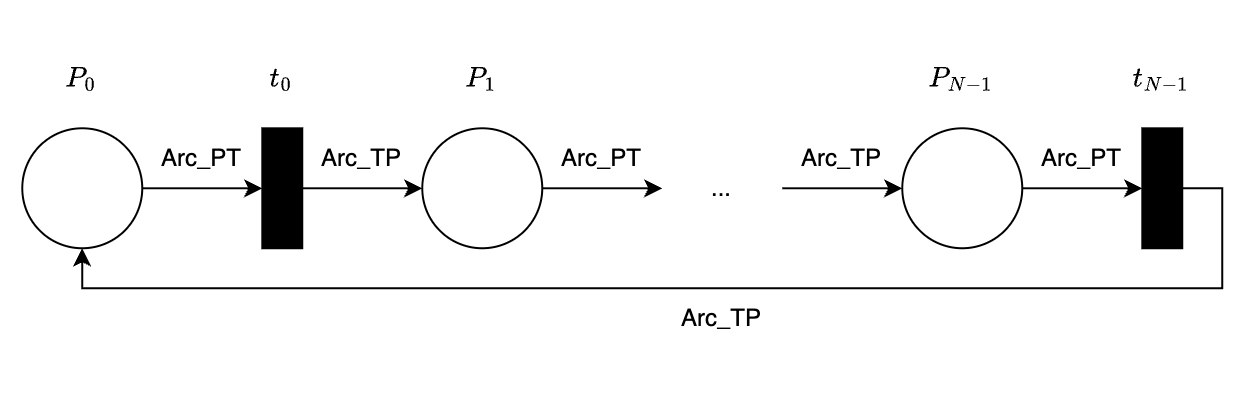
\includegraphics[width=0.6\textwidth]{img/scenario5/topo1.png}
\caption{Topologie 1 : chaîne cyclique}
\label{fig:sc5-topo1}
\end{figure}

Objets : $2N$. Arcs : $2N$ ($N$ \texttt{Arc\_PT} + $N$ \texttt{Arc\_TP}). Degré local de chaque n\oe{}ud : 1 entrant + 1 sortant — constant, indépendant de $N$.

\paragraph{Topologie 2 — Hub} ($N$ = 100, 500, 1\,000)

Une unique \texttt{Transition} centrale connectée à $N$ \texttt{Place}s distinctes (voir Figure~\ref{fig:sc5-topo2}).

\begin{figure}[h]
\centering
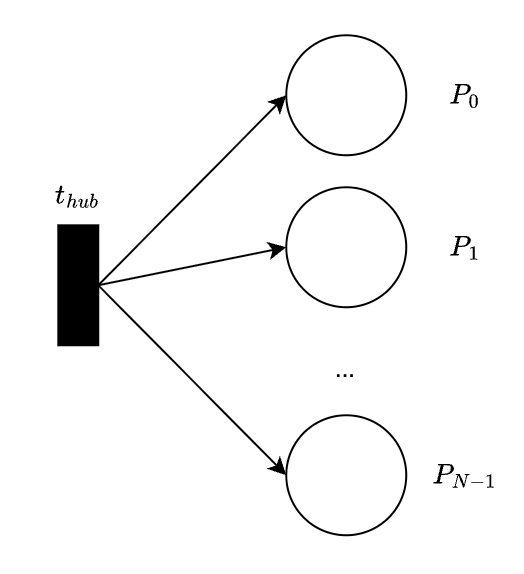
\includegraphics[width=0.25\textwidth]{img/scenario5/topo2.png}
\caption{Topologie 2 : hub central}
\label{fig:sc5-topo2}
\end{figure}

Objets : $N+1$. Arcs : $N$ \texttt{Arc\_TP}. Degré sortant du hub : $N$ — croissant linéairement.

% ----------------------------------------------------------------
\subsection{Résultats de référence (avant optimisation)}

\subsubsection{Création d'objets — chaîne cyclique (2N objets par modèle)}

Le tableau~\ref{tab:sc5-obj-cyclique} présente les médianes obtenues
pour la création de $2N$ objets en topologie cyclique.

\begin{table}[h]
\centering
\caption{Création d'objets --- chaîne cyclique. Médianes calculées sur
10 répétitions (mesures détaillées en annexe~\ref{ann:mesures-s5}).}
\label{tab:sc5-obj-cyclique}
\begin{tabular}{rrrr}
\hline
\textbf{N} & \textbf{Médiane (ms)} & \textbf{µs / objet} & \textbf{CV} \\
\hline
100    & 2,71   & 13,6 & 11,1\,\% \\
500    & 15,68  & 15,7 & 11,8\,\% \\
1\,000 & 26,14  & 13,1 & 16,3\,\% \\
5\,000 & 455,0\textsuperscript{$\dagger$} & 45,5 & 53\,\% \\
\hline
\end{tabular}
\end{table}

\textsuperscript{$\dagger$}\,À $N = 5\,000$, la distribution des dix
mesures est bimodale (5~runs $\approx$~200~ms, 5~runs $\approx$~700~ms),
reflétant l'\emph{entity manager bloat} d'OpenJPA discuté au
chapitre~\ref{chap:discussion}. Une mesure sur workspace fraîchement
initialisé donne $\approx 179$~ms (cohérent avec un coût intrinsèque de
$\sim$\,18~µs/objet).

Pour $N \leq 1\,000$, le coût par objet reste stable autour de
13--16~µs~: \texttt{\_createObject} est bien $O(N)$, conformément au
Scénario~2 (deux INSERTs JPA par objet, sans scan préalable).

\subsubsection{Création d'arcs — chaîne cyclique (2N arcs par modèle)}

Le tableau~\ref{tab:sc5-arc-cyclique} rapporte les temps de création
des arcs en topologie cyclique avant optimisation.

\begin{table}[h]
\centering
\caption{Création d'arcs --- chaîne cyclique, pré-Opt-5A. Médianes sur
10 répétitions (annexe~\ref{ann:mesures-s5}).}
\label{tab:sc5-arc-cyclique}
\begin{tabular}{rrrrc}
\hline
\textbf{N} & \textbf{Arcs} & \textbf{Médiane (ms)} & \textbf{µs / arc} & \textbf{T(N) / N²} \\
\hline
100   & 200     & 3,93       & 19,7  & $3{,}9 \times 10^{-4}$ \\
500   & 1\,000  & 41,57      & 41,6  & $1{,}7 \times 10^{-4}$ \\
1\,000 & 2\,000 & 154,71     & 77,4  & $1{,}5 \times 10^{-4}$ \\
5\,000 & 10\,000 & 4\,481,37 & 448,1 & $1{,}8 \times 10^{-4}$ \\
\hline
\end{tabular}
\end{table}

Le coût par arc double quand $N$ double, et $T(N)/N^2$ converge vers une constante pour $N \geq 500$ : signature d'un comportement $O(N^2)$.

\textit{Observation critique :} la chaîne cyclique, dont chaque n\oe{}ud a un degré local constant de 1, présente le même profil quadratique que le hub à fort degré. Ceci interdit une explication fondée sur la seule connectivité locale.

\subsubsection{Création d'arcs — hub (N arcs Arc\_TP, même n\oe{}ud)}

Le tableau~\ref{tab:sc5-arc-hub} présente les temps mesurés pour la
topologie hub avant optimisation.

\begin{table}[h]
\centering
\caption{Création d'arcs --- hub, pré-Opt-5A. Médianes sur 10
répétitions (annexe~\ref{ann:mesures-s5}).}
\label{tab:sc5-arc-hub}
\begin{tabular}{rrr}
\hline
\textbf{N} & \textbf{Médiane (ms)} & \textbf{µs / arc} \\
\hline
100   & 1,48  & 14,8 \\
500   & 15,72 & 31,4 \\
1\,000 & 63,82 & 63,8 \\
\hline
\end{tabular}
\end{table}

Même croissance $O(N^2)$. À $N = 1\,000$, hub et chaîne cyclique
affichent un coût par arc quasi-identique ($\sim$63--77~µs), révélant
un mécanisme interne commun dominant les deux topologies.

\subsubsection{Traversée — \texttt{getDefinition()} (chaîne cyclique)}

Les modèles cycliques contiennent $4N$ objets : $2N$ places et transitions auxquels s'ajoutent $2N$ \texttt{ConcreteRole}s, les rôles étant eux-mêmes des \texttt{ConcreteObject}s dans la définition du modèle. Le tableau~\ref{tab:sc5-traversal} rapporte les temps mesurés.

\begin{table}[h]
\centering
\caption{Traversée \texttt{getDefinition()} --- chaîne cyclique. Médianes
sur 10 répétitions (annexe~\ref{ann:mesures-s5}).}
\label{tab:sc5-traversal}
\begin{tabular}{rrrrr}
\hline
\textbf{N} & \textbf{Objets trouvés} & \textbf{Médiane (ms)} & \textbf{µs / objet} & \textbf{CV} \\
\hline
100    & 400     &  0,43 & 1,08 & 6,1\,\% \\
500    & 2\,000  &  1,96 & 0,98 & 4,1\,\% \\
1\,000 & 4\,000  &  4,21 & 1,05 & 5,2\,\% \\
5\,000 & 20\,000 & 20,42 & 1,02 & 5,7\,\% \\
\hline
\end{tabular}
\end{table}

La traversée est $O(N)$ à $\sim$1~µs/objet, avec un CV inférieur à 6\,\%
sur toutes les tailles --- parfaitement stable et insensible aux effets
de bloat observés sur la création.

% ----------------------------------------------------------------
\subsection{Analyse de la cause racine}

\subsubsection{Ce que la précondition fait réellement}

La précondition DbC pour \texttt{MANY\_TO\_MANY} dans
\texttt{ConcreteModel\_impl.precondition\_createRole} est la suivante
(Listing~\ref{ls-precond-m2m}).

\begin{lstlisting}[language=Java, firstnumber=386,
  caption={Précondition \texttt{MANY\_TO\_MANY} dans \texttt{precondition\_createRole}},
  label={ls-precond-m2m}]
case MANY_TO_MANY:
    final K_Object robject = range.getTarget();
    for (final K_Property p : domain.getTarget().getDomainOf(theMetaRole)) {
        if (p.getRange().equals(robject)) {
            throw new BadPreCondition(
                "The cardinality of the " + mr.getName()
                + " metarole is violated.");
        }
    }
    break;
\end{lstlisting}

\texttt{getDomainOf(theMetaRole)} itère \texttt{Object\_domainOf} — la liste des rôles \emph{locaux au n\oe{}ud domain} — filtrée par type de \texttt{MetaRole}. Pour la chaîne cyclique, chaque \texttt{Place} possède exactement une entrée \texttt{Arc\_PT} dans \texttt{Object\_domainOf} : le scan est $O(1)$ par appel, $O(N)$ au total. \textbf{La précondition n'est pas la source du $O(N^2)$} pour la topologie cyclique.

\subsubsection{La vraie cause : une asymétrie dans \texttt{\_createRole}}

La lecture en parallèle de \texttt{\_createObject} et \texttt{\_createRole} révèle une différence cruciale.

\texttt{\_createObject} (lignes 57--68 de \texttt{ConcreteModel\_impl}) effectue une \emph{insertion directe} (Listing~\ref{ls-createobject}).

\begin{lstlisting}[language=Java, firstnumber=57,
  caption={Insertion directe dans \texttt{\_createObject}},
  label={ls-createobject}]
private ConcreteObject_impl _createObject(MetaObject_impl metaobject) {
    try {
        final K_Object result = metaobject.getTarget().createObject();
        workspace.getDef_pt().createProperty(result, this.getTarget());
        return FactoryOfProxy.buildConcreteObject(result);
    } ...
}
\end{lstlisting}

\texttt{\_createRole} (lignes 331--345 et son overload ordonné lignes 419--436) passe quant à lui par \texttt{addInDefinition} (Listing~\ref{ls-createrole-avant}).

\begin{lstlisting}[language=Java, firstnumber=331,
  caption={Passage par \texttt{addInDefinition} dans \texttt{\_createRole} (avant optimisation)},
  label={ls-createrole-avant}]
private ConcreteRole_impl _createRole(MetaRole_impl mr,
        ConcreteObject_impl domain, ConcreteObject_impl range) {
    try {
        final K_PropertyType theMetaRole = mr.getMetaroleType();
        final K_Object result_o = mr.getTarget().createObject();
        theMetaRole.createProperty(result_o.getDataObject(),
                domain.getTarget(), range.getTarget());
        final ConcreteRole_impl result =
                FactoryOfProxy.buildConcreteRole(result_o);
        this.addInDefinition(result); // scan O(taille du modele)
        return result;
    } ...
}
\end{lstlisting}

\texttt{\_addInDefinition} appelle \texttt{\_isInDefinition} avant d'insérer (Listing~\ref{ls-addindef}).

\begin{lstlisting}[language=Java, firstnumber=80,
  caption={\texttt{\_addInDefinition} avec vérification préalable},
  label={ls-addindef}]
private ConcreteDef_impl _addInDefinition(ConcreteObject concreteobject) {
    final ConcreteObject_impl coi =
            concreteobject.narrow(ConcreteObject_impl.class);
    if (!_isInDefinition(coi)) {             // cache miss => scan O(N)
        getWorkspace().getDef_pt()
                .createProperty(coi.getTarget(), getTarget());
    }
    cache_isInDefinition.put(coi, true);
    return new ConcreteDef_impl(this, concreteobject);
}
\end{lstlisting}

\texttt{\_isInDefinition}, en cas de cache miss, itère toute la collection \texttt{Object\_rangeOf} du modèle pour vérifier si l'objet est déjà présent. Pour un \texttt{ConcreteRole} fraîchement créé, la réponse est toujours \texttt{false} — il vient d'être instancié et ne peut pas déjà figurer dans la définition. Le scan $O(\text{taille\_du\_modèle})$ est donc \textbf{systématiquement inutile} dans ce contexte.

Quand on crée le $j$-ième arc, le modèle contient déjà $2N + j$ membres ($2N$ objets + $j$ arcs déjà créés). Le scan coûte $O(2N+j)$. La somme sur les $2N$ arcs donne :

$$\sum_{j=0}^{2N-1}(2N+j) \approx 4N^2 + N^2 = 5N^2$$

Ce terme quadratique explique le comportement $O(N^2)$ observé pour les \emph{deux} topologies, indépendamment du degré local. L'asymétrie entre \texttt{\_createObject} (insertion directe) et \texttt{\_createRole} (passage par \texttt{\_addInDefinition}) est la cause racine.

% ----------------------------------------------------------------
\subsection{Optimisation Opt-5A : insertion directe dans \texttt{\_createRole}}

\subsubsection{Description}

Le correctif aligne \texttt{\_createRole} sur le pattern de \texttt{\_createObject} : pour un objet fraîchement créé, le scan \texttt{\_isInDefinition} est supprimé et remplacé par une insertion directe dans la définition du modèle, suivie d'une mise à jour du cache (Listing~\ref{ls-createrole-apres}).

\begin{lstlisting}[language=Java, firstnumber=331,
  caption={\texttt{\_createRole} après Opt-5A},
  label={ls-createrole-apres}]
private ConcreteRole_impl _createRole(MetaRole_impl mr,
        ConcreteObject_impl domain, ConcreteObject_impl range) {
    try {
        final K_PropertyType theMetaRole = mr.getMetaroleType();
        final K_Object result_o = mr.getTarget().createObject();
        theMetaRole.createProperty(result_o.getDataObject(),
                domain.getTarget(), range.getTarget());
        final ConcreteRole_impl result =
                FactoryOfProxy.buildConcreteRole(result_o);
        // result_o est neuf : _isInDefinition est toujours false
        workspace.getDef_pt().createProperty(result_o, this.getTarget());
        cache_isInDefinition.put(result, true);
        return result;
    } ...
}
\end{lstlisting}

Le même correctif est appliqué à l'overload ordonné de \texttt{\_createRole} (ligne 419).

\subsubsection{Propriétés}

\begin{itemize}
  \item \textbf{Correction :} \texttt{result\_o} est créé par \texttt{mr.getTarget().createObject()} — il ne peut pas déjà figurer dans la définition. La suppression du scan est sémantiquement équivalente.
  \item \textbf{DbC :} la précondition \texttt{precondition\_createRole} n'est pas modifiée. Les garanties d'unicité des paires (domaine, cible) restent intégralement assurées.
  \item \textbf{Cache :} la cohérence du \texttt{WeakHashMap} est maintenue via \texttt{cache\_isInDefinition.put(result, true)}, comme dans \texttt{\_addInDefinition}.
  \item \textbf{Portée :} les deux overloads de \texttt{\_createRole} sont corrigés (arcs non ordonnés et ordonnés), soit 4 lignes modifiées au total.
\end{itemize}

% ----------------------------------------------------------------
\subsection{Résultats après optimisation}

\subsubsection{Chaîne cyclique — création d'arcs}

Le tableau~\ref{tab:sc5-arc-cyclique-apres} compare les médianes
avant et après Opt-5A pour la topologie cyclique.

\begin{table}[h]
\centering
\caption{Création d'arcs --- chaîne cyclique, avant et après Opt-5A.
Médianes calculées sur 10 répétitions par campagne
(annexe~\ref{ann:mesures-s5}).}
\label{tab:sc5-arc-cyclique-apres}
\begin{tabular}{rrrrrr}
\hline
\textbf{N} & \textbf{Avant (ms)} & \textbf{Après (ms)} & \textbf{Gain}
           & \textbf{µs/arc avant} & \textbf{µs/arc après} \\
\hline
100    & 3,93       & 3,89      & $\approx 1\times$ & 19,7  & 19,4 \\
500    & 41,57      & 22,02     & $1{,}89\times$    & 41,6  & 22,0 \\
1\,000 & 154,71     & 70,58     & $2{,}19\times$    & 77,4  & 35,3 \\
5\,000 & 4\,481,37  & 1\,021,23 & $4{,}39\times$    & 448,1 & 102,1 \\
\hline
\end{tabular}
\end{table}

Le gain s'accentue avec $N$ --- comportement attendu d'une correction
$O(N^2) \rightarrow O(f(N))$ avec $f(N)$ sous-quadratique.

\textit{Note sur la variabilité à grand $N$ :} la base de données de test
est partagée entre exécutions (singleton \texttt{TestWorkspace}). Au fil
des répétitions, la session OpenJPA accumule des entités persistées par
les exécutions antérieures, ce qui se traduit par un CV plus élevé sur
les phases de création post-Opt-5A ($\sim$\,14\,\% à $N=5\,000$). La
campagne pré-Opt-5A, réalisée immédiatement après revert d'Opt-5A,
montre une stabilité remarquable (CV de 2,8\,\% à $N=5\,000$).

\subsubsection{Complexité résiduelle --- chaîne cyclique}

En comparant les médianes post-Opt-5A à $N = 500$ et $N = 1\,000$~:

$$\frac{T_{\text{arc}}(1\,000)}{T_{\text{arc}}(500)} = \frac{70{,}58}{22{,}02} \approx 3{,}20$$

Pour $O(N)$ pur, on attendrait $2{,}0\times$~; pour $O(N \log N)$,
$\sim 2{,}2\times$~; pour $O(N^2)$, $4{,}0\times$. Le ratio observé
$3{,}20$ se situe entre $O(N \log N)$ et $O(N^2)$~: l'optimisation a
éliminé le coût algorithmique principal mais le plancher mesuré reste
supérieur à $O(N \log N)$ théorique. Cet écart s'explique par la
contribution résiduelle des INSERTs JPA sur l'index B-tree de H2
(chaque insertion dans un index de taille $k$ coûte $O(\log k)$) cumulée
au bruit lié à l'\emph{entity manager bloat} (chapitre~\ref{chap:discussion})~:
le plancher empirique est donc proche de $O(N \log N)$ asymptotique, sans
l'atteindre exactement dans l'environnement de mesure utilisé.

\subsubsection{Hub — création d'arcs}

Le tableau~\ref{tab:sc5-arc-hub-apres} présente le même comparatif
pour la topologie hub.

\begin{table}[h]
\centering
\caption{Création d'arcs --- hub, avant et après Opt-5A. Médianes
calculées sur 10 répétitions par campagne (annexe~\ref{ann:mesures-s5}).}
\label{tab:sc5-arc-hub-apres}
\begin{tabular}{rrrr}
\hline
\textbf{N} & \textbf{Avant (ms)} & \textbf{Après (ms)} & \textbf{Gain} \\
\hline
100    &  1,48 &  1,55 & $\approx 1\times$ \\
500    & 15,72 & 10,99\textsuperscript{$\dagger$} & $1{,}43\times$ \\
1\,000 & 63,82 & 36,16 & $1{,}77\times$    \\
\hline
\end{tabular}
\end{table}

\textsuperscript{$\dagger$}\,À $N=500$, la distribution est bimodale
(six runs $\sim$\,10~ms, quatre runs $\sim$\,34~ms)~; la médiane reflète
la moitié inférieure du cluster.

Le hub bénéficie également du correctif ($\sim$\,1,5--1,7$\times$), mais
reste $O(N^2)$~: la précondition \texttt{MANY\_TO\_MANY} itère désormais
seule \texttt{hub.getDomainOf(Arc\_TP)}, dont la taille croît linéairement
avec le degré. Au $i$-ième arc, le scan coûte $O(i)$~; la somme donne
$O(N^2)$. La mesure confirme cette prédiction~:

$$\frac{N(N-1)}{2}\bigg|_{N=1000} \approx 500\,000 \text{ opérations} \times 72\text{ ns/op} \approx 36{,}0\text{ ms} \quad \text{(mesuré : 36,2~ms)}$$

% ----------------------------------------------------------------
\subsection{Synthèse}

Le tableau~\ref{tab:sc5-synthese} récapitule l'impact d'Opt-5A sur les
deux topologies, les complexités résiduelles et les invariants préservés.

\begin{table}[h]
\centering
\caption{Synthèse Opt-5A. Médianes calculées sur 10 répétitions.}
\label{tab:sc5-synthese}
\begin{tabular}{lll}
\hline
\textbf{Métrique} & \textbf{Avant Opt-5A} & \textbf{Après Opt-5A} \\
\hline
Cyclique --- complexité arcs & $O(N^2)$ & $\sim O(N \log N)$ --- plancher JPA \\
Hub --- complexité arcs      & $O(N^2)$ & $O(N^2)$ --- précondition MANY\_TO\_MANY \\
Cyclique, $N=1\,000$ arcs    & 155 ms     & \textbf{71 ms} ($2{,}19\times$) \\
Cyclique, $N=5\,000$ arcs    & 4\,481 ms  & \textbf{1\,021 ms} ($4{,}39\times$) \\
Traversée                    & $O(N)$, $\sim$1~µs/objet & inchangée \\
DbC                          & intact     & intact \\
Lignes modifiées             & ---        & 4 lignes, 2 méthodes \\
\hline
\end{tabular}
\end{table}

% ----------------------------------------------------------------
\subsection{Bottleneck résiduel — hub (non implémenté)}

Pour ramener la topologie hub à $O(N \log N)$, il faudrait un second correctif dans \texttt{pre\-con\-di\-tion\_crea\-te\-Role} : remplacer l'itération de \texttt{getDomainOf(theMetaRole)} par un lookup $O(1)$ dans un index maintenu dans \texttt{ConcreteModel\_impl} (Listing~\ref{ls-roleindex}).

\begin{lstlisting}[language=Java,
  caption={Index proposé pour \texttt{precondition\_createRole} MANY\_TO\_MANY},
  label={ls-roleindex}]
// Dans ConcreteModel_impl
private final Map<K_PropertyType,
                  Map<K_Object, Set<K_Object>>> roleIndex = new HashMap<>();

// Dans precondition_createRole, cas MANY_TO_MANY :
Set<K_Object> ranges = roleIndex
    .getOrDefault(theMetaRole, Collections.emptyMap())
    .getOrDefault(domain.getTarget(), Collections.emptySet());
if (ranges.contains(range.getTarget())) {
    throw new BadPreCondition("...");
}

// Dans _createRole, apres l'insertion :
roleIndex.computeIfAbsent(theMetaRole, k -> new HashMap<>())
         .computeIfAbsent(domain.getTarget(), k -> new HashSet<>())
         .add(range.getTarget());
\end{lstlisting}

Cette approche nécessite une initialisation \emph{lazy} de l'index lors de la première vérification pour les modèles chargés depuis la base, ainsi qu'une invalidation à la suppression de rôles. L'implémentation est plus invasive et sort du périmètre du présent scénario.

% ----------------------------------------------------------------
\subsection{Conclusion}

Le Scénario~5 révèle et corrige une inefficacité cachée dans la création de rôles de MetaDONE. La cause racine est une asymétrie de conception entre \texttt{\_createObject} (insertion directe en $O(1)$) et \texttt{\_createRole} (passage par \texttt{\_addInDefinition} $\rightarrow$ scan $O(\text{taille\_du\_modèle})$), rendant toute création de rôle $O(N^2)$ quelle que soit la topologie du modèle.

L'optimisation Opt-5A, réalisée dans deux méthodes de \texttt{ConcreteModel\_impl}, aligne \texttt{\_createRole} sur \texttt{\_createObject} en supprimant un scan systématiquement inutile pour des objets fraîchement créés. Elle réduit la complexité de la création d'arcs de $O(N^2)$ à un plancher proche de $O(N \log N)$ pour les topologies à degré borné, avec un gain empirique médian de $2{,}19\times$ à $N = 1\,000$ et $4{,}39\times$ à $N = 5\,000$ (mesuré sur 10 répétitions par campagne). La sémantique DbC est intégralement préservée.

Pour les tailles de modèles typiques de MetaDONE ($N < 200$), les performances étaient déjà acceptables. Le bénéfice est significatif dès $N \geq 500$ et devient critique à $N = 5\,000$, où la création de $10\,000$ arcs en chaîne cyclique passe de $4\,481$~ms à $1\,021$~ms (cf.~tableau~\ref{tab:sc5-arc-cyclique-apres}), rendant la construction de grands modèles de vérification formelle praticable dans un contexte interactif.



\chapter{Discussion}
\label{chap:discussion}

% ----------------------------------------------------------------
\section{Synthèse des résultats}

Les scénarios réalisés couvrent quatre axes du comportement de MetaDONE~: la construction de métamodèles (S1), le chargement de scripts GraSyLa (S2), la boucle de dispatch de visualisation (S4) et la scalabilité de la création de modèles concrets (S5). Deux optimisations ont été implémentées et validées~; deux candidates ont été écartées pour des raisons distinctes. Le Tableau~\ref{tab:disc-bilan} synthétise l'ensemble des décisions.

\begin{table}[h]
\centering
\small
\caption{Bilan des optimisations étudiées}
\label{tab:disc-bilan}
\begin{tabular}{p{2.5cm}p{4.8cm}p{2.4cm}p{3cm}}
\hline
\textbf{Scénario} & \textbf{Problème identifié} & \textbf{Décision} & \textbf{Résultat} \\
\hline
S1 & \texttt{\_isInDefinition} $O(N^2)$ dans \texttt{getMOByName} &
   Implémenté (\texttt{WeakHashMap}) & $O(N^2) \rightarrow O(N)$ \\[4pt]
S2 --- candidate batch-JPA & Batch JPA (\texttt{batchLimit}) &
   Écartée & Aucun effet sur H2 local \\[4pt]
S2 --- candidate bypass-précondition & Bypass de \texttt{precondition\_createRole} &
   Écartée & Violation DbC \\[4pt]
S4 & Dispatch $O(N \times M \times K)$ &
   Non implémenté & Déjà efficace à l'échelle réelle \\[4pt]
S5 --- Opt-5A & \texttt{\_createRole} $O(N^2)$ via \texttt{\_addInDefinition} &
   Implémenté & $O(N^2) \rightarrow$ plancher $\sim O(N \log N)$ \\
\hline
\end{tabular}
\end{table}

Les deux optimisations retenues partagent un même schéma : elles éliminent un scan systématiquement redondant par analyse statique des invariants du programme. Dans les deux cas, la correction est locale (quelques lignes), non invasive pour le reste de l'API, et préserve intégralement les garanties Design by Contract. Ce pattern — identifier un scan $O(N)$ appelé $O(N)$ fois par invariant toujours vrai — constitue la contribution technique principale de ce travail.

% ----------------------------------------------------------------
\section{Deux patterns d'optimisation distincts}

L'analyse des scénarios fait émerger deux familles de problèmes de performance dans MetaDONE.

\paragraph{Structures de données inadaptées à leur usage.}
La première famille correspond à l'utilisation d'une collection linéaire là où un dictionnaire serait approprié. C'est le cas du Scénario~1, où \texttt{\_isInDefinition} itérait la liste de définition du modèle à chaque appel alors qu'un \texttt{WeakHashMap} fournit la même information en $O(1)$. Cette famille de problèmes est classique en ingénierie logicielle et sa correction est généralement peu risquée.

\paragraph{Asymétries de conception non documentées.}
La seconde famille est plus subtile : deux méthodes apparentées adoptent des stratégies d'insertion divergentes sans justification fonctionnelle visible. En Scénario~5, \texttt{\_createObject} contournait \texttt{\_addInDefinition} par une insertion directe ($O(1)$), tandis que \texttt{\_createRole} passait par la vérification complète ($O(N)$). Ce type de divergence silencieuse est difficile à détecter par revue de code seule. Il a fallu un benchmark avec deux topologies — dont l'une invalide l'hypothèse initiale (la chaîne cyclique, supposée $O(N)$, présentant le même $O(N^2)$ que le hub) — pour localiser la cause racine. Ce résultat illustre la valeur des benchmarks paramétriques comme outil de diagnostic, au-delà du simple profilage.

% ----------------------------------------------------------------
\section{Le Design by Contract comme contrainte architecturale}

Le rejet de la \textbf{candidate bypass-précondition} (section~\ref{sec:scenario2-precondition-rejet}) mérite une discussion particulière. La proposition consistait à introduire une méthode \texttt{createRoleTrusted} court-circuitant \texttt{precondition\_createRole} pour les appelants ayant préalablement vérifié les contraintes de cardinalité. Bien que le gain de performance fût plausible --- la précondition représentait une fraction non négligeable du temps de chargement d'un script BPMN --- cette option a été écartée pour violation du principe Design by Contract (DbC) sur lequel repose l'architecture de MetaDONE.

Ce choix révèle une tension structurelle entre performance et correction par construction. Dans MetaDONE, les préconditions ne sont pas de simples validations défensives optionnelles : elles constituent la formalisation des invariants du métamodèle (cardinalités, unicité des rôles, appartenance au modèle). Les lever sélectivement, même dans un contexte maîtrisé, fragilise le modèle de confiance que le DbC instaure entre les couches de l'architecture.

L'optimisation correcte — comme le montre Opt-5A — consiste à démontrer qu'un invariant \emph{plus fort} que la précondition est déjà garanti par le contexte d'appel (un objet fraîchement créé ne peut pas être dans la définition), et à exploiter cet invariant plutôt qu'à supprimer la vérification. Cette leçon est généralisable : dans un système à fortes garanties formelles, les optimisations les plus sûres sont celles qui raisonnent \emph{sur} les invariants plutôt que celles qui les contournent.

% ----------------------------------------------------------------
\section{Hypothèse simplificatrice : la persistance JPA/H2}
\label{sec:disc-jpa}

Ce travail exclut explicitement l'optimisation de la couche de persistance — schéma JPA, configuration H2, indexation des tables. Cette exclusion constitue une hypothèse simplificatrice dont les implications doivent être discutées.

\subsection*{Ce que cette hypothèse implique pour les mesures}

Toutes les durées mesurées incluent le coût des opérations JPA dans leur configuration actuelle. En particulier, les collections \texttt{Object\_domainOf} et \texttt{Object\_rangeOf} sont des \texttt{LinkedList<K\_Property>} chargées en mémoire par OpenJPA et parcourues séquentiellement. Si ces parcours passaient par des requêtes JPQL exploitant des index composites \texttt{(Property\_domain, Property\_type)} et \texttt{(Property\_range, Property\_type)}, le coût de chaque accès filtré serait $O(\log N)$ au lieu de $O(\text{degré\_total})$.

Le plancher résiduel observé après Opt-5A pour la chaîne cyclique (entre $O(N \log N)$ et $O(N^2)$ selon les mesures) est, lui, inhérent à tout système de stockage persistant indexé~: chaque INSERT met à jour un B-tree dont la hauteur croît comme $\log N$. La contribution mesurable au-delà de $O(N \log N)$ est imputable à l'\emph{entity manager bloat} d'OpenJPA (discuté à la section~\ref{sec:validite-mesures}) et n'est pas une limitation propre à l'algorithmique de MetaDONE.

\subsection*{Justification du choix}

Trois raisons motivent cette exclusion. Premièrement, le schéma JPA de MetaDONE — modèle universel à deux tables (\texttt{K\_Object} et \texttt{K\_Property}) — est une décision architecturale fondamentale qui conditionne l'extensibilité du système ; toute modification du schéma interagirait avec l'ensemble des backends supportés (JPA2, ObjectDB). Deuxièmement, les gains réalisables par optimisation de l'algorithmique Java — $O(N^2) \rightarrow O(N \log N)$ en S5, $O(N^2) \rightarrow O(N)$ en S1 — sont d'un ordre de grandeur supérieur à ce qu'une indexation SQL pourrait apporter à elle seule. Troisièmement, les optimisations implémentées opèrent en mémoire et restent valides quelle que soit la configuration du backend de persistance.

\subsection*{Pistes d'optimisation base de données}

À titre de perspective, une ligne de travail naturelle consisterait à remplacer les parcours de \texttt{getDomainOf(theMetaRole)} filtrés par type — utilisés notamment dans \texttt{precondition\_createRole} \texttt{MANY\_TO\_MANY} — par des requêtes JPQL paramétrées avec index. Cela convertirait le bottleneck résiduel du hub ($O(N^2)$) en $O(N \log N)$, au prix de modifications dans la couche repository. Ce travail sort du périmètre du présent mémoire mais représente la suite logique des optimisations ici entreprises.

% ----------------------------------------------------------------
\section{Validité des mesures et contexte d'exécution}
\label{sec:validite-mesures}

Les benchmarks ont été réalisés en mode standalone JUnit, en dehors du contexte Eclipse RCP et de son thread UI. Ce choix présente un compromis entre contrôlabilité et représentativité.

\subsection*{Avantages}

L'environnement standalone est reproductible, isolé des artefacts de rendu Eclipse, et permet de mesurer précisément les couches métier (\texttt{metabusiness}, repository JPA) sans bruit d'interface graphique. Il est particulièrement adapté aux scénarios S1, S2 et S5, qui portent sur des opérations de modélisation (création d'objets, de rôles, chargement de scripts).

\subsection*{Limites}

Le benchmark standalone du Scénario~4 ne couvre que les étapes 1 et 2 du pipeline de rendu GraSyLa (récupération des équations, évaluation de \texttt{hasType()}). L'étape~3 --- évaluation de l'arbre d'expression (appels JavaScript via Rhino, accès aux propriétés du modèle pour calculer couleurs, positions, étiquettes) --- requiert la couche Eclipse UI et n'est pas isolable dans un test JUnit. Pour combler ce manque, une session de profilage live de l'application Eclipse complète a été réalisée et présentée à la section~\ref{sec:sc4-live}~: elle quantifie le poids effectif des trois étapes en contexte interactif réel. Les deux types de mesures (standalone et live) reposent toutefois sur des protocoles distincts et ne sont pas strictement comparables~; la quantification de l'étape~3 reste donc indirecte et doit être lue comme un ordre de grandeur.

Par ailleurs, les benchmarks utilisent un projet de test partagé par l'ensemble des scénarios (\texttt{TestWorkspace} singleton, base H2 persistante). La croissance de la session JPA entre les exécutions introduit un biais sur les mesures à grand $N$, comme l'illustre la dégradation de la création d'objets à $N = 5\,000$ entre la mesure avant et après Opt-5A. Ce phénomène, connu sous le terme d'\emph{entity manager bloat}, est une limite documentée des benchmarks intégrés sur longue durée. Pour des mesures absolues plus fiables, chaque scénario devrait être exécuté sur une base fraîche.

Enfin, aucune phase de \textit{warmup} de la JVM n'a été instaurée avant les mesures. La compilation JIT du HotSpot peut rendre les premières exécutions d'une méthode chaude significativement plus lentes que son régime stabilisé. Trois éléments permettent toutefois de conclure que cette limite n'invalide pas les ordres de grandeur des gains observés. \emph{Premièrement}, la médiane sur 10 répétitions absorbe naturellement les valeurs aberrantes des premières exécutions liées à la compilation initiale~: avec 10 mesures, jusqu'à 4 valeurs hautes peuvent être ignorées sans biais. \emph{Deuxièmement}, les coefficients de variation rapportés sont faibles sur la majorité des scénarios (typiquement $< 6\,\%$ pour les phases de traversée et les mesures à $N \leq 1\,000$), ce qui constitue une preuve empirique de la stabilisation du régime d'exécution. \emph{Troisièmement}, les gains des deux optimisations retenues (Opt-1 et Opt-5A) sont d'ampleur suffisante --- respectivement passage de $O(N^2)$ à $O(N)$, et facteur $\times 4{,}39$ à $N = 5\,000$ --- pour qu'un éventuel biais de JIT (de l'ordre de quelques pourcents sur les premières mesures) ne puisse inverser ni masquer la tendance. En revanche, pour des comparaisons fines entre micro-optimisations dont l'amplitude attendue serait inférieure à $20\,\%$, une procédure formelle de warmup --- par exemple via JMH ou en suivant les recommandations méthodologiques de \cite{georges2007statistically} --- deviendrait indispensable.

% ----------------------------------------------------------------
\section{Perspectives}

\paragraph{À court terme — mise en cache de \texttt{getEquations()}.}
La méthode \texttt{GrasylaScript.getEquations()} reconstruit l'intégralité des wrappers \texttt{GrasylaEquation} depuis JPA à chaque appel (coût médian mesuré en S4 : 3,70~ms pour 106 équations sur 10 répétitions). Dans une boucle de rendu à 30 images par seconde, ce surcoût fixe représente $\sim$\,111~ms/s, indépendamment de la taille du modèle. Un mécanisme d'invalidation existe déjà via \texttt{notifyScriptChanged()} ; l'ajout d'un champ \texttt{volatile} mis à \texttt{null} lors de chaque notification suffirait à éliminer ce coût. Il s'agit de l'optimisation à plus fort rapport gain/effort parmi celles identifiées mais non implémentées dans ce travail.

\paragraph{À moyen terme — index de précondition pour les n\oe{}uds à fort degré.}
Le bottleneck résiduel identifié en S5 pour la topologie hub ($O(N^2)$, dû à la précondition \texttt{MANY\_TO\_MANY}) pourrait être corrigé par un index \texttt{Map<MetaRole, Map<K\_Object, Set<K\_Object>>>} maintenu dans \texttt{ConcreteModel\_impl}, ramenant la vérification de $O(\text{degré})$ à $O(1)$. L'implémentation requiert une gestion de cohérence à la suppression de rôles et une initialisation \emph{lazy} pour les modèles chargés depuis la base. Ce travail s'appuie directement sur l'analyse menée en S5 et constitue un prolongement naturel d'Opt-5A.

\paragraph{À plus long terme — profilage du pipeline de rendu complet.}
La question du coût de rendu complet (évaluation des expressions GraSyLa, pipeline graphique Eclipse) reste ouverte. Un profilage \emph{async-profiler} attaché à une instance Eclipse en cours d'exécution, sur un modèle BPMN de taille réaliste, permettrait de situer le dispatch et l'évaluation d'expressions dans le budget-temps total d'une frame de rendu, et d'identifier si des optimisations algorithmiques au niveau de l'interpréteur GraSyLa sont justifiées.

Enfin, l'abandon de l'option sérialisation — remplacement de JPA par un format binaire personnalisé — mérite d'être mentionné comme alternative architecturale à long terme. Si MetaDONE devait évoluer vers des modèles de taille significativement plus grande, un mécanisme de persistance non relationnel pourrait lever le plancher $O(\log N)$ inhérent aux index B-tree. Ce choix impliquerait cependant une rupture partielle avec la portabilité multi-backend que le modèle JPA actuel assure.

\chapter{Conclusion}
\label{chap:conclusion}

% ----------------------------------------------------------------
\section{Bilan de la recherche}

Ce mémoire s'est donné pour objectif d'identifier, de mesurer et de réduire les
goulots de performance de MetaDONE, un outil MetaCASE bâti sur l'architecture
MetaL$_2$ et reposant sur une couche de persistance JPA. La démarche adoptée a
suivi un cycle empirique complet pour chacun des quatre scénarios étudiés~:
conception d'un benchmark instrumenté, mesure de référence, identification de
la cause racine dans le code source, conception et implémentation d'une
optimisation, vérification expérimentale du gain.

Cette méthodologie a guidé toutes les décisions techniques, y compris les
décisions négatives. Sur les quatre optimisations candidates initialement
identifiées, deux ont été \emph{rejetées} sur la base des mesures~:
la candidate \og batch-JPA \fg{} (activation du paramètre \texttt{batchLimit}),
sans effet sur une base H2 embarquée, et la candidate \og bypass-précondition \fg{}
(introduction d'une méthode \texttt{createRoleTrusted} contournant
\texttt{precondition\_createRole}), incompatible avec le principe Design by
Contract structurant l'architecture de MetaDONE. %Ces refus documentés délimitent l'espace des solutions acceptables et constituent à part entière un résultat de la recherche.

% ----------------------------------------------------------------
\section{Contribution}

La contribution technique principale de ce travail se résume en deux
optimisations algorithmiques implémentées et validées.

L'optimisation du Scénario~1 introduit un cache \texttt{WeakHashMap} dans
\texttt{ConcreteModel\_impl.\_isInDefinition}, éliminant un scan linéaire
répété de la liste de définition. La complexité de \texttt{getMOByName} passe
de $O(N^2)$ à $O(N)$.

L'optimisation Opt-5A du Scénario~5 corrige une asymétrie non documentée entre
\texttt{\_createObject} (insertion directe en $O(1)$) et \texttt{\_createRole}
(passage par un scan en $O(\text{taille\_du\_modèle})$). En quatre lignes
modifiées, la création d'arcs passe de $O(N^2)$ à un plancher proche de
$O(N \log N)$ pour les topologies à degré borné, avec un gain médian de
$2{,}19\times$ à $N = 1\,000$ et $4{,}39\times$ à $N = 5\,000$ (mesuré sur
10 répétitions par campagne). La borne résiduelle correspond au plancher inhérent à tout
backend de persistance indexé.

Au-delà des chiffres, ce travail dégage trois enseignements généralisables.
Premièrement, les bottlenecks les plus impactants ne se trouvent pas
toujours là où l'intuition les place : la mise en évidence de la complexité
$O(N^2)$ de \texttt{\_createRole} n'a été possible qu'en comparant deux
topologies dont l'une infirmait l'hypothèse initiale. Deuxièmement, dans
un système à garanties formelles, les optimisations les plus sûres sont celles
qui \emph{exploitent} les invariants plutôt que celles qui les contournent~:
l'opposition entre la candidate \og bypass-précondition \fg{} (rejetée) et
Opt-5A (retenue) en est l'illustration.
Troisièmement, l'explicitation des hypothèses simplificatrices — ici,
l'exclusion délibérée de l'optimisation du schéma JPA — est essentielle à
l'interprétation correcte des résultats.

% ----------------------------------------------------------------
\section{Limites du travail et points de vigilance}

Plusieurs limites doivent être signalées pour délimiter la portée des résultats présentés.

\paragraph{Périmètre instrumenté.}
Les benchmarks ont été réalisés en mode standalone JUnit, hors du contexte
Eclipse RCP. Si ce choix offre une excellente contrôlabilité pour les couches
métier et repository (Scénarios 1, 2 et 5), il a empêché de mesurer
directement l'étape~3 du pipeline de visualisation (évaluation des expressions
GraSyLa). Cette limite a été compensée a posteriori par un profilage live de
l'application Eclipse via async-profiler (Section~\ref{sec:sc4-live}), mais
les deux types de mesures ne sont pas strictement comparables et la
quantification reste indirecte.

\paragraph{Biais d'accumulation JPA.}
La base de test étant partagée entre exécutions, la session OpenJPA accumule
des entités au fil des scénarios. Ce phénomène (\emph{entity manager bloat}) a
été observé à $N = 5\,000$ en S5 et a légèrement biaisé les valeurs absolues
mesurées. Les comparaisons relatives avant/après optimisation restent valides,
mais les valeurs absolues à grand $N$ doivent être interprétées avec
prudence. Une réexécution sur base fraîche pour chaque scénario améliorerait
la fiabilité des chiffres absolus.

\paragraph{Hypothèse simplificatrice sur la persistance.}
L'optimisation du schéma JPA et des index SQL a été explicitement exclue du
périmètre. Cette exclusion, motivée par la portée architecturale d'une telle
modification, signifie que le plancher proche de $O(N \log N)$ observé en S5
après Opt-5A reflète une contrainte du backend (mise à jour d'index B-tree à
chaque INSERT) non remise en cause dans ce travail.

\paragraph{Si c'était à refaire.}
Avec le recul, deux choix méthodologiques mériteraient d'être révisés. D'une
part, le profilage live aurait dû être réalisé plus tôt dans le processus :
les 11~\% de coût attribués à \texttt{getEquations}/\texttt{hasType} en
contexte interactif (contre $\sim 0\,\%$ en standalone) n'ont été révélés
qu'en fin de travail et auraient pu orienter différemment les priorités.
D'autre part, l'effort consacré à l'évaluation des candidates batch-JPA et
bypass-précondition (finalement rejetées) aurait pu être mieux dimensionné
avec une lecture préalable plus attentive de la configuration H2 et du
contrat DbC.
Ces deux constats relèvent toutefois davantage d'un apprentissage que d'une
remise en cause de la démarche d'ensemble.

% ----------------------------------------------------------------
\section{Pistes non explorées et perspectives}

Plusieurs pistes de réflexion identifiées au cours du travail n'ont pu être
développées, soit par manque de temps, soit par dépassement du périmètre
défini. Elles méritent toutefois d'être signalées pour orienter des travaux
ultérieurs.

\paragraph{Mise en cache de \texttt{getEquations()} — court terme.}
Le profilage live a mesuré que cette méthode représente 11,16~\% du temps CPU
en contexte interactif, car elle reconstruit l'intégralité des 106 wrappers
\texttt{GrasylaEquation} à chaque cycle de rendu. Un mécanisme de cache
volatile invalidé par \texttt{notifyScriptChanged()} suffirait à éliminer ce
surcoût en quelques lignes de code. C'est la piste au rapport gain/effort le
plus favorable parmi celles identifiées.

\paragraph{Index de précondition pour \texttt{MANY\_TO\_MANY} — moyen terme.}
Le bottleneck résiduel identifié en S5 pour les topologies à fort degré
(complexité $O(N^2)$ due à la vérification de l'unicité des paires) pourrait
être corrigé par un index $\texttt{Map<MetaRole, Map<K\_Object,
Set<K\_Object>>>}$ maintenu dans \texttt{ConcreteModel\_impl}. L'implémentation
requiert une gestion de cohérence à la suppression et une initialisation
\emph{lazy} pour les modèles chargés.

\paragraph{Optimisation de la couche de persistance — long terme.}
L'introduction d'index composites SQL sur \texttt{(Property\_domain,
Property\_type)} convertirait certains scans $O(\text{degré})$ en $O(\log N)$.
Cette piste relève cependant d'un projet à part entière, interagissant avec
l'ensemble des backends supportés. Le promoteur a souligné que, dans le scope
de ce mémoire, l'option ORM/SQL restant la voie de persistance par défaut,
l'optimisation de la base de données constituera \emph{une étape inévitable}
pour tout travail ultérieur visant un passage à l'échelle significatif.

\paragraph{Reconstruction incrémentale de la scène GraSyLa.}
Le profilage live a révélé que les $\approx 53\,\%$ de temps CPU passés dans la
boucle \texttt{trigger}~$\rightarrow$~\texttt{buildComponent}~$\rightarrow$~%
\texttt{evaluateComponent} proviennent d'une reconstruction \emph{globale} de
la scène à chaque modification du modèle. Une stratégie de reconstruction
incrémentale, ciblée sur les seuls composants affectés, semble la piste à plus
fort potentiel pour les améliorations futures de l'interface graphique.

% ----------------------------------------------------------------
\section*{}

MetaDONE est un outil dont l'architecture privilégie l'extensibilité, la
généricité et la correction formelle ; cette généricité a un coût, qu'aucune
optimisation locale ne peut entièrement effacer. Le travail présenté ici ne
prétend pas refonder cette architecture, mais en améliorer le comportement
empirique aux points où une analyse rigoureuse révèle une marge d'amélioration
réelle. Les deux optimisations retenues — toutes deux locales, peu invasives,
et préservant intégralement les garanties du Design by Contract — démontrent
qu'un gain substantiel de performance est compatible avec le respect des
principes architecturaux fondateurs de l'outil.



%\chapter{ Bibliographie ou Références}
\bibliographystyle{ACM-Reference-Format}
\bibliography{biblio}


\part*{Annexes}
%\addcontentsline{toc}{part}{Annexes}
 
\appendix
\chapter{Mesures brutes}
\label{ann:mesures}

\section{Scénario 1 — Construction du métamodèle BPMN}
\label{ann:mesures-s1-a}

Toutes les mesures du Scénario~1 portent sur le temps total de construction
du métamodèle BPMN au démarrage de l'application. Les optimisations Opt-1
à Opt-4 sont introduites cumulativement (chapitre~\ref{chap:developpement},
sections~\ref{sec:opti-metamodel} et~\ref{sec:scenario1-opti2}). Opt-1
n'étant pas mesurable indépendamment (il s'agit de la simple activation
du cache, dont l'effet n'apparaît qu'à partir d'Opt-2), seules les
quatre configurations \emph{baseline}, après Opt-2, après Opt-3 et après
Opt-4 sont reportées ci-dessous.

\subsection*{Baseline (avant toute optimisation)}

\begin{table}[h]
\centering
\caption{Scénario 1 --- Baseline. 10 répétitions, temps total en secondes.}
\begin{tabular}{rr}
\hline
\textbf{Run} & \textbf{Temps (s)} \\
\hline
1  & 18,570 \\
2  & 18,150 \\
3  & 17,968 \\
4  & 17,693 \\
5  & 18,114 \\
6  & 18,650 \\
7  & 17,673 \\
8  & 18,434 \\
9  & 18,246 \\
10 & 18,309 \\
\hline
\textbf{Médiane} & \textbf{18,198} \\
Moyenne          & 18,181 \\
Min              & 17,673 \\
Max              & 18,650 \\
CV               & 1,8\,\% \\
\hline
\end{tabular}
\end{table}

\subsection*{Après application cumulative des optimisations}

\begin{table}[h]
\centering
\caption{Scénario 1 --- Temps après application cumulative des
optimisations Opt-2, Opt-3 et Opt-4. 10 répétitions par configuration,
temps en secondes.}
\begin{tabular}{rrrr}
\hline
\textbf{Run} & \textbf{Après Opt-2} & \textbf{Après Opt-3} & \textbf{Après Opt-4} \\
\hline
1  & 4,572 & 4,523 & 1,522 \\
2  & 4,610 & 4,580 & 1,435 \\
3  & 4,556 & 4,514 & 1,499 \\
4  & 4,554 & 4,519 & 1,475 \\
5  & 4,629 & 4,529 & 1,481 \\
6  & 4,526 & 4,549 & 1,453 \\
7  & 4,560 & 4,487 & 1,509 \\
8  & 4,599 & 4,465 & 1,475 \\
9  & 4,559 & 4,449 & 1,510 \\
10 & 4,557 & 4,510 & 1,510 \\
\hline
\textbf{Médiane} & \textbf{4,560} & \textbf{4,516} & \textbf{1,490} \\
Moyenne          & 4,572          & 4,513          & 1,487 \\
Min              & 4,526          & 4,449          & 1,435 \\
Max              & 4,629          & 4,580          & 1,522 \\
CV               & 0,68\,\%       & 0,85\,\%       & 1,89\,\% \\
\hline
\end{tabular}
\end{table}

Le gain mesuré est conforme aux complexités attendues~: la suppression
de la redondance dans \texttt{getMOByName} (Opt-2) divise le temps par
$\approx 4$ par rapport à la baseline~; l'ajustement incrémental du
cache (Opt-3) apporte un gain marginal supplémentaire ($\sim 1\,\%$)~;
et le cache d'appartenance dans \texttt{ConcreteModel\_impl} (Opt-4)
réduit le temps total à 1,49~s, soit un facteur cumulé de $\times 12{,}2$
par rapport à la baseline.


\section{Scénario 2 — Chargement d'un script GraSyLa}
\label{ann:mesures-s2}

Toutes les mesures du Scénario~2 portent sur le script
\texttt{bpmn\_mm.grasyla} (106 équations), sans warmup explicite de la
JVM. Les phases mesurées sont~: \textbf{t1} parsing ANTLR, \textbf{t2}
génération (création), \textbf{t3} génération (mise à jour) et
\textbf{t4} traversée. Deux campagnes ont été menées~: avant Opt-5A et après Opt-5A.

\subsection*{Pré-Opt-5A}

\begin{table}[h]
\centering
\caption{Scénario 2 --- Pré-Opt-5A. 10 répétitions, temps en
millisecondes.}
\begin{tabular}{rrrrr}
\hline
\textbf{Run} & \textbf{t1 (parse)} & \textbf{t2 (create)} &
\textbf{t3 (update)} & \textbf{t4 (traverse)} \\
\hline
1  & 17,766 & 4\,195,520 & 1\,702,319 & 2,664 \\
2  & 17,851 & 4\,150,973 & 1\,753,905 & 1,967 \\
3  & 17,733 & 4\,136,875 & 1\,789,016 & 1,963 \\
4  & 17,753 & 4\,071,387 & 1\,817,069 & 2,689 \\
5  & 18,437 & 4\,171,475 & 1\,589,443 & 2,606 \\
6  & 19,179 & 4\,186,779 & 1\,774,840 & 1,990 \\
7  & 16,343 & 4\,250,482 & 1\,662,891 & 2,724 \\
8  & 17,789 & 4\,169,228 & 1\,628,447 & 2,641 \\
9  & 18,514 & 4\,130,843 & 1\,766,876 & 1,996 \\
10 & 17,585 & 4\,201,589 & 1\,725,917 & 1,992 \\
\hline
\textbf{Médiane}  & \textbf{17,78}  & \textbf{4\,170,35} & \textbf{1\,739,91} & \textbf{2,30} \\
Moyenne           & 17,90           & 4\,166,52          & 1\,721,07          & 2,32 \\
Min               & 16,34           & 4\,071,39          & 1\,589,44          & 1,96 \\
Max               & 19,18           & 4\,250,48          & 1\,817,07          & 2,72 \\
CV                & 3,9\,\%         & 1,1\,\%            & 4,1\,\%            & 14,8\,\% \\
\hline
\end{tabular}
\end{table}

\subsection*{Post-Opt-5A}

\begin{table}[h]
\centering
\caption{Scénario 2 --- Post-Opt-5A. 10 répétitions, temps en
millisecondes.}
\begin{tabular}{rrrrr}
\hline
\textbf{Run} & \textbf{t1 (parse)} & \textbf{t2 (create)} &
\textbf{t3 (update)} & \textbf{t4 (traverse)} \\
\hline
1  & 16,118 & 571,387 & 290,042 & 2,829 \\
2  & 16,893 & 561,161 & 347,459 & 2,012 \\
3  & 16,045 & 544,690 & 268,448 & 2,681 \\
4  & 17,082 & 573,845 & 248,512 & 2,230 \\
5  & 18,123 & 572,138 & 340,437 & 2,101 \\
6  & 22,840 & 592,258 & 339,973 & 2,368 \\
7  & 25,441 & 561,650 & 261,849 & 2,704 \\
8  & 17,884 & 570,349 & 335,256 & 2,114 \\
9  & 16,355 & 560,400 & 255,479 & 2,752 \\
10 & 16,970 & 586,010 & 293,034 & 2,871 \\
\hline
\textbf{Médiane}  & \textbf{17,03}  & \textbf{571,76} & \textbf{291,54} & \textbf{2,52} \\
Moyenne           & 18,38           & 569,39          & 298,05          & 2,47 \\
Min               & 16,05           & 544,69          & 248,51          & 2,01 \\
Max               & 25,44           & 592,26          & 347,46          & 2,87 \\
CV                & 16,4\,\%        & 2,3\,\%         & 12,5\,\%        & 12,9\,\% \\
\hline
\end{tabular}
\end{table}

Le CV élevé de t1 post-Opt-5A (16,4\,\%) est principalement imputable
à deux runs initiaux (22,84 et 25,44~ms) reflétant l'absence de warmup
explicite de la JVM~: les premières exécutions paient le coût de la
compilation JIT sur les classes ANTLR. La campagne pré-Opt-5A, réalisée
ultérieurement sur une JVM plus chaude, n'a pas connu ce phénomène
(CV de t1 limité à 3,9\,\%). Cette limite, déjà discutée en
section~\ref{sec:env}, n'affecte cependant pas la robustesse des
médianes ni la comparaison entre les deux campagnes.

\section{Scénario 4 — Boucle de dispatch GraSyLa}
\label{ann:mesures-s4}

Mesures réalisées sur le script \texttt{bpmn\_mm.grasyla} (106 équations)
chargé une seule fois en \texttt{@BeforeClass}, et sur quatre modèles
concrets BPMN de taille croissante.

\begin{table}[h]
\centering
\caption{Scénario 4 — 10 répétitions. Phase t1 mesure
\texttt{getEquations()}~; phases t2--t5 mesurent la boucle de dispatch
pour $N \in \{50, 200, 500, 1\,000\}$. Temps en millisecondes.}
\begin{tabular}{rrrrrr}
\hline
\textbf{Run} & \textbf{t1 (eq.)} & \textbf{N=50} & \textbf{N=200} &
\textbf{N=500} & \textbf{N=1\,000} \\
\hline
1  & 3,659 & 1,246 & 3,924 &  8,732 & 13,564 \\
2  & 3,644 & 1,266 & 3,949 &  8,527 & 13,356 \\
3  & 3,842 & 1,261 & 3,956 &  8,359 & 18,762 \\
4  & 3,630 & 1,313 & 4,064 &  8,750 & 14,166 \\
5  & 3,603 & 1,381 & 3,926 &  8,679 & 15,143 \\
6  & 4,164 & 1,942 & 5,135 & 12,136 & 20,331 \\
7  & 3,838 & 1,766 & 4,287 &  9,835 & 20,624 \\
8  & 3,745 & 1,421 & 4,094 &  8,540 & 14,050 \\
9  & 4,657 & 1,328 & 3,979 &  8,633 & 13,668 \\
10 & 3,542 & 1,306 & 4,013 &  8,952 & 14,820 \\
\hline
\textbf{Médiane} & \textbf{3,70} & \textbf{1,32} & \textbf{4,00} & \textbf{8,71} & \textbf{14,49} \\
Moyenne          & 3,83          & 1,42          & 4,13          & 9,11          & 15,85 \\
Min              & 3,54          & 1,25          & 3,92          & 8,36          & 13,36 \\
Max              & 4,66          & 1,94          & 5,14          & 12,14         & 20,62 \\
CV               & 8,4\,\%       & 15,8\,\%      & 8,5\,\%       & 11,8\,\%      & 17,3\,\% \\
\hline
\end{tabular}
\end{table}

Le CV reste modéré pour toutes les phases sauf le dispatch à $N=50$
(15,8\,\%) et $N=1\,000$ (17,3\,\%)~; ces deux valeurs s'expliquent
respectivement par le bas signal absolu (la phase à $N=50$ est trop
courte pour stabiliser le coût JIT) et par les fluctuations sur les
boucles longues. La médiane reste néanmoins représentative.

\section{Scénario 5 — Scalabilité des réseaux de Petri}
\label{ann:mesures-s5}

Deux campagnes ont été menées sur les topologies cyclique et hub~: une
campagne \emph{pré-Opt-5A} et une campagne \emph{post-Opt-5A}. La création d'objets et la traversée
n'étant pas affectées par Opt-5A (qui ne touche que
\texttt{\_createRole}), seules les médianes sont rapportées pour ces
phases dans la campagne post-Opt-5A. Les temps sont en millisecondes.

\subsection*{Pré-Opt-5A --- création d'arcs, chaîne cyclique}

\begin{table}[h]
\centering
\caption{Pré-Opt-5A --- création de $2N$ arcs, topologie cyclique.
10 répétitions.}
\begin{tabular}{rrrrr}
\hline
\textbf{Run} & \textbf{N=100} & \textbf{N=500} & \textbf{N=1\,000} & \textbf{N=5\,000} \\
\hline
1  & 4,127 & 42,812 & 152,349 & 4\,756,693 \\
2  & 4,369 & 41,230 & 140,376 & 4\,571,512 \\
3  & 3,754 & 40,022 & 154,669 & 4\,510,277 \\
4  & 3,901 & 41,902 & 155,715 & 4\,426,107 \\
5  & 3,672 & 42,260 & 151,286 & 4\,489,734 \\
6  & 4,116 & 40,942 & 156,318 & 4\,346,881 \\
7  & 3,962 & 39,517 & 154,755 & 4\,273,799 \\
8  & 5,389 & 48,078 & 165,046 & 4\,555,878 \\
9  & 3,861 & 39,086 & 149,010 & 4\,472,996 \\
10 & 3,787 & 42,970 & 155,409 & 4\,425,903 \\
\hline
\textbf{Médiane} & \textbf{3,93} & \textbf{41,57} & \textbf{154,71} & \textbf{4\,481,37} \\
CV               & 11,6\,\%      & 5,8\,\%        & 3,9\,\%         & 2,8\,\% \\
\hline
\end{tabular}
\end{table}

\subsection*{Pré-Opt-5A --- création d'arcs, hub}

\begin{table}[h]
\centering
\caption{Pré-Opt-5A --- création de $N$ arcs vers un unique hub.
10 répétitions.}
\begin{tabular}{rrrr}
\hline
\textbf{Run} & \textbf{N=100} & \textbf{N=500} & \textbf{N=1\,000} \\
\hline
1  & 1,459 & 15,325 & 63,289 \\
2  & 1,421 & 15,695 & 65,546 \\
3  & 1,509 & 15,744 & 63,030 \\
4  & 1,459 & 15,402 & 63,952 \\
5  & 1,534 & 15,793 & 65,135 \\
6  & 1,539 & 16,733 & 63,695 \\
7  & 1,442 & 15,306 & 62,701 \\
8  & 1,524 & 16,271 & 64,395 \\
9  & 1,527 & 16,666 & 65,358 \\
10 & 1,440 & 15,462 & 60,089 \\
\hline
\textbf{Médiane} & \textbf{1,48} & \textbf{15,72} & \textbf{63,82} \\
CV               & 2,9\,\%       & 3,2\,\%        & 2,4\,\% \\
\hline
\end{tabular}
\end{table}

La campagne pré-Opt-5A présente des CV remarquablement bas (toujours
$\leq 12\,\%$ et souvent $\leq 4\,\%$), traduisant la stabilité du
comportement algorithmique avant optimisation. Aucune bimodalité n'est
observée sur les arcs --- la dégradation est uniformément quadratique.

\subsection*{Post-Opt-5A --- création d'objets, chaîne cyclique}

\begin{table}[h]
\centering
\caption{Création de $2N$ objets, topologie cyclique. 10 répétitions.}
\begin{tabular}{rrrrr}
\hline
\textbf{Run} & \textbf{N=100} & \textbf{N=500} & \textbf{N=1\,000} & \textbf{N=5\,000} \\
\hline
1  & 2,656 & 14,999 & 23,255 & 770,724 \\
2  & 2,654 & 15,574 & 25,748 & 715,189 \\
3  & 2,771 & 15,789 & 28,170 & 207,688 \\
4  & 3,083 & 18,210 & 26,997 & 200,039 \\
5  & 2,879 & 16,212 & 26,535 & 178,612 \\
6  & 2,614 & 13,820 & 22,375 & 704,800 \\
7  & 2,250 & 12,879 & 20,955 & 786,870 \\
8  & 2,362 & 14,205 & 22,265 & 671,963 \\
9  & 3,105 & 17,404 & 34,189 & 238,018 \\
10 & 3,033 & 17,331 & 32,466 & 191,057 \\
\hline
\textbf{Médiane} & \textbf{2,71} & \textbf{15,68} & \textbf{26,14} & \textbf{455,0} \\
CV               & 11,1\,\%      & 11,8\,\%       & 16,3\,\%       & 53\,\% \\
\hline
\end{tabular}
\end{table}

À $N=5\,000$, la distribution est nettement \textbf{bimodale}~: cinq runs
oscillent entre 178 et 238~ms, cinq autres entre 672 et 787~ms. Ce
phénomène, déjà signalé en discussion (chapitre~\ref{chap:discussion}),
correspond à l'\emph{entity manager bloat} d'OpenJPA quand la session
de test accumule de nombreuses entités entre exécutions consécutives.
La médiane (455~ms) tombe entre les deux clusters et n'est pas
représentative~; la valeur minimale (179~ms) reflète mieux la
performance intrinsèque de \texttt{\_createObject} dans un workspace peu
chargé.

\subsection*{Topologie cyclique --- création d'arcs (post-Opt-5A)}

\begin{table}[h]
\centering
\caption{Création de $2N$ arcs, topologie cyclique, après Opt-5A.
10 répétitions.}
\begin{tabular}{rrrrr}
\hline
\textbf{Run} & \textbf{N=100} & \textbf{N=500} & \textbf{N=1\,000} & \textbf{N=5\,000} \\
\hline
1  & 3,893 & 21,640 & 58,705 & 1\,312,195 \\
2  & 3,843 & 21,613 & 66,023 &    875,710 \\
3  & 4,134 & 22,821 & 77,207 &    921,072 \\
4  & 4,763 & 25,031 & 75,135 &    930,813 \\
5  & 3,882 & 22,402 & 79,154 & 1\,205,978 \\
6  & 3,775 & 19,501 & 56,638 &    961,058 \\
7  & 3,167 & 18,235 & 53,981 & 1\,081,409 \\
8  & 3,442 & 20,263 & 55,284 & 1\,162,874 \\
9  & 4,621 & 26,445 & 77,409 &    912,645 \\
10 & 4,507 & 26,807 & 77,907 & 1\,173,943 \\
\hline
\textbf{Médiane} & \textbf{3,89} & \textbf{22,02} & \textbf{70,58} & \textbf{1\,021,2} \\
CV               & 11,9\,\%      & 13,2\,\%       & 14,4\,\%       & 13,8\,\% \\
\hline
\end{tabular}
\end{table}

\subsection*{Topologie hub --- création d'arcs (post-Opt-5A)}

\begin{table}[h]
\centering
\caption{Création de $N$ arcs vers un unique hub. 10 répétitions.}
\begin{tabular}{rrrr}
\hline
\textbf{Run} & \textbf{N=100} & \textbf{N=500} & \textbf{N=1\,000} \\
\hline
1  & 1,578 & 34,927 & 35,727 \\
2  & 1,518 & 34,499 & 36,834 \\
3  & 1,217 & 10,289 & 35,972 \\
4  & 1,250 & 10,524 & 35,403 \\
5  & 1,598 & 11,256 & 37,071 \\
6  & 1,629 & 33,063 & 36,957 \\
7  & 1,621 & 35,564 & 37,642 \\
8  & 1,599 & 10,717 & 36,285 \\
9  & 1,202 & 10,154 & 35,912 \\
10 & 1,242 & 10,579 & 36,025 \\
\hline
\textbf{Médiane} & \textbf{1,55} & \textbf{10,99} & \textbf{36,16} \\
CV               & 11,6\,\%      & 60\,\% (bimodal)& 2,0\,\% \\
\hline
\end{tabular}
\end{table}

À $N=500$, la topologie hub présente également une distribution
bimodale (six runs $\sim$10~ms, quatre runs $\sim$34~ms), reflétant
la même variabilité environnementale.

\subsection*{Topologie cyclique --- traversée \texttt{getDefinition()}}

\begin{table}[h]
\centering
\caption{Traversée de $4N$ objets de la définition, topologie cyclique.
10 répétitions ($N=5\,000$ mesuré deux fois par run, soit 20 valeurs).}
\begin{tabular}{rrrr}
\hline
\textbf{Mesure} & \textbf{N=100} & \textbf{N=500} & \textbf{N=1\,000} \\
\hline
Médiane & 0,43 & 1,96 & 4,21 \\
CV      & 6,1\,\% & 4,1\,\% & 5,2\,\% \\
\hline
\end{tabular}
\end{table}

À $N=5\,000$ (20 mesures, deux par run), médiane = 20,42~ms, CV $\approx$ 5,7\,\%.
La traversée est $O(N)$ stable, peu sensible à la variabilité observée
sur les phases de création.


\clearpage
\chapter{Charte d'utilisation de l'IA générative}

\section*{1. Usages dans le travail scientifique}

L'ensemble des choix scientifiques, des raisonnements, des développements théoriques et des implémentations relève de mon travail personnel. Les outils d'IA générative n'ont pas été utilisés pour produire directement~:

\begin{itemize}
  \item les questions de recherche~;
  \item les hypothèses~;
  \item la méthodologie expérimentale~;
  \item la conception des expériences~;
  \item l'analyse ou l'interprétation des résultats~;
  \item la modélisation ou la formalisation théorique~;
  \item les implémentations soumises~;
  \item les contributions scientifiques originales présentées dans ce travail.
\end{itemize}

\section*{2. Usages dans la rédaction du manuscrit}

Les outils d'IA générative n'ont pas été utilisés pour générer substantiellement le contenu scientifique, l'argumentation, l'état de l'art, l'analyse des résultats ou les conclusions.

\section*{3. Usage(s) spécifique(s) de l'IA générative autorisé(s) par le promoteur dans le cadre du mémoire}

%\textit{(à compléter par le promoteur)}

En accord avec le promoteur, l'IA générative a été utilisée comme 
outil d'assistance pour les tâches suivantes :

\begin{itemize}
    \item \textbf{Génération de visuels} : production de spécifications PlantUML pour les diagrammes d'architecture (figures du chapitre Architecture), explicitement référencées par une note méthodologique dédiée. Tous les diagrammes ont été manuellement relus et corrigés pour assurer leur fidélité au code source de MetaDONE.
    \item \textbf{Assistance rédactionnelle} : suggestions de reformulation pour améliorer la clarté, la concision et la cohérence stylistique du texte français. Les choix de structure, d'argumentation et de message scientifique relèvent du travail personnel de l'auteure ; l'assistance n'a porté que sur la forme.
    \item \textbf{Assistance au codage} : aide ponctuelle à la rédaction du code de benchmark (scénarios 1, 2, 3, 5) et à la mise en forme des correctifs d'optimisation. L'analyse des goulots d'étranglement, le diagnostic des causes racines et la conception des optimisations relèvent du travail personnel ; je comprends et maîtrise chaque ligne du code commité.
\end{itemize}


\section*{4. Responsabilité}

Je confirme être l'auteur des contributions scientifiques présentées dans ce mémoire et être capable d'expliquer et de défendre l'ensemble de son contenu. Aucune utilisation d'IA générative n'a remplacé mon travail intellectuel.

\vspace{2cm}

\noindent\begin{tabular}{p{6cm}p{6cm}}
\textit{Signature de l'étudiante} & \textit{Signature du promoteur} \\[3cm]
\hrulefill & \hrulefill \\
Carine Pochet & Prof. Vincent Englebert \\
\end{tabular}


\end{document}
